\documentclass[article,A4,12pt]{llncs}

% Use of Pygments
% pygmentize -f latex -O full test.py > p

% Conditional compilation.
% NOTE: If you set fullversionfalse, just compile ONCE so that TOC stays unchanged.
\newif\iffullversion
\fullversiontrue
%\fullversionfalse

\usepackage[T1]{fontenc}
\usepackage{amsmath}
\usepackage{amssymb}
\usepackage{color}
\usepackage{amsfonts}
\usepackage{mathrsfs, bm}

\usepackage{graphicx}
\usepackage{tabularx}
\usepackage{subfig}
\usepackage{epsf,times}
\usepackage{color}
\usepackage{wrapfig}
\usepackage{cases}
\usepackage{multicol}
\usepackage[usenames,dvipsnames]{xcolor}

\usepackage{palatino}

\usepackage[T1]{fontenc}
%\newcommand{\tmname}[1]{\textsc{#1}}
%\newcommand{\tmop}[1]{\ensuremath{\operatorname{#1}}}
%\newcommand{\tmsamp}[1]{\textsf{#1}}
%\newcommand{\tmtextsc}[1]{{\scshape{#1}}}
%\newcommand{\tmtextsl}[1]{{\slshape{#1}}}
%\newcommand{\tmtexttt}[1]{{\ttfamily{#1}}}

\leftmargin=0.0cm
\oddsidemargin=0.5cm
\evensidemargin=0.5cm
\topmargin=0cm
\textwidth=16.0cm
%\textheight=21.5cm
\textheight=20.0cm
\pagestyle{plain}
\setlength{\columnsep}{20pt}

\def\m{\mathbf{m}}
\def\H{\mathbf{H}}
\def\E{\mathbf{E}}
\newcommand{\vepsi}{{\varepsilon}}
\def\hnorm#1#2{\vert\,#1\,\vert_{#2}}
\newcommand{\R}{{\mathbb R}}
\newcommand{\Sph}{{\mathbb S}}
\def\x{\mathbf{x}}
\def\hvec{\overline{\mathbf{h}}}
\def\evec{\overline{\mathbf{e}}}

\newcommand{ \etal}{\mbox{\emph{et al. }}}

\newcommand\vect[1]{\mbf{#1}}
\newcommand{\mbf}[1]{\mbox{\boldmath$#1$}} 
\newcommand{\RC}[1]{#1 $\times$ #1 $\times$ #1}
\def\um{$\mu$m}
\def\C{$^{\circ}\mathrm{C}$}

\newcommand{\Rmnum}[1]{\expandafter\@slowromancap\romannumeral #1@}

% DEFINITION OF CUSTOM FONT SIZE
\newcommand{\customfontA}{\fontsize{50}{55}\selectfont}
\newcommand{\customfontB}{\fontsize{14.4}{20}\selectfont}
\newcommand{\customfontC}{\fontsize{30}{35}\selectfont}

\DeclareMathAlphabet{\mathpzc}{OT1}{pzc}{m}{it}

\def\clovek#1{\noindent\bgroup\vbox{\noindent#1}\egroup\vskip1em}

% TO INPUT BACKGROUND IMAGE
%\usepackage{eso-pic}
%\newcommand\BackgroundPic{
%\put(0,0){
%\parbox[b][\paperheight]{\paperwidth}{
%\vfill
%\centering
%\includegraphics[width=\paperwidth,height=\paperheight]{img/karel-frontpage.png}
%%\includegraphics[width=\paperwidth,height=\paperheight]{img/background.jpg}
%\vfill
%}}}

\usepackage{fancyvrb}

\newenvironment{bluecode}{\VerbatimEnvironment \color{blue} \begin{Verbatim}}
{\end{Verbatim}}
\newenvironment{greencode}{\VerbatimEnvironment \color{ForestGreen} \begin{Verbatim}}
{\end{Verbatim}}
\newenvironment{redcode}{\VerbatimEnvironment \color{Red} \begin{Verbatim}}
{\end{Verbatim}}

% For Pygments:
\usepackage{fancyvrb}
\usepackage{color}
\usepackage[utf-8]{inputenc}

\makeatletter
\def\PY@reset{\let\PY@it=\relax \let\PY@bf=\relax%
    \let\PY@ul=\relax \let\PY@tc=\relax%
    \let\PY@bc=\relax \let\PY@ff=\relax}
\def\PY@tok#1{\csname PY@tok@#1\endcsname}
\def\PY@toks#1+{\ifx\relax#1\empty\else%
    \PY@tok{#1}\expandafter\PY@toks\fi}
\def\PY@do#1{\PY@bc{\PY@tc{\PY@ul{%
    \PY@it{\PY@bf{\PY@ff{#1}}}}}}}
\def\PY#1#2{\PY@reset\PY@toks#1+\relax+\PY@do{#2}}

\def\PY@tok@gd{\def\PY@tc##1{\textcolor[rgb]{0.63,0.00,0.00}{##1}}}
\def\PY@tok@gu{\let\PY@bf=\textbf\def\PY@tc##1{\textcolor[rgb]{0.50,0.00,0.50}{##1}}}
\def\PY@tok@gt{\def\PY@tc##1{\textcolor[rgb]{0.00,0.25,0.82}{##1}}}
\def\PY@tok@gs{\let\PY@bf=\textbf}
\def\PY@tok@gr{\def\PY@tc##1{\textcolor[rgb]{1.00,0.00,0.00}{##1}}}
\def\PY@tok@cm{\let\PY@it=\textit\def\PY@tc##1{\textcolor[rgb]{0.25,0.50,0.50}{##1}}}
\def\PY@tok@vg{\def\PY@tc##1{\textcolor[rgb]{0.10,0.09,0.49}{##1}}}
\def\PY@tok@m{\def\PY@tc##1{\textcolor[rgb]{0.40,0.40,0.40}{##1}}}
\def\PY@tok@mh{\def\PY@tc##1{\textcolor[rgb]{0.40,0.40,0.40}{##1}}}
\def\PY@tok@go{\def\PY@tc##1{\textcolor[rgb]{0.50,0.50,0.50}{##1}}}
\def\PY@tok@ge{\let\PY@it=\textit}
\def\PY@tok@vc{\def\PY@tc##1{\textcolor[rgb]{0.10,0.09,0.49}{##1}}}
\def\PY@tok@il{\def\PY@tc##1{\textcolor[rgb]{0.40,0.40,0.40}{##1}}}
\def\PY@tok@cs{\let\PY@it=\textit\def\PY@tc##1{\textcolor[rgb]{0.25,0.50,0.50}{##1}}}
\def\PY@tok@cp{\def\PY@tc##1{\textcolor[rgb]{0.74,0.48,0.00}{##1}}}
\def\PY@tok@gi{\def\PY@tc##1{\textcolor[rgb]{0.00,0.63,0.00}{##1}}}
\def\PY@tok@gh{\let\PY@bf=\textbf\def\PY@tc##1{\textcolor[rgb]{0.00,0.00,0.50}{##1}}}
\def\PY@tok@ni{\let\PY@bf=\textbf\def\PY@tc##1{\textcolor[rgb]{0.60,0.60,0.60}{##1}}}
\def\PY@tok@nl{\def\PY@tc##1{\textcolor[rgb]{0.63,0.63,0.00}{##1}}}
\def\PY@tok@nn{\let\PY@bf=\textbf\def\PY@tc##1{\textcolor[rgb]{0.00,0.00,1.00}{##1}}}
\def\PY@tok@no{\def\PY@tc##1{\textcolor[rgb]{0.53,0.00,0.00}{##1}}}
\def\PY@tok@na{\def\PY@tc##1{\textcolor[rgb]{0.49,0.56,0.16}{##1}}}
\def\PY@tok@nb{\def\PY@tc##1{\textcolor[rgb]{0.00,0.50,0.00}{##1}}}
\def\PY@tok@nc{\let\PY@bf=\textbf\def\PY@tc##1{\textcolor[rgb]{0.00,0.00,1.00}{##1}}}
\def\PY@tok@nd{\def\PY@tc##1{\textcolor[rgb]{0.67,0.13,1.00}{##1}}}
\def\PY@tok@ne{\let\PY@bf=\textbf\def\PY@tc##1{\textcolor[rgb]{0.82,0.25,0.23}{##1}}}
\def\PY@tok@nf{\def\PY@tc##1{\textcolor[rgb]{0.00,0.00,1.00}{##1}}}
\def\PY@tok@si{\let\PY@bf=\textbf\def\PY@tc##1{\textcolor[rgb]{0.73,0.40,0.53}{##1}}}
\def\PY@tok@s2{\def\PY@tc##1{\textcolor[rgb]{0.73,0.13,0.13}{##1}}}
\def\PY@tok@vi{\def\PY@tc##1{\textcolor[rgb]{0.10,0.09,0.49}{##1}}}
\def\PY@tok@nt{\let\PY@bf=\textbf\def\PY@tc##1{\textcolor[rgb]{0.00,0.50,0.00}{##1}}}
\def\PY@tok@nv{\def\PY@tc##1{\textcolor[rgb]{0.10,0.09,0.49}{##1}}}
\def\PY@tok@s1{\def\PY@tc##1{\textcolor[rgb]{0.73,0.13,0.13}{##1}}}
\def\PY@tok@sh{\def\PY@tc##1{\textcolor[rgb]{0.73,0.13,0.13}{##1}}}
\def\PY@tok@sc{\def\PY@tc##1{\textcolor[rgb]{0.73,0.13,0.13}{##1}}}
\def\PY@tok@sx{\def\PY@tc##1{\textcolor[rgb]{0.00,0.50,0.00}{##1}}}
\def\PY@tok@bp{\def\PY@tc##1{\textcolor[rgb]{0.00,0.50,0.00}{##1}}}
\def\PY@tok@c1{\let\PY@it=\textit\def\PY@tc##1{\textcolor[rgb]{0.25,0.50,0.50}{##1}}}
\def\PY@tok@kc{\let\PY@bf=\textbf\def\PY@tc##1{\textcolor[rgb]{0.00,0.50,0.00}{##1}}}
\def\PY@tok@c{\let\PY@it=\textit\def\PY@tc##1{\textcolor[rgb]{0.25,0.50,0.50}{##1}}}
\def\PY@tok@mf{\def\PY@tc##1{\textcolor[rgb]{0.40,0.40,0.40}{##1}}}
\def\PY@tok@err{\def\PY@bc##1{\fcolorbox[rgb]{1.00,0.00,0.00}{1,1,1}{##1}}}
\def\PY@tok@kd{\let\PY@bf=\textbf\def\PY@tc##1{\textcolor[rgb]{0.00,0.50,0.00}{##1}}}
\def\PY@tok@ss{\def\PY@tc##1{\textcolor[rgb]{0.10,0.09,0.49}{##1}}}
\def\PY@tok@sr{\def\PY@tc##1{\textcolor[rgb]{0.73,0.40,0.53}{##1}}}
\def\PY@tok@mo{\def\PY@tc##1{\textcolor[rgb]{0.40,0.40,0.40}{##1}}}
\def\PY@tok@kn{\let\PY@bf=\textbf\def\PY@tc##1{\textcolor[rgb]{0.00,0.50,0.00}{##1}}}
\def\PY@tok@mi{\def\PY@tc##1{\textcolor[rgb]{0.40,0.40,0.40}{##1}}}
\def\PY@tok@gp{\let\PY@bf=\textbf\def\PY@tc##1{\textcolor[rgb]{0.00,0.00,0.50}{##1}}}
\def\PY@tok@o{\def\PY@tc##1{\textcolor[rgb]{0.40,0.40,0.40}{##1}}}
\def\PY@tok@kr{\let\PY@bf=\textbf\def\PY@tc##1{\textcolor[rgb]{0.00,0.50,0.00}{##1}}}
\def\PY@tok@s{\def\PY@tc##1{\textcolor[rgb]{0.73,0.13,0.13}{##1}}}
\def\PY@tok@kp{\def\PY@tc##1{\textcolor[rgb]{0.00,0.50,0.00}{##1}}}
\def\PY@tok@w{\def\PY@tc##1{\textcolor[rgb]{0.73,0.73,0.73}{##1}}}
\def\PY@tok@kt{\def\PY@tc##1{\textcolor[rgb]{0.69,0.00,0.25}{##1}}}
\def\PY@tok@ow{\let\PY@bf=\textbf\def\PY@tc##1{\textcolor[rgb]{0.67,0.13,1.00}{##1}}}
\def\PY@tok@sb{\def\PY@tc##1{\textcolor[rgb]{0.73,0.13,0.13}{##1}}}
\def\PY@tok@k{\let\PY@bf=\textbf\def\PY@tc##1{\textcolor[rgb]{0.00,0.50,0.00}{##1}}}
\def\PY@tok@se{\let\PY@bf=\textbf\def\PY@tc##1{\textcolor[rgb]{0.73,0.40,0.13}{##1}}}
\def\PY@tok@sd{\let\PY@it=\textit\def\PY@tc##1{\textcolor[rgb]{0.73,0.13,0.13}{##1}}}

\def\PYZbs{\char`\\}
\def\PYZus{\char`\_}
\def\PYZob{\char`\{}
\def\PYZcb{\char`\}}
\def\PYZca{\char`\^}
\def\PYZsh{\char`\#}
\def\PYZpc{\char`\%}
\def\PYZdl{\char`\$}
\def\PYZti{\char`\~}
% for compatibility with earlier versions
\def\PYZat{@}
\def\PYZlb{[}
\def\PYZrb{]}
\makeatother
% End of Pygments inputs.

% Define color boxes:
\definecolor{MyGreen}{rgb}{0.9, 1, 0.9}
\makeatletter\newenvironment{gbox}{%
   \begin{lrbox}{\@tempboxa}\begin{minipage}{0.985\columnwidth}}{\end{minipage}\end{lrbox}%
   \noindent
   \colorbox{MyGreen}{\usebox{\@tempboxa}}
}\makeatother

%\definecolor{MyYellow}{rgb}{0.98, 0.98, 0.824}
\definecolor{MyYellow}{rgb}{1, 0.99, 0.8}
\makeatletter\newenvironment{ybox}{%
   \begin{lrbox}{\@tempboxa}\begin{minipage}{0.985\columnwidth}}
   {\end{minipage}\end{lrbox}%
   \noindent
   \colorbox{MyYellow}{\usebox{\@tempboxa}}
}\makeatother

\definecolor{MyBlue}{rgb}{0.88, 0.95, 1}
\makeatletter\newenvironment{bbox}{%
   \begin{lrbox}{\@tempboxa}\begin{minipage}{0.985\columnwidth}}
   {\end{minipage}\end{lrbox}%
   \noindent
   \colorbox{MyBlue}{\usebox{\@tempboxa}}
}\makeatother

\begin{document}

% INPUTTING BACKGROUND IMAGE
%\AddToShipoutPicture{\BackgroundPic}
%\vbox{}
%\pagestyle{empty}
%\newpage
%\textwidth=15.5cm
%\ClearShipoutPicture
%\newpage

%%%%%%%%%%%%%%%%%%%%%%%%%%%%%%%%%%%%%%%%%%%%%%%%%%%%%%%%%%%%%%%%%%%%%%%%%
\pagestyle{empty}

\vbox{}
\begin{figure}[!ht]
%\hspace{-4mm}
\includegraphics[width=8cm]{img/logo.png}
\vspace{10mm}
\end{figure}
\vbox{}
\vspace{0.5cm}

%\begin{center}
%{\huge \bf First Course in Programming}
%\end{center}

\begin{figure}[!ht]
\begin{center}
\vspace{-6mm}
%\includegraphics[width=0.26\textheight]{img/karel-logo.png}\ \ \ \ \ \ 
\includegraphics[width=0.3\textheight]{img/python-logo.png}
\vbox{}
\vspace{-9mm}
\end{center}
\end{figure}
\begin{center}
\vspace{2cm}
{\huge \bf Introduction to Python\\ Programming}
\end{center}

\begin{center}
%{\Large Part II - Python}
\end{center}
\vbox{}
\vspace{5mm}
\begin{center}
\iffullversion
\else
\centerline{\huge \color{red}{PREVIEW}}
\fi
\vfill
%{\large
%{\bf Pavel Solin \& Salih Dede}
%Contribute and become a co-author!
%}
\end{center}
\vfill
\vfill
\begin{center}
Revision Oct-25-2012. Copyright 2012 FEMhub Inc. All rights reserved.
\end{center}
\newpage
\vbox{}
\vfill
{
\noindent
{\bf About this Textbook}\\[4mm]
This free textbook is provided as a courtesy to NCLab users. 
Python is a modern high-level 
dynamic programming language that is used in many areas of business, 
engineering, and science today. After taking this course, you will 
have solid theoretical knowledge and vast practical experience with 
computer programming. \\[4mm]

\noindent
{\bf Become a Co-Author}\\[4mm]
We do not wish to publish the textbook with a commercial publisher since this 
would make it unnecessarily expensive for middle and high school students who
are the target audience. If you like the textbook, feel free to contribute 
to it with any material or suggestions. There is never enough illustrations and exercises, 
and there always are bugs to report. Instructions for contributors can be found 
below.\\[4mm]

\noindent
{\bf How to Contribute (for \LaTeX \ and Git users)}\\[4mm]
\noindent
The textbook is written in \LaTeX, a high-quality typesetting system that 
you can learn and use in NCLab. In the future it will be possible to contribute to 
the textbook directly in NCLab, but at this time, the sources are stored 
in a public Git repository {\tt nclab-textbook-python} at Github (http://github.com). \\[4mm]

\noindent
{\bf How to Contribute (for all others)}\\[4mm]
\noindent
We will gladly accept new interesting exercises as well as
new images of good quality that will make the textbook more interesting to students. You
can send those at any time via email to {\tt pavel@femhub.com}.\\[4mm]

\noindent
{\bf List of Contributors}
\begin{itemize}
\item Pavel Solin, University of Nevada, Reno (primary author), USA. 
\item Martin Novak, Czech Technical University, Prague, Czech Republic.
\item Salih Dede, Coral Academy of Science High School, Reno, USA.
\item Nazhmiddin Shapoatov, Sonoran Science Academy, Phoenix, USA.
\item Artur Skonecki, Warsaw University of Technology, Warsaw, Poland.
\item Joel Landsteiner, Cray Inc, USA.
\item William Mitchell, NIST, USA.
\item Venkata Rama Rao Mallela, Hyderabad, India.
\end{itemize}

%\vspace{6mm}
%\noindent
%{\bf For Instructors}\\[4mm]
%Review Book and Exercise Book containing 
%review questions with answers and programming exercises with
%solutions, are part of the NCLab-powered course 
%{\em Intro to Programming with Karel the Robot and Python} that is 
%available at \\[4mm]
%
%{\color{blue}
%\centerline{\tt http://introtoprogramming.net}
%}
%\vspace{5mm}
%
%\noindent
%for a small subscription fee. The fee is used to cover cloud computing resources, 
%development, maintenance, and user support. 
%
%The course is completely web-browser based, no installation of anything at your school 
%or home is needed. You and your students can access the course from anywhere and at any 
%time. Instructor's workflow includes downloading assignments and review
%question worksheets from the database, sending them to the students 
%via one mouse click, and collecting them back, automatically graded. 
%The course is scheduled to open in January 2013. In the meantime, enjoy 
%Karel and Python, and let us know with any questions at {\tt support@nclab.com}!
}
\vspace{8mm}



\newpage
%{\ }
\setcounter{tocdepth}{2}
\tableofcontents
%\pagestyle{plain}

\newpage

\pagestyle{plain}
\setcounter{page}{1}

%%%%%%%%%%%%%%%%%%%%%%%%%%%%%%%%%%%%%%%%%%%%%%%%%%%%%%%%%%%%%%%%%%%%%%%%%
\pagestyle{plain}
\setcounter{page}{1}
\section*{Foreword}
This course provides a gentle yet efficient introduction to Python -- 
a modern high-level dynamic programming language that is widely used in business, 
science, and engineering applications. If this is your first time learning 
a programming language, then we recommend that you spend a few days with 
Karel the Robot before diving into Python. Karel the Robot is available 
in NCLab (http://nclab.com) and it will teach you what you will need most --
{\em algorithmic 
thinking}. Once you learn that, your efficiency in acquiring any new programming language
will improve dramatically. Moreover, Karel's syntax is very similar to Python, 
so the transition from Karel to Python is truly seamless.

In Python you will learn more applied concepts including mathematical operations
and functions, 2D and 3D plotting, local and global variables, strings, tuples, lists, dictionaries, 
exceptions, object-oriented programming, and more. 
A strong companion of Python are its libraries. Besides the Standard Library that
contains many build-in functions not present in lower-level languages such as 
Java, C, C++ or Fortran, Python also has powerful scientific libraries including 
Scipy, Numpy, Matplotlib, Pylab, Sympy and others. With these, you will be able to 
solve entry-level scientific and engineering problems. These libraries are used
throughout the course.  

%%%%%%%%%%%%%%%%%%%%%%%%%%%%%%%%%%%%%%%%%%%%%%%%%%%%%%%%%%%%%%%%%%%%%%
\setcounter{section}{0}
\section{Introduction}

\subsection{Objectives}

\begin{itemize}
\item Learn the difference between compiled and interpreted programming languages.
\item Learn basic facts about Python and its powerful companion libraries.
\item Understand how Python programming works in the cloud setting.
\item Write and run your first Python program.
\end{itemize}

\subsection{Compiled and interpreted programming languages}

{\em Compilation} is a process where human-readable {\em source code (text)} is translated by
means of a {\em compiler} and a {\em linker}
into a {\em binary (executable) file} which then can be run on the concrete computer. The same 
source code, compiled on different hardware architectures, yields different binaries. 

{\em Interpreted (scripting)} programming languages are more recent than the compiled ones. 
A program that is written using an interpreted language is "read" (parsed) at runtime -- it is 
not compiled and there are no binaries. Programs 
written using compiled languages are usually more efficient than programs written using the interpreted 
ones because the former take better advantage of the underlying hardware. On the other hand,
interpreted languages are usually more universal and easier to use. Compiled 
programming languages include Pascal, C, C++, Fortran, Java and many others. Examples of interpreted 
languages are Python, Lua, Perl and Ruby. 

\subsection{Basic facts about Python}

Python is a powerful modern programming language that is used in many areas of business, 
engineering, and science. Its interpreted character along with a very intuitive syntax make Python an 
ideal language for beginners. 

Python was conceived in the late 1980s and its implementation was started in December 1989
by Guido van Rossum in the Netherlands. Rossum also gave it a name originated
in his favorite television series {\em Monty Python's Flying Circus}.
Python 2.0 was released in October 2000 and Python 3.0 in December 2008. Python was
awarded the TIOBE {\em Programming Language of the Year} award twice (2007, 2010), which is 
given to the language with the greatest growth in popularity over the course of a year.

Python is a multi-paradigm programming language. Rather than forcing programmers to 
adopt a particular style of programming, it permits several styles: {\em structured (procedural) 
programming} and {\em object-oriented programming} are fully supported, and there are a number 
of language features which support {\em functional programming}. 

In this course you will 
learn the most important aspects of the language and you will be able to 
use the programming language to solve a large variety of problems. 
Depending on your objectives, this course may be all you will ever need. 
We hope that you will like Python and want to learn more -- and there is much 
more to learn out there. References to materials covering more advanced topics 
and object-oriented programming are given in Section \ref{sec:adv}.

\subsection{Python programming in NCLab}

In NCLab's Python Worksheet, Python code is typed into one or more {\em code cells}. 
The code is then sent as a text string to a remote server where it is interpreted, and the 
results are sent back to your web browser. It does not matter if you are using a desktop 
computer, laptop, netbook, tablet, or any other hardware platform. Your hardware
is not used for computing, only in a limited way for graphics rendering.


\subsection{Launching a Python project}


There are multiple ways to launch a Python project. First, it is 
possible to clone and experiment with many existing displayed Python 
projects via File Manager $\rightarrow$ 
Project $\rightarrow$ Clone. 

New Python worksheet can be launched via 
the Programming module on Desktop or via File Manager $\rightarrow$ 
Project $\rightarrow$ New $\rightarrow$ Python. Python worksheet
launched in this way will contain a {\em welcome script} -- simple Python 
program that can be run instantly by pressing the blue arrow button. 
The welcome script is meant to get you started quickly, and it can 
be turned off in Setting. Once turned off, next time you launch the 
Python worksheet, it will be empty. An empty Python worksheet
is shown in Fig. \ref{fig:python}.

\begin{figure}[!ht]
\begin{center}
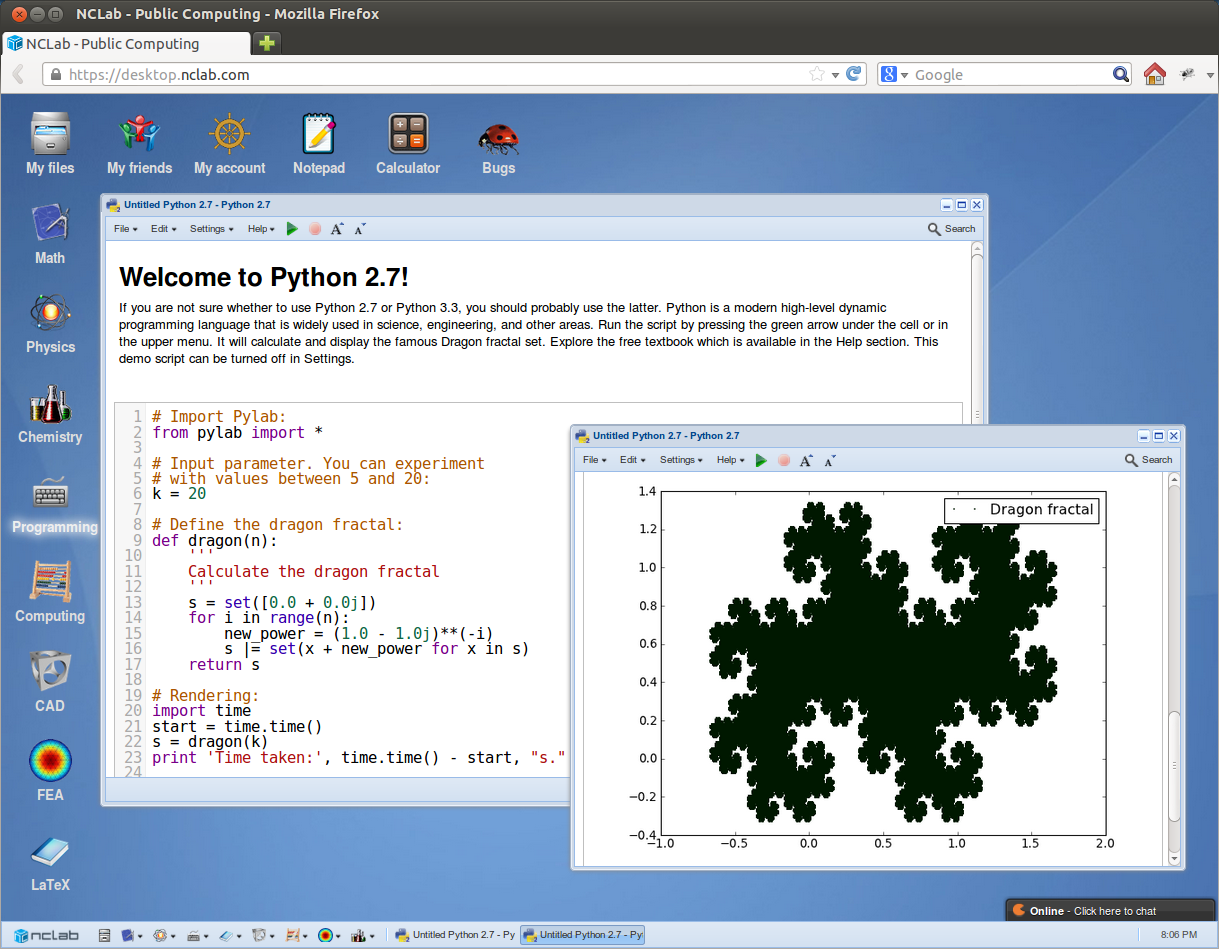
\includegraphics[width=0.9\textwidth]{img/python.png}
\end{center}
\vspace{-2mm}
\caption{Launching a new Python project.}
\label{fig:python}
\end{figure}


\subsection{Hello, World!}

Click into the code cell and type {\tt print "Hello, World!"}.
Then click on the green arrow under the cell, and the text 
"Hello, World!" will be displayed 
in a new yellow {\em output cell} as shown in Fig. \ref{fig:python-2}.
\newpage
\begin{figure}[!ht]
\begin{center}
\includegraphics[width=0.9\textwidth]{img/python-2.png}
\end{center}
\vspace{-2mm}
\caption{Response received from the cloud is shown in a yellow output cell.}
\label{fig:python-2}
\end{figure}
\noindent
The blue and red labels on the left-hand side of cells can be turned
off in Settings, allowing a bit more space for editing.

\subsection{Code, output, and descriptive cells}

There are three types of cells in the Python worksheet:
\begin{itemize}
\item {\em code cells} for entering computer code, 
\item {\em output cells} to display results, 
\item {\em descriptive cells} for textual and graphical descriptions.
\end{itemize} 
Code cells as well as descriptive cells can be added via buttons 
located under any code or descriptive cell. Each cell can be removed by clicking on the red 
remove button below the cell. All output cells can be removed at once via {\em Remove all output} 
option in the Edit menu. Pressing the green arrow button in the upper menu will run all code 
cells in the project. Clicking on the green arrow under a code cell will run only the contents 
of that particular code cell. 

%%%%%%%%%%%%%%%%%%%%%%%%%%%%%%%%%%%%%%%%%%%%%%%%%%%%%%%%%%%%%%%%%%%%%%

\section{Using Python as a Calculator} \label{sec:calc}

\subsection{Objectives}

\begin{itemize}
\item Learn how to use Python for elementary as well as advanced math operations.
\item Learn how to work with mathematical functions, fractions, random numbers 
      and complex numbers.
\end{itemize}
Python can be used as an advanced scientific calculator -- no need to own a TI-89 (\$150 value). 
As a matter of fact, NCLab is much more powerful -- a TI-89 hardly could compete with thousands 
of processors under NCLab's hood. 
In this textbook we will learn how to use this computing power. Let us begin with the simplest math 
operations. The rest of this section is fairly slow, so feel free to skip to Section 3
should it be too boring -- you can always return to it later.

\subsection{Addition and subtraction}

Launch a new Python project and in the code cell type:\\

\begin{bbox}
\begin{verbatim}
3 + 6
\end{verbatim}
\end{bbox}
\vspace{6mm}

\noindent
Then click on the green arrow under the cell. The output should be displayed quickly:\\

\begin{ybox}
\begin{verbatim}
9
\end{verbatim}
\end{ybox}
\vspace{6mm}

\noindent
Of course you can add real numbers too:\\

\begin{bbox}
\begin{verbatim}
3.2 + 6.31
\end{verbatim}
\end{bbox}
\vspace{6mm}

\noindent
Output:\\

\begin{ybox}
\begin{verbatim}
9.51
\end{verbatim}
\end{ybox}
\vspace{6mm}

\noindent
Two numbers can be subtracted using the minus sign:\\

\begin{bbox}
\begin{verbatim}
7.5 - 2.1
\end{verbatim}
\end{bbox}
\vspace{6mm}

\noindent
Output:\\

\begin{ybox}
\begin{verbatim}
5.4
\end{verbatim}
\end{ybox}
\vspace{6mm}

\noindent

\subsection{Multiplication}
Multiplication is done using the asterisk  '{\tt *}' symbol as in\\

\begin{bbox}
\begin{verbatim}
3 * 12
\end{verbatim}
\end{bbox}
\vspace{6mm}

\noindent
Output:\\

\begin{ybox}
\begin{verbatim}
36
\end{verbatim}
\end{ybox}
\vspace{6mm}

\noindent
Indeed, real numbers can be multiplied as well:\\

\begin{bbox}
\begin{verbatim}
3.7 * 12.17
\end{verbatim}
\end{bbox}
\vspace{6mm}

\noindent
Output:\\

\begin{ybox}
\begin{verbatim}
45.029
\end{verbatim}
\end{ybox}
\vspace{6mm}

\noindent

\subsection{Division}
The forward slash '{\tt /}' symbol is used for division:\\

\begin{bbox}
\begin{verbatim}
30 / 5
\end{verbatim}
\end{bbox}
\vspace{6mm}

\noindent
Output:\\

\begin{ybox}
\begin{verbatim}
6
\end{verbatim}
\end{ybox}
\vspace{6mm}

\noindent
However, we need to be careful. Look at this:\\

\begin{bbox}
\begin{verbatim}
33 / 5
\end{verbatim}
\end{bbox}
\vspace{6mm}

\noindent
Output:\\

\begin{ybox}
\begin{verbatim}
6
\end{verbatim}
\end{ybox}
\vspace{6mm}

\noindent
This is not correct! But why? The answer is that since the numbers {\tt 33} and {\tt 5}
are both integers, the result is automatically converted to an integer. This is how it works 
in all major computer languages including C, C++, Fortran, Python and others. The
correct way of using division is to represent at least one of the numbers as a real number.
Adding a decimal point is enough for that. Then the result is automatically converted 
to a real number:\\

\begin{bbox}
\begin{verbatim}
33. / 5
\end{verbatim}
\end{bbox}
\vspace{6mm}

\noindent
yields\\

\begin{ybox}
\begin{verbatim}
6.6
\end{verbatim}
\end{ybox}
\vspace{6mm}

\noindent
An alternative way of turning an integer into a real number, which 
also works for variables, is using the function {\tt float()}. Then
the above division could be done as follows:\\

\begin{bbox}
\begin{verbatim}
float(33) / 5
\end{verbatim}
\end{bbox}
\vspace{6mm}

\noindent
Output:\\

\begin{ybox}
\begin{verbatim}
6.6
\end{verbatim}
\end{ybox}
\vspace{6mm}

\noindent
Once we understand the behavior, we can use it to our advantage. For example,
we can calculate how many times a dozen fits into a thousand:\\

\begin{bbox}
\begin{verbatim}
1000 / 12
\end{verbatim}
\end{bbox}
\vspace{6mm}

\noindent
Output:\\

\begin{ybox}
\begin{verbatim}
83
\end{verbatim}
\end{ybox}
\vspace{6mm}

\noindent
By calculating {\tt 1000 - 83 * 12} we obtain {\tt 4} which is the remainder of the 
integer division. In fact the remainder can be calculated in a simpler way
using the modulo operator that will be introduced in the next paragraph.\\

\noindent
In summary:\\

\begin{gbox}
\begin{center}
Keep in mind that division is a tricky operation. Failure to convert at least one operand 
to a real number can be a source of mistakes that are very hard to find.
\end{center}
\end{gbox}

\subsection{Modulo}
The last of the common arithmetic operations is {\em modulo} (remainder 
after integer division). In Python modulo is represented via the percent symbol '{\tt \%}':\\

\begin{bbox}
\begin{verbatim}
6 % 4
\end{verbatim}
\end{bbox}
\vspace{6mm}

\noindent
Output:\\

\begin{ybox}
\begin{verbatim}
2
\end{verbatim}
\end{ybox}
\vspace{6mm}

\noindent
Modulo can be applied to real numbers as well:\\

\begin{bbox}
\begin{verbatim}
12.5 % 2.0 
\end{verbatim}
\end{bbox}
\vspace{6mm}

\noindent
Output:\\

\begin{ybox}
\begin{verbatim}
0.5
\end{verbatim}
\end{ybox}
\vspace{6mm}

\noindent

\subsection{Powers}
For exponents, such as in $2^4$, Python has a double-star
symbol \ '{\tt **}':\\

\begin{bbox}
\begin{verbatim}
2**4
\end{verbatim}
\end{bbox}
\vspace{6mm}

\noindent
Output:\\

\begin{ybox}
\begin{verbatim}
16
\end{verbatim}
\end{ybox}
\vspace{6mm}

\noindent
Both the base and the exponent can be real numbers:\\

\begin{bbox}
\begin{verbatim}
3.2**2.5
\end{verbatim}
\end{bbox}
\vspace{6mm}

\noindent
Output:\\

\begin{ybox}
\begin{verbatim}
18.31786887167828
\end{verbatim}
\end{ybox}
\vspace{6mm}

\noindent
But we have to be careful with negative numbers:\\

\begin{bbox}
\begin{verbatim}
(-3.2)**2.5
\end{verbatim}
\end{bbox}
\vspace{6mm}

\noindent
Output:\\

\begin{ybox}
\begin{Verbatim}[commandchars=\\\{\}]
\PY{n}{Traceback} \PY{p}{(}\PY{n}{most} \PY{n}{recent} \PY{n}{call} \PY{n}{last}\PY{p}{)}\PY{p}{:}
  \PY{n}{File} \PY{l+s}{"}\PY{l+s}{<nclab>}\PY{l+s}{"}\PY{p}{,} \PY{n}{line} \PY{l+m+mi}{1}\PY{p}{,} \PY{n}{in} \PY{o}{<}\PY{n}{module}\PY{o}{>}
\PY{n+ne}{ValueError}\PY{p}{:} \PY{n}{negative} \PY{n}{number} \PY{n}{cannot} \PY{n}{be} \PY{n}{raised} \PY{n}{to} \PY{n}{a} \PY{n}{fractional} 
\PY{n}{power}
\end{Verbatim}
\end{ybox}
\vspace{6mm}

\subsection{Priority of operators}
Python respects the standard priority of operators that 
is standard in mathematics:

\begin{itemize} 
\item Round brackets '{\tt (...)}'have the highest priority,
\item then exponentiation '{\tt **}', 
\item then multiplication '{\tt *}', division '{\tt /}' and modulo '{\tt \%}', 
\item the lowest priority have addition '{\tt +}' and subtraction '{\tt -}',
\item operations with the same priority are evaluated from left to right -- for
      example the result of {\tt 20 / 10 * 2} is {\tt 4}. 
\end{itemize}
Note that no other brackets such as {\tt \{ \}} and {\tt [ ]} are 
admissible in mathematical expressions. The reason is that they have a different 
function in the programming language.
To illustrate the priority of operations, we evaluate the following 
expression:\\

\begin{bbox}
\begin{verbatim}
3**4 / 27 * 5 + 3 * 5
\end{verbatim}
\end{bbox}
\vspace{6mm}

\noindent
Output:\\

\begin{ybox}
\begin{verbatim}
30
\end{verbatim}
\end{ybox}
\vspace{6mm}

\noindent
If we are not sure, it never hurts to use round brackets:\\

\begin{bbox}
\begin{verbatim}
(3**4) / 27 * 5 + 3 * 5
\end{verbatim}
\end{bbox}
\vspace{6mm}

\noindent
Output:\\

\begin{ybox}
\begin{verbatim}
30
\end{verbatim}
\end{ybox}
\vspace{6mm}



\subsection{Using empty characters makes your code more readable}
Your code will be much more readable if you use empty
characters on either side of arithmetic symbols, as well as 
after commas. Hence, you should never write things like \\

\begin{bbox}
\begin{verbatim}
sin(x+y)+f(x,y,z)*5-2.4.
\end{verbatim}
\end{bbox}
\vspace{6mm}

\noindent
Instead, the same can be written in a much more reader-friendly form as\\

\begin{bbox}
\begin{verbatim}
sin(x + y) + f(x, y, z) * 5 - 2.4.
\end{verbatim}
\end{bbox}
\vspace{6mm}

\noindent

\subsection{Using mathematical functions}

In order to calculate square roots, exponentials, sines, cosines, tangents, and many other 
math functions, the best way is to import Numpy. Numpy is a powerful Python library 
for numerical computations. To import it, just include the following 
line in your code:\\

\begin{bbox}
\begin{verbatim}
from numpy import *
\end{verbatim}
\end{bbox}
\vspace{6mm}

\noindent
Here the symbol '{\tt *}' stands for "everything". If you wanted to import just one or two 
functions, you could do that as well by just giving their names, separated by commas. 
After Numpy is imported, we can calculate, for example, $e^2$:\\

\begin{bbox}
\begin{verbatim}
exp(2)
\end{verbatim}
\end{bbox}
\vspace{6mm}

\noindent
Output:\\

\begin{ybox}
\begin{verbatim}
7.3890560989306504
\end{verbatim}
\end{ybox}
\vspace{6mm}

\noindent
Elementary functions (and constants) that one can import from Numpy are listed
below. We also show their arguments for clarity, but the functions are imported without 
them. For example, the absolute value function is imported via {\tt from numpy import abs}.\\

%{\small
\begin{center}
\begin{tabular}{|l|l|}
\hline
\ pi &  \ $\pi$\\
\ abs($x$) &\   absolute value of $x$\\
\ arccos($x$) &\   inverse cosine of $x$ \\
\ arccosh($x$) &\   inverse hyperbolic cosine of $x$ \\
\ arcsin($x$) &\  inverse sine of $x$ \\
\ arcsinh($x$) &\  inverse hyperbolic sine of $x$ \\
\ arctan($x$) &\  inverse tangent of $x$ \\
\ arctanh($x$) &\  inverse hyperbolic tangent of $x$ \\
\ arctan2($x_1$, $x_2$) \ \ \ &\  arc tangent of $x_1/x_2$ choosing the quadrant correctly \\
\ cos($x$) &\  cosine of $x$ \\
\ cosh($x$) &\  hyperbolic tangent of $x$ \\
\ exp($x$) &\  $e^x$ \\
\ log($x$) &\  natural logarithm of $x$ \\
\ pow($a$, $b$) &\  $a^b$ (same as "a**b")\\
\ sin($x$) &\  sine of $x$ \\
\ sinh($x$) &\  hyperbolic sine of $x$ \\
\ sqrt($x$) &\  square root of $x$ \\
\ tan($x$) &\  tangent of $x$\\
\ tanh($x$) &\  hyperbolic tangent of $x$ \\
\hline
\end{tabular}
\end{center}
%}
\vspace{4mm}
\noindent

\noindent
In summary:\\

\begin{gbox}
\begin{center}
Python provides many readily available mathematical functions via the Numpy library.
To use them, import them via the command {\tt from numpy import *}
\end{center}
\end{gbox}


\subsection{\ \ Fractions}

Python makes operation with fractions easy via the {\tt Fraction}
function that is imported from the {\tt fractions} library:\\

\begin{bbox}
\begin{verbatim}
from fractions import Fraction
\end{verbatim}
\end{bbox}
\vspace{6mm}

\noindent
A fraction such as 4/7 can be defined simply as {\tt Fraction(4, 7)}. 
Fractions can be used with the same operations as numbers, and the result 
of such an operation is a {\tt Fraction}. For example\\

\begin{bbox}
\begin{verbatim}
Fraction(2, 6) + Fraction(2, 3)
\end{verbatim}
\end{bbox}
\vspace{6mm}

\noindent
yields\\

\begin{ybox}
\begin{verbatim}
Fraction(1, 1)
\end{verbatim}
\end{ybox}
\vspace{6mm}

\noindent
Another example: \\

\begin{bbox}
\begin{verbatim}
Fraction(2, 6) / Fraction(2, 3)
\end{verbatim}
\end{bbox}
\vspace{6mm}

\noindent
results into\\

\begin{ybox}
\begin{verbatim}
Fraction(1, 2)
\end{verbatim}
\end{ybox}
\vspace{6mm}

\noindent
The {\tt fractions} library also provides the useful function {\tt gcd()} that 
calculates the Greatest Common Divisor (GCD) of two integers. It is imported via \\

\begin{bbox}
\begin{verbatim}
from fractions import gcd
\end{verbatim}
\end{bbox}
\vspace{6mm}

\noindent
For illustration let us calculate the GCD of 867 and 629:\\

\begin{bbox}
\begin{verbatim}
gcd(867, 629)
\end{verbatim}
\end{bbox}
\vspace{6mm}

\noindent
The output is \\

\begin{ybox}
\begin{verbatim}
17
\end{verbatim}
\end{ybox}
\vspace{6mm}

\noindent

\subsection{\ \ Random numbers}

Python provides a random number generator via the {\tt random()} function that 
can be imported from the {\tt random} library:\\

\begin{bbox}
\begin{verbatim}
from random import random
\end{verbatim}
\end{bbox}
\vspace{6mm}

\noindent
This function returns a random real number between 0 and 1. For 
example,\\

\begin{bbox}
\begin{verbatim}
random()
\end{verbatim}
\end{bbox}
\vspace{6mm}

\noindent
yields\\

\begin{ybox}
\begin{verbatim}
0.871979925682207
\end{verbatim}
\end{ybox}
\vspace{6mm}

\noindent
Sometimes we need to generate random integers rather than real numbers.
This is easy. For illustration, a random integer {\tt n} between 1 and 3 can be 
generated via the code\\

\begin{bbox}
\begin{verbatim}
a = random()
n = int(3*a + 1)
\end{verbatim}
\end{bbox}
\vspace{6mm}

\noindent
Here the function {\tt int()} will erase the decimal part of the real number, converting 
it to an integer.


\subsection{\ \ Complex numbers}

Complex numbers are always represented as two floating point numbers, the 
real and imaginary part. Appending '{\tt j}' or  '{\tt J}' to a real number
makes it imaginary:\\

\begin{bbox}
\begin{verbatim}
1j * 1J
\end{verbatim}
\end{bbox}
\vspace{6mm}

\noindent
Output:\\

\begin{ybox}
\begin{verbatim}
(-1+0j)
\end{verbatim}
\end{ybox}
\vspace{6mm}

\noindent
This is one way to define complex numbers:\\

\begin{bbox}
\begin{verbatim}
1 + 3j
\end{verbatim}
\end{bbox}
\vspace{6mm}

\noindent
Output:\\

\begin{ybox}
\begin{verbatim}
(1+3j)
\end{verbatim}
\end{ybox}
\vspace{6mm}

\noindent
Another way is to use the command {\tt complex}:\\

\begin{bbox}
\begin{verbatim}
complex(1, 3)
\end{verbatim}
\end{bbox}
\vspace{6mm}

\noindent
Output:\\

\begin{ybox}
\begin{verbatim}
(1+3j)
\end{verbatim}
\end{ybox}
\vspace{6mm}

\noindent
All arithmetic operations that are used for real numbers can be 
used for complex numbers as well, for example:\\

\begin{bbox}
\begin{verbatim}
(1 + 2j) / (1 + 1j)
\end{verbatim}
\end{bbox}
\vspace{6mm}

\noindent
Output:\\

\begin{ybox}
\begin{verbatim}
(1.5+0.5j)
\end{verbatim}
\end{ybox}
\vspace{6mm}

\noindent
To extract the real and imaginary parts of a complex number {\tt z}, use {\tt z.real}
and {\tt z.imag}. Use {\tt abs()} to get the absolute value:\\

\begin{bbox}
\begin{verbatim}
a = 3 + 4j
a.real
a.imag
abs(a)
\end{verbatim}
\end{bbox}
\vspace{6mm}

\noindent
Output:\\

\begin{ybox}
\begin{verbatim}
3
4
5
\end{verbatim}
\end{ybox}
\vspace{6mm}

\noindent

%%%%%%%%%%%%%%%%%%%%%%%%%%%%%%%%%%%%%%%%%%%%%%%%%%%%%%%%%%%%%%%%%%%%%%%%%%%

\section{Functions}

\subsection{Objectives}

\begin{itemize}
\item Review what we know about functions from Karel the Robot.
\item Learn that in Python, functions can accept input arguments.
\item Learn to use default arguments and return multiple values.
\end{itemize}

\subsection{Defining new functions}

The purpose of creating custom functions is to make selected functionality 
easily reusable. In this way we can avoid code duplication, and bring more 
structure and transparency into our programs. \\

\noindent
In Karel the Robot, custom functions were similar to commands but 
additionally, they could return values. For example, a function 
{\tt turnsouth}, that turns the robot to face South and makes him 
return his GPS coordinates, looks as follows:\\

\begin{bbox}
\begin{verbatim}
def turnsouth
    while not north 
        left
    repeat 2
        left
    return [gpsx, gpsy]
\end{verbatim}
\end{bbox}
\vspace{6mm}

\noindent
In Python, the definition of a new function also begins with the keyword {\tt def},
but we moreover have to use round brackets for input arguments and the colon '{\tt :}'
at the end of the line. For example, the following function adds two numbers
and returns the result:\\

\begin{bbox}
\begin{Verbatim}[commandchars=\\\{\}]
\PY{k}{def} \PY{n+nf}{add}\PY{p}{(}\PY{n}{a}\PY{p}{,} \PY{n}{b}\PY{p}{)}\PY{p}{:}
    \PY{k}{return} \PY{n}{a} \PY{o}{+} \PY{n}{b}
\end{Verbatim}
\end{bbox}
\vspace{6mm}

\noindent
The round brackets in the function definition are mandatory even if no arguments are passed
but  the {\tt return} statement can be omitted if not needed.
The two lines of code above 
are a {\em function declaration} only -- the function is not called. 
In order to call the function, we need to write one additional line:\\

\begin{bbox}
\begin{Verbatim}[commandchars=\\\{\}]
\PY{k}{print} \PY{l+s}{"}\PY{l+s}{5 + 3 is}\PY{l+s}{"}\PY{p}{,} \PY{n}{add}\PY{p}{(}\PY{l+m+mi}{5}\PY{p}{,} \PY{l+m+mi}{3}\PY{p}{)}
\end{Verbatim}
\end{bbox}
\vspace{6mm}

\noindent
This will produce the following output:\\

\begin{ybox}
\begin{Verbatim}[commandchars=\\\{\}]
\PY{l+m+mi}{5} \PY{o}{+} \PY{l+m+mi}{3} \PY{l+m+mi}{is} \PY{l+m+mi}{8}
\end{Verbatim}
\end{ybox}
\vspace{6mm}

\noindent
In most cases, functions are defined to process some input arguments 
and to return some output values. However, this does not apply always.
The following function does not take any arguments 
and it does not return anything:\\

\begin{bbox}
\begin{Verbatim}[commandchars=\\\{\}]
\PY{k}{def} \PY{n+nf}{print_hello}\PY{p}{(}\PY{p}{)}\PY{p}{:}
    \PY{k}{print} \PY{l+s}{"}\PY{l+s}{Hello!}\PY{l+s}{"}
\end{Verbatim}
\end{bbox}
\vspace{6mm}

\noindent

\subsection{Passing arbitrary arguments}

Python does not require that we specify the type of function arguments. 
What does it mean? The above function {\tt add(a, b)} works for real
numbers, complex numbers, vectors, strings, and any other 
objects where the operation '+' is defined. Let's try this:\\

\begin{bbox}
\begin{Verbatim}[commandchars=\\\{\}]
\PY{k}{def} \PY{n+nf}{add}\PY{p}{(}\PY{n}{a}\PY{p}{,} \PY{n}{b}\PY{p}{)}\PY{p}{:}
    \PY{k}{return} \PY{n}{a} \PY{o}{+} \PY{n}{b}

\PY{n}{word1} \PY{o}{=} \PY{l+s}{"}\PY{l+s}{Good }\PY{l+s}{"}
\PY{n}{word2} \PY{o}{=} \PY{l+s}{"}\PY{l+s}{Evening!}\PY{l+s}{"}
\PY{k}{print} \PY{n}{add}\PY{p}{(}\PY{n}{word1}\PY{p}{,} \PY{n}{word2}\PY{p}{)}
\end{Verbatim}
\end{bbox}
\vspace{6mm}

\noindent
Output:\\

\begin{ybox}
\begin{Verbatim}[commandchars=\\\{\}]
\PY{n}{Good} \PY{n}{Evening!}
\end{Verbatim}
\end{ybox}
\vspace{6mm}

\noindent
This makes Python very intuitive and easy to use compared to other languages. 
For example, to do the same as above, in C/C++ we would have to introduce different functions 
for real numbers, for complex numbers, for strings, and any other data 
types. They would look as follows:\\

\begin{bbox}
\begin{verbatim}
double add(double a, double b)
{
  return a + b;
}
\end{verbatim}
\end{bbox}
\vspace{6mm}

\noindent
and\\

\begin{bbox}
\begin{verbatim}
# include <complex.h>
complex add(complex a, complex b)
{
  return a + b;
}
\end{verbatim}
\end{bbox}
\vspace{6mm}

\noindent
and \\

\begin{bbox}
\begin{verbatim}
void add(const char* a_in, const char* b_in, char* c_out)
{
  strcpy(c_out, a_in);
  strcat(c_out, b_in);
  return;
}
\end{verbatim}
\end{bbox}
\vspace{6mm}

\noindent
etc. While C++ is a great language, technical details like this 
make it more difficult for beginners.

\subsection{Returning multiple values}

Python functions can return multiple values which often comes handy.
For example, the following function returns the 
second, third, and fourth powers of a number:\\

\begin{bbox}
\begin{Verbatim}[commandchars=\\\{\}]
\PY{k}{def} \PY{n+nf}{powers}\PY{p}{(}\PY{n}{a}\PY{p}{)}\PY{p}{:}
    \PY{k}{return} \PY{n}{a}\PY{o}{*}\PY{o}{*}\PY{l+m+mi}{2}\PY{p}{,} \PY{n}{a}\PY{o}{*}\PY{o}{*}\PY{l+m+mi}{3}\PY{p}{,} \PY{n}{a}\PY{o}{*}\PY{o}{*}\PY{l+m+mi}{4}
\end{Verbatim}
\end{bbox}
\vspace{6mm}

\noindent
This is how the function is used:\\

\begin{bbox}
\begin{Verbatim}[commandchars=\\\{\}]
\PY{n}{var1} \PY{o}{=} \PY{l+m+mi}{2}
\PY{k}{print} \PY{l+s}{"}\PY{l+s}{Powers are}\PY{l+s}{"}\PY{p}{,} \PY{n}{powers}\PY{p}{(}\PY{n}{var1}\PY{p}{)}
\end{Verbatim}
\end{bbox}
\vspace{6mm}

\noindent
Output:\\

\begin{ybox}
\begin{Verbatim}[commandchars=\\\{\}]
\PY{n}{Powers} \PY{n}{are} \PY{p}{(}\PY{l+m+mi}{4}\PY{p}{,} \PY{l+m+mi}{8}\PY{p}{,} \PY{l+m+mi}{16}\PY{p}{)}
\end{Verbatim}
\end{ybox}
\vspace{6mm}

\noindent
We can also store the returned values in three separate variables:\\

\begin{bbox}
\begin{Verbatim}[commandchars=\\\{\}]
\PY{n}{var1} \PY{o}{=} \PY{l+m+mi}{3}
\PY{n}{p2}\PY{p}{,} \PY{n}{p3}\PY{p}{,} \PY{n}{p4} \PY{o}{=} \PY{n}{powers}\PY{p}{(}\PY{n}{var1}\PY{p}{)}
\PY{k}{print} \PY{l+s}{"}\PY{l+s}{Powers are}\PY{l+s}{"}\PY{p}{,} \PY{n}{p2}\PY{p}{,} \PY{n}{p3}\PY{p}{,} \PY{n}{p4}
\end{Verbatim}
\end{bbox}
\vspace{6mm}

\noindent
Output:\\

\begin{ybox}
\begin{Verbatim}[commandchars=\\\{\}]
\PY{n}{Powers} \PY{n}{are} \PY{l+m+mi}{9} \PY{l+m+mi}{27} \PY{l+m+mi}{81}
\end{Verbatim}
\end{ybox}
\vspace{6mm}

\noindent
Again, for comparison let's see how this would be handled in C/C++. The asterisks
in the code below are {\em pointers}, an additional programming concept that 
one needs to learn and utilize here:\\

\begin{bbox}
\begin{verbatim}
void powers(double a, double* p2, double* p2, double* p3)
{
  *p2 = pow(a, 2);
  *p3 = pow(a, 3);
  *p4 = pow(a, 4);
  return;
}

int main()
{
  double p1, p2, p3;
  double a = 2;
  powers(a, &p2, &p2, &p3);
  printf("Powers are %g, %g, %g.\n", p2, p3, p4);
}
\end{verbatim}
\end{bbox}
\vspace{6mm}

\noindent

\subsection{Using default arguments}

Have you ever been to Holland? It is the most bicycle friendly place in the world. Imagine that you 
work for the Holland Census Bureau. Your job is to ask 10000 
people how they go to work, and enter their answers into a database. 
The program for entering data into the database was written by one of 
your colleagues, and it can be used as follows:\\

\begin{bbox}
\begin{Verbatim}[commandchars=\\\{\}]
\PY{n}{add\PYZus{}database\PYZus{}entry}\PY{p}{(}\PY{l+s}{"}\PY{l+s}{John}\PY{l+s}{"}\PY{p}{,} \PY{l+s}{"}\PY{l+s}{Smith}\PY{l+s}{"}\PY{p}{,} \PY{l+s}{"}\PY{l+s}{walks}\PY{l+s}{"}\PY{p}{)}
\end{Verbatim}
\end{bbox}
\vspace{6mm}

\noindent
or \\

\begin{bbox}
\begin{Verbatim}[commandchars=\\\{\}]
\PY{n}{add\PYZus{}database\PYZus{}entry}\PY{p}{(}\PY{l+s}{"}\PY{l+s}{Louis}\PY{l+s}{"}\PY{p}{,} \PY{l+s}{"}\PY{l+s}{Armstrong}\PY{l+s}{"}\PY{p}{,} \PY{l+s}{"}\PY{l+s}{bicycle}\PY{l+s}{"}\PY{p}{)}
\end{Verbatim}
\end{bbox}
\vspace{6mm}

\noindent
or\\

\begin{bbox}
\begin{Verbatim}[commandchars=\\\{\}]
\PY{n}{add\PYZus{}database\PYZus{}entry}\PY{p}{(}\PY{l+s}{"}\PY{l+s}{Jim}\PY{l+s}{"}\PY{p}{,} \PY{l+s}{"}\PY{l+s}{Bridger}\PY{l+s}{"}\PY{p}{,} \PY{l+s}{"}\PY{l+s}{horse}\PY{l+s}{"}\PY{p}{)}
\end{Verbatim}
\end{bbox}
\vspace{6mm}

\noindent
etc. Since you are in Holland, it can be expected that $99 \%$ of people 
are using the bicycle. In principle you could call the function {\tt add\_database\_entry()} 
to enter each answer, but with 9900 bicyclists out of 10000 respondents you would have to 
type the word {\tt "bicycle"} MANY times. 

Fortunately, Python offers a smarter way to do this. We can define a new function \\

\begin{bbox}
\begin{Verbatim}[commandchars=\\\{\}]
\PY{k}{def} \PY{n+nf}{enter}\PY{p}{(}\PY{n}{first}\PY{p}{,} \PY{n}{last}\PY{p}{,} \PY{n}{transport} \PY{o}{=} \PY{l+s}{"}\PY{l+s}{bicycle}\PY{l+s}{"}\PY{p}{)}\PY{p}{:}
    \PY{n}{enter\PYZus{}into\PYZus{}database}\PY{p}{(}\PY{n}{first}\PY{p}{,} \PY{n}{last}\PY{p}{,} \PY{n}{transport}\PY{p}{)}
\end{Verbatim}
\end{bbox}
\vspace{6mm}

\noindent
This is a simple ({"thin"}) {\em wrapper} to the function {\tt add\_database\_entry()} 
that allows us to omit the third argument in the function call and autocomplete 
it with a {\em default argument} {\tt "bicycle"}. In other words, now we do not have to 
type {\tt "bicycle"} for Louis Armstrong or any other bicyclist:\\

\begin{bbox}
\begin{Verbatim}[commandchars=\\\{\}]
\PY{n}{enter}\PY{p}{(}\PY{l+s}{"}\PY{l+s}{Louis}\PY{l+s}{"}\PY{p}{,} \PY{l+s}{"}\PY{l+s}{Armstrong}\PY{l+s}{"}\PY{p}{)}
\end{Verbatim}
\end{bbox}
\vspace{6mm}

\noindent
Only if we meet a rare someone who uses a car, we type \\

\begin{bbox}
\begin{Verbatim}[commandchars=\\\{\}]
\PY{n}{enter}\PY{p}{(}\PY{l+s}{"}\PY{l+s}{Niki}\PY{l+s}{"}\PY{p}{,} \PY{l+s}{"}\PY{l+s}{Lauda}\PY{l+s}{"}\PY{p}{,} \PY{l+s}{"}\PY{l+s}{car}\PY{l+s}{"}\PY{p}{)}
\end{Verbatim}
\end{bbox}
\vspace{6mm}

\noindent
Another example: Let us return to the function {\tt add()}, and let us 
imagine that very often (but not always) the second number that we
are adding is 10. Then it makes sense to write the function {\tt add()}
as follows:\\

\begin{bbox}
\begin{Verbatim}[commandchars=\\\{\}]
\PY{k}{def} \PY{n+nf}{add}\PY{p}{(}\PY{n}{a}\PY{p}{,} \PY{n}{b} \PY{o}{=} \PY{l+m+mi}{10}\PY{p}{)}\PY{p}{:}
    \PY{k}{return} \PY{n}{a} \PY{o}{+} \PY{n}{b}
\end{Verbatim}
\end{bbox}
\vspace{6mm}

\noindent
The function will work as before when called with two arguments: \\

\begin{bbox}
\begin{Verbatim}[commandchars=\\\{\}]
\PY{n}{A} \PY{o}{=} \PY{l+m+mi}{5}
\PY{n}{B} \PY{o}{=} \PY{l+m+mi}{1}
\PY{n}{add}\PY{p}{(}\PY{n}{A}\PY{p}{,} \PY{n}{B}\PY{p}{)}
\end{Verbatim}
\end{bbox}
\vspace{6mm}

\noindent
Output:\\

\begin{ybox}
\begin{Verbatim}[commandchars=\\\{\}]
\PY{l+m+mi}{6}
\end{Verbatim}
\end{ybox}
\vspace{6mm}

\noindent
But it can also be called with the second argument omitted:\\

\begin{bbox}
\begin{Verbatim}[commandchars=\\\{\}]
\PY{n}{A} \PY{o}{=} \PY{l+m+mi}{5}
\PY{n}{add}\PY{p}{(}\PY{n}{A}\PY{p}{)}
\end{Verbatim}
\end{bbox}
\vspace{6mm}

\noindent
Output:\\

\begin{ybox}
\begin{Verbatim}[commandchars=\\\{\}]
\PY{l+m+mi}{15}
\end{Verbatim}
\end{ybox}

\subsection*{Few rules to remember}


(1) Default arguments need to be introduced {\bf after} standard (non-default) arguments. In other words, the 
      following code will result into an error:\\

\begin{bbox}
\begin{Verbatim}[commandchars=\\\{\}]
\PY{k}{def} \PY{n+nf}{add}\PY{p}{(}\PY{n}{a} \PY{o}{=} \PY{l+m+mi}{5}\PY{p}{,} \PY{n}{b}\PY{p}{)}\PY{p}{:}
    \PY{k}{return} \PY{n}{a} \PY{o}{+} \PY{n}{b}
\end{Verbatim}
\end{bbox}
\vspace{6mm}

\noindent
This is the error message:\\

\begin{ybox}
\begin{Verbatim}[commandchars=\\\{\}]
\PY{n}{File} \PY{l+s}{"}\PY{l+s}{<nclab>}\PY{l+s}{"}\PY{p}{,} \PY{n}{line} \PY{l+m+mi}{1}
\PY{n+ne}{SyntaxError}\PY{p}{:} \PY{n}{non}\PY{o}{-}\PY{n}{default} \PY{n}{argument} \PY{n}{follows} \PY{n}{default} \PY{n}{argument}\PY{o}{.}
\end{Verbatim}
\end{ybox}
\vspace{6mm}

\noindent
(2) If multiple default arguments are present, they have to follow the non-default ones.
      If the number of arguments in the function call is less than the total number of default and non-default
      arguments, then first all non-default arguments are assigned, and then the default ones from 
      left to right. To illustrate this, assume the function:\\

\begin{bbox}
\begin{Verbatim}[commandchars=\\\{\}]
\PY{k}{def} \PY{n+nf}{add}\PY{p}{(}\PY{n}{x}\PY{p}{,} \PY{n}{a} \PY{o}{=} \PY{l+m+mi}{2}\PY{p}{,} \PY{n}{b} \PY{o}{=} \PY{l+m+mi}{3}\PY{p}{)}\PY{p}{:}
    \PY{k}{return} \PY{n}{x} \PY{o}{+} \PY{n}{a} \PY{o}{+} \PY{n}{b}
\end{Verbatim}
\end{bbox}
\vspace{6mm}

\noindent
This function can be called as follows:\\

\begin{bbox}
\begin{Verbatim}[commandchars=\\\{\}]
\PY{k}{print} \PY{n}{add}\PY{p}{(}\PY{l+m+mi}{1}\PY{p}{)}
\end{Verbatim}
\end{bbox}
\vspace{6mm}

\noindent
In this case, the value {\tt 1} is assigned to {\tt x} and {\tt a} and {\tt b} take the default values.
The output is \\

\begin{ybox}
\begin{Verbatim}[commandchars=\\\{\}]
\PY{l+m+mi}{6}
\end{Verbatim}
\end{ybox}
\vspace{6mm}

\noindent
When the function is called with just two values,\\

\begin{bbox}
\begin{Verbatim}[commandchars=\\\{\}]
\PY{k}{print} \PY{n}{add}\PY{p}{(}\PY{l+m+mi}{5}\PY{p}{,} \PY{l+m+mi}{6}\PY{p}{)}
\end{Verbatim}
\end{bbox}
\vspace{6mm}

\noindent
then the value {\tt 5} is assigned to {\tt x}, {\tt 6} to {\tt a}, and {\tt b} takes the default value {\tt 3}.
The output is\\

\begin{ybox}
\begin{Verbatim}[commandchars=\\\{\}]
\PY{l+m+mi}{14}
\end{Verbatim}
\end{ybox}
\vspace{6mm}

\noindent
However, it is always a good idea to be as transparent as possible. Therefore a better code is \\

\begin{bbox}
\begin{Verbatim}[commandchars=\\\{\}]
\PY{k}{print} \PY{n}{add}\PY{p}{(}\PY{l+m+mi}{1}\PY{p}{,} \PY{n}{a} \PY{o}{=} \PY{l+m+mi}{6}\PY{p}{)}
\end{Verbatim}
\end{bbox}
\vspace{6mm}

\noindent
The result is the same, {\tt 14}, but it is clear even to non-experts what is going on. Moreover,
in this way we can also define the value of {\tt b} without having to define the value of {\tt a}:\\

\begin{bbox}
\begin{Verbatim}[commandchars=\\\{\}]
\PY{k}{print} \PY{n}{add}\PY{p}{(}\PY{l+m+mi}{1}\PY{p}{,} \PY{n}{b} \PY{o}{=} \PY{l+m+mi}{6}\PY{p}{)}
\end{Verbatim}
\end{bbox}
\vspace{6mm}

\noindent
Now {\tt x} is {\tt 1}, {\tt a} has the default value {\tt 2} and the result is {\tt 9}.

%%%%%%%%%%%%%%%%%%%%%%%%%%%%%%%%%%%%%%%%%%%%%%%%%%%%%%%%%%%%%%%%%%%%%%

\section{Colors and Plotting} \label{sec:plotting}

\subsection{Objectives}

\begin{itemize}
\item Understand how colors are composed of Red, Green and Blue components.
\item Learn how to plot polygons, graphs of functions of one and two variables.
\item Learn how to plot 2D and 3D curves and surfaces.
\item Learn how to plot pie charts and bar charts.
\end{itemize}


\subsection{RGB colors}

According to the {\em additive color model} which is based on the human perception of colors,
every color can be obtained by mixing the shades of Red, Green and Blue. These are 
called {\em additive primary colors} or just {\em primary colors}. The resulting color depends on the proportions of the 
primary colors in the mix. It is customary to define these proportions by a number 
between 0 and 1 for each primary color. So, the resulting color is a triplet of 
real numbers between 0 and 1. For the primary colors we have\\

\begin{center}
\begin{tabular}{|c||c|c|c|}
\hline
\ Color & \ R \ & \ G \ & \ B \ \\
\hline
\hline
Red & 1 & 0 & 0\\
\hline
Green & 0 & 1 & 0\\
\hline
Blue & 0 & 0 & 1\\
\hline
\end{tabular}
\end{center}
\vspace{4mm}
These colors are shown in the following Fig. \ref{fig:rgb}.

\begin{figure}[!ht]
\begin{center}
\includegraphics[width=0.7\textwidth]{img/rgb.png}
\end{center}
\vspace{-2mm}
\caption{Left: pure red color [1, 0, 0]. Middle: pure green color [0, 1, 0]. Right; pure blue color [0, 0, 1].}
\label{fig:rgb}
\end{figure}
\noindent
When the proportions of all three primary colors are the same, the result is a shade of grey.
With [0, 0, 0] one obtains black, with [1, 1, 1] white. This is illustrated in Fig. \ref{fig:rgb2}.

\begin{figure}[!ht]
\begin{center}
\includegraphics[width=0.7\textwidth]{img/rgb2.png}
\end{center}
\vspace{-2mm}
\caption{Left: black color [0, 0, 0]. Middle: dark grey color [0.5, 0.5, 0.5]. Right; light grey color [0.9, 0.9, 0.9].}
%\vspace{-1cm}
\label{fig:rgb2}
\end{figure}
\noindent
\noindent
Guessing RGB codes is not easy. If you need to find the numbers representing your favorite color, 
the best way is to Google for "rgb color palette". You will find many pages that translate
colors into RGB codes. Most of them will have the colors represented by integer numbers 
between 0 and 255 (as opposed to the 0 to 1 scale). This is because these integers are easier 
to represent using bits and Bytes. However, it is sufficient to divide all three numbers by 255
to translate the color into the original unit scale. Fig. \ref{fig:rgb3} shows three "easy" colors
cyan, pink and yellow along with their RGB codes.

\begin{figure}[!ht]
\begin{center}
\includegraphics[width=0.7\textwidth]{img/rgb3.png}
\end{center}
\vspace{-2mm}
\caption{Left: cyan color [0, 1, 1]. Middle: pink color [1, 0, 1]. Right; yellow color [1, 1, 0].}
\label{fig:rgb3}
\end{figure}



\subsection{Plotting polylines and polygons}

In Python, plotting is done via the Pylab library. The Pylab {\tt plot()} function takes 
two arrays: $x$-coordinates and $y$-coordinates of points in the $xy$ plane. Between the 
points, the curve is interpolated linearly. Let us illustrate this on a simple 
example with just five points [0, 0], [1, 2], [2, 0.5], [3, 2.5] and [4, 0]:\\

\begin{bbox}
\begin{Verbatim}[commandchars=\\\{\}]
\PY{k+kn}{from} \PY{n+nn}{pylab} \PY{k+kn}{import} \PY{o}{*}
\PY{n}{x} \PY{o}{=} \PY{p}{[}\PY{l+m+mi}{0}\PY{p}{.}\PY{l+m+mi}{0}\PY{p}{,} \PY{l+m+mf}{1.0}\PY{p}{,} \PY{l+m+mf}{2.0}\PY{p}{,} \PY{l+m+mf}{3.0}\PY{p}{,} \PY{l+m+mf}{4.0}\PY{p}{]}
\PY{n}{y} \PY{o}{=} \PY{p}{[}\PY{l+m+mf}{0.0}\PY{p}{,} \PY{l+m+mf}{2.0}\PY{p}{,} \PY{l+m+mf}{0.5}\PY{p}{,} \PY{l+m+mf}{2.5}\PY{p}{,} \PY{l+m+mi}{0.0}\PY{p}{]}
\PY{n}{clf}\PY{p}{(}\PY{p}{)}
\PY{n}{plot}\PY{p}{(}\PY{n}{x}\PY{p}{,} \PY{n}{y}\PY{p}{)}
\PY{n}{lab}\PY{o}{.}\PY{n}{show}\PY{p}{(}\PY{p}{)}
\end{Verbatim}
\end{bbox}
\vspace{6mm}

\noindent
The commands {\tt clf()}, {\tt plot()} and {\tt lab.show()} do clear the canvas, 
plot the graph, and fetch the image from server, respectively.
The output is shown in Fig. \ref{fig:plot}.
\newpage

\begin{figure}[!ht]
\begin{center}
\hbox{}
\hspace{-6mm}
\includegraphics[width=0.56\textwidth]{img/plot.png}
\end{center}
\vspace{-2mm}
\caption{Polyline with five points.}
\label{fig:plot}
%\vspace{-1cm}
\end{figure}
\noindent
If the first and last points were the same,
then the polyline would form a closed loop and one would obtain a polygon.
The above plot was done using a default blue color. The color can be 
set by passing an optional parameter {\tt color = [R, G, B]} into the {\tt plot()}
function. For illustration, changing the fifth line in the last script to {\tt plot(x, y, color = [1, 0, 1])},
we obtain a pink polyline shown in Fig. \ref{fig:pinkplot}.

\begin{figure}[!ht]
\begin{center}
\hbox{}
\hspace{-6mm}
\includegraphics[width=0.56\textwidth]{img/pinkplot.png}
\end{center}
\vspace{-2mm}
\caption{Setting custom color.}
\label{fig:pinkplot}
\vspace{-1cm}
\end{figure}
\newpage


\subsection{Plotting functions of one variable}\label{plotting}


In the following we will discuss more options and show some useful techniques.
Let's say, for example, that we want to plot the function $f(x) = \sin(x)$
in the interval $(0, 2\pi)$. The array of $x$-coordinates of equidistant points 
between 0 and $\pi$ can be created easily using the function {\tt linspace()}:\\

\begin{bbox}
\begin{Verbatim}[commandchars=\\\{\}]
\PY{k+kn}{from} \PY{n+nn}{numpy} \PY{k+kn}{import} \PY{o}{*}
\PY{n}{x} \PY{o}{=} \PY{n}{linspace}\PY{p}{(}\PY{l+m+mi}{0}\PY{p}{,} \PY{l+m+mi}{2}\PY{o}{*}\PY{n}{pi}\PY{p}{,} \PY{l+m+mi}{100}\PY{p}{)}
\end{Verbatim}
\end{bbox}
\vspace{6mm}

\noindent
Here 100 means the number of points in the division (including endpoints).
Increasing this number will improve the resolution and vice versa. 
Next, the array of $y$-coordinates of the points is obtained via\\

\begin{bbox}
\begin{Verbatim}[commandchars=\\\{\}]
\PY{n}{y} \PY{o}{=} \PY{n}{sin}\PY{p}{(}\PY{n}{x}\PY{p}{)}
\end{Verbatim}
\end{bbox}
\vspace{6mm}

\noindent
The last part we already know:\\

\begin{bbox}
\begin{Verbatim}[commandchars=\\\{\}]
\PY{n}{clf}\PY{p}{(}\PY{p}{)}
\PY{n}{plot}\PY{p}{(}\PY{n}{x}\PY{p}{,} \PY{n}{y}\PY{p}{)}
\PY{n}{lab}\PY{o}{.}\PY{n}{show}\PY{p}{(}\PY{p}{)}
\end{Verbatim}
\end{bbox}
\vspace{6mm}

\noindent
\noindent
The output is shown in Fig. \ref{fig:plot1}.\\[-7mm]

\begin{figure}[!ht]
\begin{center}
\includegraphics[width=0.6\textwidth]{img/plot1.png}
\end{center}
\vspace{-6mm}
\caption{Plotting $\sin(x)$ in interval $(0, 2\pi)$ with subdivision step 0.05.}
\label{fig:plot1}
\vspace{-2mm}
\end{figure}
\noindent

\subsection{Labels, colors, and styles}

The plot can be made nicer by adding a label, and also the color 
and the line style can be changed. Let us start with adding a label:\\

\begin{bbox}
\begin{Verbatim}[commandchars=\\\{\}]
\PY{n}{plot}\PY{p}{(}\PY{n}{x}\PY{p}{,} \PY{n}{y}\PY{p}{,} \PY{l+s}{'}\PY{l+s}{b-}\PY{l+s}{'}\PY{p}{,} \PY{n}{label} \PY{o}{=} \PY{l+s}{"}\PY{l+s}{Solid blue line}\PY{l+s}{"}\PY{p}{)}
\PY{n}{legend}\PY{p}{(}\PY{p}{)}
\PY{n}{lab}\PY{o}{.}\PY{n}{show}\PY{p}{(}\PY{p}{)}
\end{Verbatim}
\end{bbox}
\vspace{6mm}

\noindent
The output is shown in Fig. \ref{fig:plot2}.

\begin{figure}[!ht]
\begin{center}
\includegraphics[width=0.6\textwidth]{img/plot2.png}
\end{center}
\vspace{-6mm}
\caption{Adding a label.}
\label{fig:plot2}
\vspace{-4mm}
\end{figure}
\noindent
Next let us change the color to red and line style to dashed: \\

\begin{bbox}
\begin{Verbatim}[commandchars=\\\{\}]
\PY{n}{clf}\PY{p}{(}\PY{p}{)}
\PY{n}{plot}\PY{p}{(}\PY{n}{x}\PY{p}{,} \PY{n}{y}\PY{p}{,} \PY{l+s}{'}\PY{l+s}{r--}\PY{l+s}{'}\PY{p}{,} \PY{n}{label} \PY{o}{=} \PY{l+s}{"}\PY{l+s}{Dashed red line}\PY{l+s}{"}\PY{p}{)}
\PY{n}{legend}\PY{p}{(}\PY{p}{)}
\PY{n}{lab}\PY{o}{.}\PY{n}{show}\PY{p}{(}\PY{p}{)}
\end{Verbatim}
\end{bbox}
\vspace{6mm}

\noindent
The output is shown in Fig. \ref{fig:plot3}.\\[-7mm]
\newpage

\begin{figure}[!ht]
\begin{center}
\includegraphics[width=0.6\textwidth]{img/plot3.png}
\end{center}
\vspace{-7mm}
\caption{Same graph using dashed red line.}
\vspace{-6mm}
\label{fig:plot3}
\end{figure}
\noindent
The graph can be plotted using green color and small dots rather than 
a solid or dashed line:\\

\begin{bbox}
\begin{Verbatim}[commandchars=\\\{\}]
\PY{n}{clf}\PY{p}{(}\PY{p}{)}
\PY{n}{plot}\PY{p}{(}\PY{n}{x}\PY{p}{,} \PY{n}{y}\PY{p}{,} \PY{l+s}{'}\PY{l+s}{g.}\PY{l+s}{'}\PY{p}{,} \PY{n}{label} \PY{o}{=} \PY{l+s}{"}\PY{l+s}{Dotted green line}\PY{l+s}{"}\PY{p}{)}
\PY{n}{legend}\PY{p}{(}\PY{p}{)}
\PY{n}{lab}\PY{o}{.}\PY{n}{show}\PY{p}{(}\PY{p}{)}
\end{Verbatim}
\end{bbox}
\vspace{6mm}

\noindent
The output is shown in Fig. \ref{fig:plot4}.\\[-8mm]

\begin{figure}[!ht]
\begin{center}
\includegraphics[width=0.6\textwidth]{img/plot4.png}
\end{center}
\vspace{-7mm}
\caption{Same graph using dotted green line.}
\label{fig:plot4}
\vspace{-1.5cm}
\end{figure}
\newpage
\noindent
Last let us stay with green color but make the dots larger:\\

\begin{bbox}
\begin{Verbatim}[commandchars=\\\{\}]
\PY{n}{clf}\PY{p}{(}\PY{p}{)}
\PY{n}{plot}\PY{p}{(}\PY{n}{x}\PY{p}{,} \PY{n}{y}\PY{p}{,} \PY{l+s}{'}\PY{l+s}{go}\PY{l+s}{'}\PY{p}{,} \PY{n}{label} \PY{o}{=} \PY{l+s}{"}\PY{l+s}{Bigger green dots}\PY{l+s}{"}\PY{p}{)}
\PY{n}{legend}\PY{p}{(}\PY{p}{)}
\PY{n}{lab}\PY{o}{.}\PY{n}{show}\PY{p}{(}\PY{p}{)}
\end{Verbatim}
\end{bbox}
\vspace{6mm}

\noindent
\noindent
The output is shown in Fig. \ref{fig:plot5}.

\begin{figure}[!ht]
\begin{center}
\includegraphics[width=0.6\textwidth]{img/plot5.png}
\end{center}
\vspace{-6mm}
\caption{Same graph using large green dots.}
\label{fig:plot5}
%\vspace{-4mm}
\end{figure}
\noindent

\subsection{Scaling axes and showing grid}

In the previous plots, function graphs were fitted into the 
display window, which means that the horizontal and vertical 
axes were scaled differently. This can be changed by including the 
{\tt axis('equal')} command after calling {\tt plot()}. Also, 
grid can be displayed by using the {\tt grid()} command:\\

\begin{bbox}
\begin{Verbatim}[commandchars=\\\{\}]
\PY{n}{from} \PY{n}{numpy} \PY{k+kn}{import} \PY{o}{*}
\PY{k+kn}{from} \PY{n+nn}{pylab} \PY{k+kn}{import} \PY{o}{*}
\PY{n}{x} \PY{o}{=} \PY{n}{linspace}\PY{p}{(}\PY{l+m+mi}{0}\PY{p}{,} \PY{l+m+mi}{2}\PY{o}{*}\PY{n}{pi}\PY{p}{,} \PY{l+m+mi}{100}\PY{p}{)}
\PY{n}{y} \PY{o}{=} \PY{n}{sin}\PY{p}{(}\PY{n}{x}\PY{p}{)}
\PY{n}{clf}\PY{p}{(}\PY{p}{)}
\PY{n}{plot}\PY{p}{(}\PY{n}{x}\PY{p}{,} \PY{n}{y}\PY{p}{,} \PY{n}{label}\PY{o}{=}\PY{l+s}{"}\PY{l+s}{sin(x)}\PY{l+s}{"}\PY{p}{)}
\PY{n}{axis}\PY{p}{(}\PY{l+s}{'}\PY{l+s}{equal}\PY{l+s}{'}\PY{p}{)}
\PY{n}{grid}\PY{p}{(}\PY{p}{)}
\PY{n}{legend}\PY{p}{(}\PY{p}{)}
\PY{n}{lab}\PY{o}{.}\PY{n}{show}\PY{p}{(}\PY{p}{)}
\end{Verbatim}
\end{bbox}
\vspace{6mm}

\noindent
\noindent
The output is shown in Fig. \ref{fig:plot8}.

\begin{figure}[!ht]
\begin{center}
\includegraphics[width=0.53\textwidth]{img/plot8.png}
\end{center}
\vspace{-4mm}
\caption{Scaling axes equally and showing grid.}
\label{fig:plot8}
\vspace{-2mm}
\end{figure}
\noindent
The scaling of axes can be returned to the automatic fit option via
{\tt axis('auto')} if needed.

\subsection{Adjusting plot limits}

Plot limits can be set using the {\tt xlim()} and {\tt ylim()}
functions after {\tt plot()}. For example, we can stretch the sine
function from Fig. \ref{fig:plot8} to span the entire width of the 
canvas as follows:\\

\begin{bbox}
\begin{Verbatim}[commandchars=\\\{\}]
\PY{k+kn}{from} \PY{n+nn}{numpy} \PY{k+kn}{import} \PY{o}{*}
\PY{k+kn}{from} \PY{n+nn}{pylab} \PY{k+kn}{import} \PY{o}{*}
\PY{n}{x} \PY{o}{=} \PY{n}{linspace}\PY{p}{(}\PY{l+m+mi}{0}\PY{p}{,} \PY{l+m+mi}{2}\PY{o}{*}\PY{n}{pi}\PY{p}{,} \PY{l+m+mi}{100}\PY{p}{)}
\PY{n}{y} \PY{o}{=} \PY{n}{sin}\PY{p}{(}\PY{n}{x}\PY{p}{)}
\PY{n}{clf}\PY{p}{(}\PY{p}{)}
\PY{n}{plot}\PY{p}{(}\PY{n}{x}\PY{p}{,} \PY{n}{y}\PY{p}{,} \PY{n}{label}\PY{o}{=}\PY{l+s}{"}\PY{l+s}{sin(x)}\PY{l+s}{"}\PY{p}{)}
\PY{n}{xlim}\PY{p}{(}\PY{l+m+mi}{0}\PY{p}{,} \PY{l+m+mi}{2}\PY{o}{*}\PY{n}{pi}\PY{p}{)}
\PY{n}{axis}\PY{p}{(}\PY{l+s}{'}\PY{l+s}{equal}\PY{l+s}{'}\PY{p}{)}
\PY{n}{grid}\PY{p}{(}\PY{p}{)}
\PY{n}{legend}\PY{p}{(}\PY{p}{)}
\PY{n}{lab}\PY{o}{.}\PY{n}{show}\PY{p}{(}\PY{p}{)}
\end{Verbatim}
\end{bbox}
\vspace{6mm}

\noindent
\noindent
The output is shown in Fig. \ref{fig:plot9}.

\begin{figure}[!ht]
\begin{center}
\includegraphics[width=0.53\textwidth]{img/plot9.png}
\end{center}
\vspace{-4mm}
\caption{Setting plot linits on the horizontal axis to $0$ and $2\pi$.}
\label{fig:plot9}
\vspace{-2mm}
\end{figure}
\noindent


\subsection{Plotting multiple functions at once}

This can be done very easily, just do not use the {\tt clf()}
command between the plots and you can have as many graphs 
in one figure as needed. Let us do three:\\

\begin{bbox}
\begin{Verbatim}[commandchars=\\\{\}]
\PY{k+kn}{from} \PY{n+nn}{numpy} \PY{k+kn}{import} \PY{o}{*}
\PY{k+kn}{from} \PY{n+nn}{pylab} \PY{k+kn}{import} \PY{o}{*}
\PY{n}{x} \PY{o}{=} \PY{n}{linspace}\PY{p}{(}\PY{l+m+mf}{0.5}\PY{p}{,} \PY{l+m+mi}{5}\PY{p}{,} \PY{l+m+mi}{100}\PY{p}{)}
\PY{n}{y1} \PY{o}{=} \PY{l+m+mf}{1.}\PY{o}{/}\PY{n}{x}
\PY{n}{y2} \PY{o}{=} \PY{l+m+mf}{1.} \PY{o}{/} \PY{p}{(}\PY{l+m+mi}{1} \PY{o}{+} \PY{n}{x}\PY{o}{*}\PY{o}{*}\PY{l+m+mi}{2}\PY{p}{)}
\PY{n}{y3} \PY{o}{=} \PY{n}{exp}\PY{p}{(}\PY{o}{-}\PY{n}{x}\PY{p}{)}
\PY{n}{axis}\PY{o}{=}\PY{p}{(}\PY{l+s}{"}\PY{l+s}{equal}\PY{l+s}{"}\PY{p}{)}
\PY{n}{clf}\PY{p}{(}\PY{p}{)}
\PY{n}{plot}\PY{p}{(}\PY{n}{x}\PY{p}{,} \PY{n}{y1}\PY{p}{,} \PY{n}{label}\PY{o}{=}\PY{l+s}{"}\PY{l+s}{y1}\PY{l+s}{"}\PY{p}{)}
\PY{n}{plot}\PY{p}{(}\PY{n}{x}\PY{p}{,} \PY{n}{y2}\PY{p}{,} \PY{n}{label}\PY{o}{=}\PY{l+s}{"}\PY{l+s}{y2}\PY{l+s}{"}\PY{p}{)}
\PY{n}{plot}\PY{p}{(}\PY{n}{x}\PY{p}{,} \PY{n}{y3}\PY{p}{,} \PY{n}{label}\PY{o}{=}\PY{l+s}{"}\PY{l+s}{y3}\PY{l+s}{"}\PY{p}{)}
\PY{n}{legend}\PY{p}{(}\PY{p}{)}
\PY{n}{lab}\PY{o}{.}\PY{n}{show}\PY{p}{(}\PY{p}{)}
\end{Verbatim}
\end{bbox}
\vspace{6mm}

\noindent
\noindent
The output is shown in Fig. \ref{fig:plot7}.

\begin{figure}[!ht]
\begin{center}
\includegraphics[width=0.54\textwidth]{img/plot7.png}
\end{center}
\vspace{-4mm}
\caption{Plotting graphs of functions $1/x$, $1 / (1 + x^2)$ and $e^{-x}$ in interval $(0.5, 5)$.}
\label{fig:plot7}
\vspace{-2mm}
\end{figure}
\noindent
The {\tt plot()} command in Pylab is much more powerful, we just saw a small 
fraction of its functionality. For a complete list of options 
visit the Pylab page {\tt http:// www.scipy.org/PyLab}.

\subsection{Plotting parametric 2D curves}\label{subsec:planarcurves}

The concept of plotting based on two arrays of $x$ and $y$ coordinates
allows us to do much more than only plot graphs of functions of one variable.
We can easily plot more general curves such as circles, spirals and others.
Let us illustrate this on a spiral that is parameterized 
by 
$$
x(t) = t \cos(t), \ \ \ \ 
y(t) = t \sin(t)
$$ 
in the interval $(0, 10)$ for $t$. The complete code is\\

\begin{bbox}
\begin{Verbatim}[commandchars=\\\{\}]
\PY{k+kn}{from} \PY{n+nn}{pylab} \PY{k+kn}{import} \PY{o}{*}
\PY{k+kn}{from} \PY{n+nn}{numpy} \PY{k+kn}{import} \PY{o}{*}
\PY{n}{t} \PY{o}{=} \PY{n}{linspace}\PY{p}{(}\PY{l+m+mi}{0}\PY{p}{,} \PY{l+m+mi}{10}\PY{p}{,} \PY{l+m+mi}{100}\PY{p}{)}
\PY{n}{x} \PY{o}{=} \PY{n}{t}\PY{o}{*}\PY{n}{cos}\PY{p}{(}\PY{n}{t}\PY{p}{)}
\PY{n}{y} \PY{o}{=} \PY{n}{t}\PY{o}{*}\PY{n}{sin}\PY{p}{(}\PY{n}{t}\PY{p}{)}
\PY{n}{clf}\PY{p}{(}\PY{p}{)}
\PY{n}{plot}\PY{p}{(}\PY{n}{x}\PY{p}{,} \PY{n}{y}\PY{p}{)}
\PY{n}{lab}\PY{o}{.}\PY{n}{show}\PY{p}{(}\PY{p}{)}
\end{Verbatim}
\end{bbox}
\vspace{6mm}

\noindent
The output is shown in Fig. \ref{fig:plot6}.

\begin{figure}[!ht]
\begin{center}
\includegraphics[width=0.6\textwidth]{img/plot6.png}
\end{center}
\vspace{-6mm}
\caption{Plotting a spiral.}
\label{fig:plot6}
\vspace{-0mm}
\end{figure}
\noindent

\subsection[\ \ Plotting parametric 3D curves]{Plotting parametric 3D curves}

For 3D plots it is practical to use the {\tt mplot3d} toolkit of the 
Python library Matplotlib. Let us begin with 
parametric 3D curves since this is analogous to how we handled planar curves in 
the previous paragraph. 3D curves are sequences of linearly interpolated 3D points
represented via three arrays of $x$, $y$ and $z$ coordinates. As an 
example we will plot the curve $x(t), y(t), z(t)$ where

$$
x(t) = (1 + t^2) \sin(2 \pi t), \ \ \ y(t) = (1 + t^2) \cos(2 \pi t), \ \ \ z(t) = t,
$$
and where the parameter $t$ lies in the interval $(-2, 2)$.\\

\begin{bbox}
\begin{Verbatim}[commandchars=\\\{\}]
\PY{c}{\PYZsh{} Import Numpy and Matplotlib:}
\PY{k+kn}{from} \PY{n+nn}{numpy} \PY{k+kn}{import} \PY{o}{*}
\PY{k+kn}{import} \PY{n+nn}{matplotlib} \PY{k+kn}{as} \PY{n+nn}{mpl}
\PY{k+kn}{from} \PY{n+nn}{mpl\PYZus{}toolkits.mplot3d} \PY{k+kn}{import} \PY{n}{Axes3D}
\PY{k+kn}{import} \PY{n+nn}{matplotlib.pyplot} \PY{k+kn}{as} \PY{n+nn}{plt}

\PY{c}{\PYZsh{} Set legend font size (optional):}
\PY{n}{mpl}\PY{o}{.}\PY{n}{rcParams}\PY{p}{[}\PY{l+s}{'}\PY{l+s}{legend.fontsize}\PY{l+s}{'}\PY{p}{]} \PY{o}{=} \PY{l+m+mi}{15}

\PY{c}{\PYZsh{} Setup the 3D plot:}
\PY{n}{fig} \PY{o}{=} \PY{n}{plt}\PY{o}{.}\PY{n}{figure}\PY{p}{(}\PY{p}{)}
\PY{n}{ax} \PY{o}{=} \PY{n}{fig}\PY{o}{.}\PY{n}{gca}\PY{p}{(}\PY{n}{projection}\PY{o}{=}\PY{l+s}{'}\PY{l+s}{3d}\PY{l+s}{'}\PY{p}{)}

\PY{c}{\PYZsh{} Define interval for parameter 't' and its}
\PY{c}{\PYZsh{} division:}
\PY{n}{t} \PY{o}{=} \PY{n}{linspace}\PY{p}{(}\PY{o}{-}\PY{l+m+mi}{2}\PY{p}{,} \PY{l+m+mi}{2}\PY{p}{,} \PY{l+m+mi}{100}\PY{p}{)}

\PY{c}{\PYZsh{} Define the curve:}
\PY{n}{x} \PY{o}{=} \PY{p}{(}\PY{l+m+mi}{1} \PY{o}{+} \PY{n}{t}\PY{o}{*}\PY{o}{*}\PY{l+m+mi}{2}\PY{p}{)} \PY{o}{*} \PY{n}{sin}\PY{p}{(}\PY{l+m+mi}{2} \PY{o}{*} \PY{n}{pi} \PY{o}{*} \PY{n}{t}\PY{p}{)}
\PY{n}{y} \PY{o}{=} \PY{p}{(}\PY{l+m+mi}{1} \PY{o}{+} \PY{n}{t}\PY{o}{*}\PY{o}{*}\PY{l+m+mi}{2}\PY{p}{)} \PY{o}{*} \PY{n}{cos}\PY{p}{(}\PY{l+m+mi}{2} \PY{o}{*} \PY{n}{pi} \PY{o}{*} \PY{n}{t}\PY{p}{)}
\PY{n}{z} \PY{o}{=} \PY{n}{t}

\PY{c}{\PYZsh{} Plot the curve and show the plot:}
\PY{n}{ax}\PY{o}{.}\PY{n}{plot}\PY{p}{(}\PY{n}{x}\PY{p}{,} \PY{n}{y}\PY{p}{,} \PY{n}{z}\PY{p}{,} \PY{n}{label}\PY{o}{=}\PY{l+s}{'}\PY{l+s}{Parametric 3D curve}\PY{l+s}{'}\PY{p}{)}
\PY{n}{ax}\PY{o}{.}\PY{n}{legend}\PY{p}{(}\PY{p}{)}
\PY{n}{lab}\PY{o}{.}\PY{n}{show}\PY{p}{(}\PY{p}{)}
\end{Verbatim}
\end{bbox}
\vspace{6mm}

\noindent
The output is shown in Fig. \ref{fig:plot3d-1}.

\begin{figure}[!ht]
\begin{center}
\includegraphics[width=0.6\textwidth]{img/plot3d-1.png}
\end{center}
\vspace{-4mm}
\caption{Plotting a parametric 3D curve.}
\label{fig:plot3d-1}
%\vspace{-1cm}
\end{figure}
\newpage

\subsection[\ \ Plotting functions of two variables]{Plotting functions of two variables}

There are several ways to plot graphs of functions of two variables, 
first let us do this with Matplotlib's {\tt mplot3d} toolkit, then we will
use WebGL. We will plot the graph of the function 

$$
  f(x, y) = \sin(x) \sin(y)
$$
in the square $(-\pi, \pi) \times (-\pi, \pi)$.\\

\begin{bbox}
\begin{Verbatim}[commandchars=\\\{\}]
\PY{c}{\PYZsh{} Import Numpy and Matplotlib:}
\PY{k+kn}{from} \PY{n+nn}{numpy} \PY{k+kn}{import} \PY{o}{*}
\PY{k+kn}{from} \PY{n+nn}{mpl\PYZus{}toolkits.mplot3d} \PY{k+kn}{import} \PY{n}{axes3d}
\PY{k+kn}{import} \PY{n+nn}{matplotlib.pyplot} \PY{k+kn}{as} \PY{n+nn}{plt}

\PY{c}{\PYZsh{} Setup the 3D plot:}
\PY{n}{fig} \PY{o}{=} \PY{n}{plt}\PY{o}{.}\PY{n}{figure}\PY{p}{(}\PY{p}{)}
\PY{n}{ax} \PY{o}{=} \PY{n}{fig}\PY{o}{.}\PY{n}{gca}\PY{p}{(}\PY{n}{projection}\PY{o}{=}\PY{l+s}{'}\PY{l+s}{3d}\PY{l+s}{'}\PY{p}{)}
\end{Verbatim}
\end{bbox}
\vspace{6mm}

\noindent

\begin{bbox}
\begin{Verbatim}[commandchars=\\\{\}]
\PY{c}{\PYZsh{} Define intervals on the 'x' and 'y' axes and }
\PY{c}{\PYZsh{} their divisions:}
\PY{n}{x} \PY{o}{=} \PY{n}{linspace}\PY{p}{(}\PY{o}{-}\PY{n}{pi}\PY{p}{,} \PY{n}{pi}\PY{p}{,} \PY{l+m+mi}{30}\PY{p}{)}
\PY{n}{y} \PY{o}{=} \PY{n}{linspace}\PY{p}{(}\PY{o}{-}\PY{n}{pi}\PY{p}{,} \PY{n}{pi}\PY{p}{,} \PY{l+m+mi}{30}\PY{p}{)}

\PY{c}{\PYZsh{} Create Cartesian grid:}
\PY{n}{X}\PY{p}{,} \PY{n}{Y} \PY{o}{=} \PY{n}{meshgrid}\PY{p}{(}\PY{n}{x}\PY{p}{,} \PY{n}{y}\PY{p}{)}

\PY{c}{\PYZsh{} Calculate values at grid points:}
\PY{n}{Z} \PY{o}{=} \PY{n}{sin}\PY{p}{(}\PY{n}{X}\PY{p}{)} \PY{o}{*} \PY{n}{sin}\PY{p}{(}\PY{n}{Y}\PY{p}{)}

\PY{c}{\PYZsh{} Plot the data:}
\PY{n}{ax}\PY{o}{.}\PY{n}{plot\PYZus{}wireframe}\PY{p}{(}\PY{n}{X}\PY{p}{,} \PY{n}{Y}\PY{p}{,} \PY{n}{Z}\PY{p}{,} \PY{n}{rstride}\PY{o}{=}\PY{l+m+mi}{1}\PY{p}{,} \PY{n}{cstride}\PY{o}{=}\PY{l+m+mi}{1}\PY{p}{)}

\PY{c}{\PYZsh{} Show the plot:}
\PY{n}{lab}\PY{o}{.}\PY{n}{show}\PY{p}{(}\PY{p}{)}
\end{Verbatim}
\end{bbox}
\vspace{6mm}

\noindent
The parameters {\tt rstride} (row stride) and {\tt cstride} (column stride)
can be used to make the plot coarser when they are set to 2, 3, etc.
The output is shown in Fig. \ref{fig:plot3d-2}.

\begin{figure}[!ht]
\begin{center}
\includegraphics[width=0.6\textwidth]{img/plot3d-2.png}
\end{center}
\vspace{-4mm}
\caption{Wireframe plot of the function $f(x, y)$.}
\label{fig:plot3d-2}
%\vspace{-1cm}
\end{figure}
\noindent
Solid surface plot can be obtained by replacing in the above code 
{\tt plot\_wireframe} with {\tt plot\_surface}. 
The output is shown in Fig. \ref{fig:plot3d-3}.

\begin{figure}[!ht]
\begin{center}
\includegraphics[width=0.6\textwidth]{img/plot3d-3.png}
\end{center}
\vspace{-4mm}
\caption{Surface plot of the function $f(x, y)$.}
\label{fig:plot3d-3}
%\vspace{-1cm}
\end{figure}

\noindent
Contour plot can be obtained by replacing in the above code 
the line \\

\begin{bbox}
\begin{Verbatim}[commandchars=\\\{\}]
\PY{n}{ax}\PY{o}{.}\PY{n}{plot\PYZus{}wireframe}\PY{p}{(}\PY{n}{X}\PY{p}{,} \PY{n}{Y}\PY{p}{,} \PY{n}{Z}\PY{p}{,} \PY{n}{rstride}\PY{o}{=}\PY{l+m+mi}{1}\PY{p}{,} \PY{n}{cstride}\PY{o}{=}\PY{l+m+mi}{1}\PY{p}{)}
\end{Verbatim}
\end{bbox}
\vspace{6mm}

\noindent
with \\

\begin{bbox}
\begin{Verbatim}[commandchars=\\\{\}]
\PY{n}{cset} \PY{o}{=} \PY{n}{ax}\PY{o}{.}\PY{n}{contour}\PY{p}{(}\PY{n}{X}\PY{p}{,} \PY{n}{Y}\PY{p}{,} \PY{n}{Z}\PY{p}{,} \PY{n}{num\PYZus{}contours}\PY{p}{)}
\PY{n}{ax}\PY{o}{.}\PY{n}{clabel}\PY{p}{(}\PY{n}{cset}\PY{p}{)}
\end{Verbatim}
\end{bbox}
\vspace{6mm}

\noindent
where {\tt num\_contours} is the number of contours to be shown.
The output is shown in Fig. \ref{fig:plot3d-4}.
\newpage

\begin{figure}[!ht]
\begin{center}
\includegraphics[width=0.6\textwidth]{img/plot3d-4.png}
\end{center}
\vspace{-4mm}
\caption{Contour plot of the function $f(x, y)$.}
\label{fig:plot3d-4}
%\vspace{-1cm}
\end{figure}
\noindent
We have only mentioned the most basic Matplotlib's functionality, for more options 
we refer to the tutorial 
at {\tt http://matplotlib.sourceforge.net/mpl\_toolkits/ mplot3d}.


\subsection[\ \ Plotting functions of two variables with WebGL]{Plotting functions of two variables with WebGL}

For this functionality, your browser has to support WebGL (most of modern browsers do, 
with the exception of Internet Explorer). See the introductory tutorial {\em Welcome to NCLab}
on the page {\tt http://femhub.com/nclab-tutorials/} for detailed instructions on how to enable WebGL. 
In the following example, we plot the graph of the function 

$$
  f(x, y) = \sin\left(\sqrt{x^2 + y^2}\right)
$$
in the square $(0, 10) \times (0, 10)$.\\

\begin{bbox}
\begin{Verbatim}[commandchars=\\\{\}]
\PY{k+kn}{from} \PY{n+nn}{numpy} \PY{k+kn}{import} \PY{n}{sin}\PY{p}{,} \PY{n}{sqrt}\PY{p}{,} \PY{n}{arctan}

\PY{c}{\PYZsh{} Define intervals on the x and y axes.}
\PY{n}{x0} \PY{o}{=} \PY{l+m+mf}{0.0}
\PY{n}{x1} \PY{o}{=} \PY{l+m+mf}{10.0}
\PY{n}{y0} \PY{o}{=} \PY{l+m+mf}{0.0}
\PY{n}{y1} \PY{o}{=} \PY{l+m+mf}{10.0}
\PY{c}{\PYZsh{} Define the corresponding divisions.}
\PY{n}{nx} \PY{o}{=} \PY{l+m+mi}{100}
\PY{n}{ny} \PY{o}{=} \PY{l+m+mi}{100}
\PY{c}{\PYZsh{} Define the function:}
\PY{k}{def} \PY{n+nf}{f}\PY{p}{(}\PY{n}{x}\PY{p}{,} \PY{n}{y}\PY{p}{)}\PY{p}{:}
    \PY{k}{return} \PY{n}{sin}\PY{p}{(}\PY{n}{sqrt}\PY{p}{(}\PY{n}{x}\PY{o}{*}\PY{o}{*}\PY{l+m+mi}{2} \PY{o}{+} \PY{n}{y}\PY{o}{*}\PY{o}{*}\PY{l+m+mi}{2}\PY{p}{)}\PY{p}{)}
\PY{c}{\PYZsh{} Render the surface using WebGL.}
\PY{n}{lab}\PY{o}{.}\PY{n}{surface}\PY{p}{(}\PY{p}{(}\PY{n}{x0}\PY{p}{,} \PY{n}{x1}\PY{p}{,} \PY{n}{nx}\PY{p}{)}\PY{p}{,} \PY{p}{(}\PY{n}{y0}\PY{p}{,} \PY{n}{y1}\PY{p}{,} \PY{n}{ny}\PY{p}{)}\PY{p}{,} \PY{n}{f}\PY{p}{)}
\end{Verbatim}
\end{bbox}
\vspace{6mm}

\noindent
The output is shown in Fig. \ref{fig:webgl}.

\begin{figure}[!ht]
\begin{center}
\includegraphics[width=0.6\textwidth]{img/webgl.png}
\end{center}
\vspace{-2mm}
\caption{Plotting functions of two variables with WebGL.}
\label{fig:webgl}
\vspace{-1cm}
\end{figure}
\newpage

\subsection[\ \ Plotting pie charts]{Plotting pie charts}

Pie charts are an elegant way to report the breakdown of an ensemble 
into parts (percentages). We use the Pylab's function {\tt pie} for that.
The simplest example of a pie chart involves seven lines of code:\\

\begin{bbox}
\begin{Verbatim}[commandchars=\\\{\}]
\PY{k+kn}{from} \PY{n+nn}{pylab} \PY{k+kn}{import} \PY{o}{*}
\PY{n}{data} \PY{o}{=} \PY{p}{[}\PY{l+m+mi}{450}\PY{p}{,} \PY{l+m+mi}{550}\PY{p}{,} \PY{l+m+mi}{300}\PY{p}{]}
\PY{n}{labels} \PY{o}{=} \PY{p}{[}\PY{l+s}{'}\PY{l+s}{cats}\PY{l+s}{'}\PY{p}{,} \PY{l+s}{'}\PY{l+s}{dogs}\PY{l+s}{'}\PY{p}{,} \PY{l+s}{'}\PY{l+s}{mice}\PY{l+s}{'}\PY{p}{]}
\PY{n}{clf}\PY{p}{(}\PY{p}{)}
\PY{n}{axis}\PY{p}{(}\PY{l+s}{'}\PY{l+s}{equal}\PY{l+s}{'}\PY{p}{)}
\PY{n}{pie}\PY{p}{(}\PY{n}{data}\PY{p}{,} \PY{n}{labels}\PY{o}{=}\PY{n}{labels}\PY{p}{)}
\PY{n}{lab}\PY{o}{.}\PY{n}{show}\PY{p}{(}\PY{p}{)}
\end{Verbatim}
\end{bbox}
\vspace{6mm}

\noindent
\noindent
The output is shown in Fig. \ref{fig:mice}.

\begin{figure}[!ht]
\begin{center}
\includegraphics[width=0.51\textwidth]{img/mice.png}
\end{center}
\vspace{-2mm}
\caption{Basic pie chart.}
\label{fig:mice}
\end{figure}
\noindent
Next let us present a more advanced variant showing the production of an electronic company that 
sells TVs, computer monitors, cameras, printers and scanners. The script contains 
comments and additional details are explained under the code.\\

\begin{bbox}
\begin{Verbatim}[commandchars=\\\{\}]
\PY{c}{\PYZsh{} Import libraries:}
\PY{k+kn}{from} \PY{n+nn}{pylab} \PY{k+kn}{import} \PY{o}{*}

\PY{c}{\PYZsh{} Remove eventual previous plots:}
\PY{n}{clf}\PY{p}{(}\PY{p}{)}

\PY{c}{\PYZsh{} We will have five sections:}
\PY{n}{labels} \PY{o}{=} \PY{p}{[}\PY{l+s}{'}\PY{l+s}{TVs}\PY{l+s}{'}\PY{p}{,} \PY{l+s}{'}\PY{l+s}{Monitors}\PY{l+s}{'}\PY{p}{,} \PY{l+s}{'}\PY{l+s}{Cameras}\PY{l+s}{'}\PY{p}{,} \PY{l+s}{'}\PY{l+s}{Printers}\PY{l+s}{'}\PY{p}{,} \PY{l+s}{'}\PY{l+s}{Scanners}\PY{l+s}{'}\PY{p}{]}

\PY{c}{\PYZsh{} Fractions in percent:}
\PY{n}{fractions} \PY{o}{=} \PY{p}{[}\PY{l+m+mi}{15}\PY{p}{,} \PY{l+m+mi}{30}\PY{p}{,} \PY{l+m+mi}{5}\PY{p}{,} \PY{l+m+mi}{40}\PY{p}{,} \PY{l+m+mi}{10}\PY{p}{]}

\PY{c}{\PYZsh{} Optional. "Monitors" section will be highlighted by moving}
\PY{c}{\PYZsh{} out of the chart by 0.05:}
\PY{n}{explode} \PY{o}{=} \PY{p}{(}\PY{l+m+mi}{0}\PY{p}{,} \PY{l+m+mf}{0.05}\PY{p}{,} \PY{l+m+mi}{0}\PY{p}{,} \PY{l+m+mi}{0}\PY{p}{,} \PY{l+m+mi}{0}\PY{p}{)}

\PY{c}{\PYZsh{} Create the pie chart. The "autopct" parameter formats the }
\PY{c}{\PYZsh{} numerical percentages. Shadow can be suppressed by setting }
\PY{c}{\PYZsh{} it to False:}
\PY{n}{pie}\PY{p}{(}\PY{n}{fractions}\PY{p}{,} \PY{n}{explode}\PY{o}{=}\PY{n}{explode}\PY{p}{,} \PY{n}{labels}\PY{o}{=}\PY{n}{labels}\PY{p}{,} \PYZbs{}
    \PY{n}{autopct}\PY{o}{=}\PY{l+s}{'}\PY{l+s+si}{\PYZpc{}1.1f}\PY{l+s+si}{\PYZpc{}\PYZpc{}}\PY{l+s}{'}\PY{p}{,} \PY{n}{shadow} \PY{o}{=} \PY{n+nb+bp}{True}\PY{p}{)}

\PY{c}{\PYZsh{} Create title:}
\PY{n}{color} \PY{o}{=} \PY{p}{[}\PY{l+m+mf}{0.9}\PY{p}{,} \PY{l+m+mf}{0.9}\PY{p}{,} \PY{l+m+mf}{0.9}\PY{p}{]}  \PY{c}{\PYZsh{} This is light-grey color.}
\PY{n}{title}\PY{p}{(}\PY{l+s}{'}\PY{l+s}{Company}\PY{l+s+se}{\PYZbs{}'}\PY{l+s}{s last year production}\PY{l+s}{'}\PY{p}{,} \PYZbs{}
      \PY{n}{bbox}\PY{o}{=}\PY{p}{\PYZob{}}\PY{l+s}{'}\PY{l+s}{facecolor}\PY{l+s}{'}\PY{p}{:} \PY{n}{color}\PY{p}{,} \PY{l+s}{'}\PY{l+s}{pad}\PY{l+s}{'}\PY{p}{:} \PY{l+m+mi}{20}\PY{p}{\PYZcb{}}\PY{p}{)}

\PY{c}{\PYZsh{} Fetch the plot from the server:}
\PY{n}{lab}\PY{o}{.}\PY{n}{show}\PY{p}{(}\PY{p}{)}
\end{Verbatim}
\noindent
\end{bbox}
\vspace{6mm}

\noindent
The output is shown in Fig. \ref{fig:piech}.

\newpage
\begin{figure}[!ht]
\begin{center}
\includegraphics[width=0.6\textwidth]{img/piechart.png}
\end{center}
\vspace{-2mm}
\caption{Sample pie chart showing the breakdown of a company's production.}
\label{fig:piech}
\end{figure}
\noindent
The {\tt autopct} option determines the numerical format in which the numbers inside the 
pie chart will be displayed. The letter {\tt f} stands for a floating-point number. The {\tt 1.1} means 
that one decimal digit will be present after the decimal point ({\tt 1.2} would print the percentages
with two digits after the decimal point, etc.). The parameter {\tt shadow} indicates whether 
a shadow will be used. Iy can be set to True or False. 
The {\tt color} parameter in {\tt title} defines a color using its RGB components 
which are between 0 (darkest) and 1 (lightest). The parameter {\tt pad} defines padding.

\subsection[\ \ Plotting bar charts]{Plotting bar charts}

Bar charts are a great way to visualize time-dependent data such as, for 
example, the yearly growth of a company's revenues, 
number of daily visits to a web page, weekly rate of unemployment 
in the state, etc. The simplest bar chart involves 5 lines of code:\\

\begin{bbox}
\begin{Verbatim}[commandchars=\\\{\}]
\PY{k+kn}{from} \PY{n+nn}{pylab} \PY{k+kn}{import} \PY{o}{*}
\PY{n}{data} \PY{o}{=} \PY{p}{[}\PY{l+m+mi}{450}\PY{p}{,} \PY{l+m+mi}{550}\PY{p}{,} \PY{l+m+mi}{300}\PY{p}{]}
\PY{n}{clf}\PY{p}{(}\PY{p}{)}
\PY{n}{bar}\PY{p}{(}\PY{p}{[}\PY{l+m+mi}{1}\PY{p}{,} \PY{l+m+mi}{2}\PY{p}{,} \PY{l+m+mi}{3}\PY{p}{]}\PY{p}{,} \PY{n}{data}\PY{p}{)}
\PY{n}{lab}\PY{o}{.}\PY{n}{show}\PY{p}{(}\PY{p}{)}
\end{Verbatim}
\end{bbox}
\vspace{6mm}

\noindent
The array {\tt [1, 2, 3]} specifies the positions on the horizontal 
axis where the bars begin. The default width of the bars is 0.8 and it can be 
adjusted via the parameter {\tt width} of the {\tt bar()} function.
The output is shown in Fig. \ref{fig:mice2}.

\begin{figure}[!ht]
\begin{center}
\includegraphics[width=0.7\textwidth]{img/mice2.png}
\end{center}
\vspace{-2mm}
\caption{Basic bar chart.}
\label{fig:mice2}
\end{figure}
\noindent
Next let us present a more advanced bar chart that 
shows a company's growth both in the total number of 
employees and the yearly increments.\\

\begin{bbox}
\begin{Verbatim}[commandchars=\\\{\}]
\PY{c}{\PYZsh{} Import libraries:}
\PY{k+kn}{from} \PY{n+nn}{numpy} \PY{k+kn}{import} \PY{n+nb}{max}
\PY{k+kn}{from} \PY{n+nn}{pylab} \PY{k+kn}{import} \PY{o}{*}

\PY{c}{\PYZsh{} Number of years:}
\PY{n}{N} \PY{o}{=} \PY{l+m+mi}{5}

\PY{c}{\PYZsh{} Totals and increments:}
\PY{n}{total} \PY{o}{=} \PY{p}{(}\PY{l+m+mi}{20}\PY{p}{,} \PY{l+m+mi}{25}\PY{p}{,} \PY{l+m+mi}{32}\PY{p}{,} \PY{l+m+mi}{42}\PY{p}{,} \PY{l+m+mi}{61}\PY{p}{)}
\PY{n}{increment} \PY{o}{=} \PY{p}{[}\PY{l+m+mi}{5}\PY{p}{,} \PY{l+m+mi}{7}\PY{p}{,} \PY{l+m+mi}{10}\PY{p}{,} \PY{l+m+mi}{19}\PY{p}{,} \PY{l+m+mi}{30}\PY{p}{]}
\end{Verbatim}
 \end{bbox}
\vspace{6mm}

\noindent

\begin{bbox}
\begin{Verbatim}[commandchars=\\\{\}]
\PY{c}{\PYZsh{} X-locations and width of the bars:}
\PY{n}{ind} \PY{o}{=} \PY{n}{np}\PY{o}{.}\PY{n}{arange}\PY{p}{(}\PY{n}{N}\PY{p}{)}   
\PY{n}{width} \PY{o}{=} \PY{l+m+mf}{0.4}

\PY{c}{\PYZsh{} Create figure and subplot:}
\PY{n}{fig} \PY{o}{=} \PY{n}{figure}\PY{p}{(}\PY{p}{)}
\PY{n}{ax} \PY{o}{=} \PY{n}{fig}\PY{o}{.}\PY{n}{add\PYZus{}subplot}\PY{p}{(}\PY{l+m+mi}{111}\PY{p}{)}

\PY{c}{\PYZsh{} Define the bars:}
\PY{n}{rects1} \PY{o}{=} \PY{n}{ax}\PY{o}{.}\PY{n}{bar}\PY{p}{(}\PY{n}{ind}\PY{p}{,} \PY{n}{total}\PY{p}{,} \PY{n}{width}\PY{p}{,} \PY{n}{color}\PY{o}{=}\PY{l+s}{'}\PY{l+s}{y}\PY{l+s}{'}\PY{p}{)}
\PY{n}{rects2} \PY{o}{=} \PY{n}{ax}\PY{o}{.}\PY{n}{bar}\PY{p}{(}\PY{n}{ind} \PY{o}{+} \PY{n}{width}\PY{p}{,} \PY{n}{increment}\PY{p}{,} \PY{n}{width}\PY{p}{,} \PY{n}{color}\PY{o}{=}\PY{l+s}{'}\PY{l+s}{b}\PY{l+s}{'}\PY{p}{)}

\PY{c}{\PYZsh{} Add descriptions:}
\PY{n}{ax}\PY{o}{.}\PY{n}{set\PYZus{}ylabel}\PY{p}{(}\PY{l+s}{'}\PY{l+s}{Numbers}\PY{l+s}{'}\PY{p}{)}
\PY{n}{ax}\PY{o}{.}\PY{n}{set\PYZus{}title}\PY{p}{(}\PY{l+s}{'}\PY{l+s}{Number of employees}\PY{l+s}{'}\PY{p}{)}
\PY{n}{ax}\PY{o}{.}\PY{n}{set\PYZus{}xticks}\PY{p}{(}\PY{n}{ind} \PY{o}{+} \PY{n}{width}\PY{p}{)}
\PY{n}{ax}\PY{o}{.}\PY{n}{set\PYZus{}xticklabels}\PY{p}{(} \PY{p}{(}\PY{l+s}{'}\PY{l+s}{2008}\PY{l+s}{'}\PY{p}{,} \PY{l+s}{'}\PY{l+s}{2009}\PY{l+s}{'}\PY{p}{,} \PY{l+s}{'}\PY{l+s}{2010}\PY{l+s}{'}\PY{p}{,} \PY{l+s}{'}\PY{l+s}{2011}\PY{l+s}{'}\PY{p}{,} \PY{l+s}{'}\PY{l+s}{2012}\PY{l+s}{'}\PY{p}{)} \PY{p}{)}

\PY{c}{\PYZsh{} Add numbers above bars:}
\PY{k}{def} \PY{n+nf}{autolabel}\PY{p}{(}\PY{n}{rects}\PY{p}{)}\PY{p}{:}
    \PY{k}{for} \PY{n}{rect} \PY{o+ow}{in} \PY{n}{rects}\PY{p}{:}
        \PY{n}{height} \PY{o}{=} \PY{n}{rect}\PY{o}{.}\PY{n}{get\PYZus{}height}\PY{p}{(}\PY{p}{)}
        \PY{n}{ax}\PY{o}{.}\PY{n}{text}\PY{p}{(}\PY{n}{rect}\PY{o}{.}\PY{n}{get\PYZus{}x}\PY{p}{(}\PY{p}{)} \PY{o}{+} \PY{n}{rect}\PY{o}{.}\PY{n}{get\PYZus{}width}\PY{p}{(}\PY{p}{)} \PY{o}{/} \PY{l+m+mf}{2.}\PY{p}{,} \PYZbs{}
                \PY{n}{height} \PY{o}{+} \PY{l+m+mf}{0.02} \PY{o}{*} \PY{n+nb}{max}\PY{p}{(}\PY{n}{total}\PY{p}{)}\PY{p}{,} \PY{l+s}{'}\PY{l+s+si}{\PYZpc{}d}\PY{l+s}{'}\PY{o}{\PYZpc{}}\PY{n+nb}{int}\PY{p}{(}\PY{n}{height}\PY{p}{)}\PY{p}{,} \PYZbs{}
                \PY{n}{ha} \PY{o}{=} \PY{l+s}{'}\PY{l+s}{center}\PY{l+s}{'}\PY{p}{,} \PY{n}{va} \PY{o}{=} \PY{l+s}{'}\PY{l+s}{bottom}\PY{l+s}{'}\PY{p}{)}
\PY{n}{autolabel}\PY{p}{(}\PY{n}{rects1}\PY{p}{)}
\PY{n}{autolabel}\PY{p}{(}\PY{n}{rects2}\PY{p}{)}

\PY{c}{\PYZsh{} Fetch image from server:}
\PY{n}{lab}\PY{o}{.}\PY{n}{show}\PY{p}{(}\PY{p}{)}
\end{Verbatim}
\end{bbox}
\vspace{6mm}

\noindent
The output is shown in Fig. \ref{fig:barch}.
\newpage

\begin{figure}[!ht]
\begin{center}
\includegraphics[width=0.68\textwidth]{img/barchart.png}
\end{center}
\vspace{-2mm}
\caption{Bar chart showing a company's growth.}
%\vspace{-1cm}
\label{fig:barch}
\end{figure}
\noindent
Let us stop here for the moment, so that we can explore other aspects of Python programming. 
The functionality provided by Pylab/Matplotlib is so extensive that we could spend  easily several 
months experimenting with it. Many tutorials and examples are available online. In particular, 
we encourage the reader to explore the original tutorial page at {\tt http://matplotlib.org}.


%%%%%%%%%%%%%%%%%%%%%%%%%%%%%%%%%%%%%%%%%%%%%%%%%%%%%%%%%%%%%%%%

\section{Variables}

\subsection{Objectives}

\begin{itemize}
\item Learn to assign values to variables.
\item Understand dynamic type interpretation.
\item Learn more about {\em local} and {\em global} variables.
\item Understand why global variables should be avoided.
\item Learn about {\em shadowing} of variables.
\end{itemize}
The reason for using variables is to store useful information for later use. This is the same across
all programming languages. The way we work with 
variables in Python is almost the same as in Karel the Robot -- all that we learned 
about variables with Karel applies here. Moreover, Python has interesting new features 
that we will explore in this section. 

\subsection{Creating variables}

Variables can store Boolean values (True of False), text strings, 
integers, real numbers, and more. In Python, the type of a variable does not have to 
be indicated in advance (such as for example in C/C++). The type of a variable will
be figured out at runtime based on the value that is stored in it. This is called 
{\em dynamic type interpretation}. Let us look at the following code:\\

\begin{bbox}
\begin{Verbatim}[commandchars=\\\{\}]
\PY{n}{a} \PY{o}{=} \PY{l+m+mi}{5}
\PY{k}{print} \PY{n}{a}
\PY{n}{a} \PY{o}{=} \PY{l+s}{"}\PY{l+s}{Hi!}\PY{l+s}{"}
\PY{k}{print} \PY{n}{a}
\PY{n}{a} \PY{o}{=} \PY{n+nb+bp}{True}
\PY{k}{print} \PY{n}{a}
\end{Verbatim}
\end{bbox}
\vspace{6mm}

\noindent
The output is \\

\begin{ybox}
\begin{verbatim}
5
Hi!
True
\end{verbatim}
\end{ybox}
\vspace{6mm}

\noindent
Initially, the type of the variable {\tt a} was an integer, then it was changed 
to a text string, and finally it became a Boolean variable. Being able to do things 
like this makes Python programming very flexible. However, we should not abuse our 
freedoms unless there is a valid reason for it. \\

\begin{gbox}
Avoid abuse of dynamic type interpretation. A variable, once
      created for a purpose, should serve that purpose. If you need another 
      variable for something else, just create another variable.
\end{gbox}
\vspace{4mm}

\noindent
Also:\\

\begin{gbox}
Have names of variables reflect their contents. 
      For example, {\tt phone\_number} is a good name 
      for a variable where phone numbers are stored. Using the name 
      {\tt x17} for such a variable is not against any rules, but your code 
      becomes unreadable.
\end{gbox}
\vspace{4mm}

\noindent
In general, do not be too inventive with names of variables nor with 
algorithms. Make sure that your code is crystal clear. Write comments 
as much as you can. You should not leave anything for the reader to 
figure out by himself/herself. Otherwise no one will understand your 
code -- not even yourself when you return to it after some time.

\subsection{Initializing multiple variables at once}

In Python, several variables can be created at the same time and
initialized with the same value:\\

\begin{bbox}
\begin{Verbatim}[commandchars=\\\{\}]
\PY{n}{x} \PY{o}{=} \PY{n}{y} \PY{o}{=} \PY{n}{z} \PY{o}{=} \PY{l+m+mf}{0.0}
\PY{k}{print} \PY{l+s}{"}\PY{l+s}{x =}\PY{l+s}{"}\PY{p}{,} \PY{n}{x}
\PY{k}{print} \PY{l+s}{"}\PY{l+s}{y =}\PY{l+s}{"}\PY{p}{,} \PY{n}{y}
\PY{k}{print} \PY{l+s}{"}\PY{l+s}{z =}\PY{l+s}{"}\PY{p}{,} \PY{n}{z}
\end{Verbatim}
\end{bbox}
\vspace{6mm}

\noindent
Output:\\

\begin{ybox}
\begin{verbatim}
x = 0.0
y = 0.0
z = 0.0
\end{verbatim}
\end{ybox}
\vspace{6mm}

\noindent
Any variable must be defined (have a value assigned) before it can be used.
If we try to use a variable that the interpreter has not seen before, such
as {\tt w} in\\

\begin{bbox}
\begin{verbatim}
x = w / 2.
\end{verbatim}
\end{bbox}
\vspace{6mm}

\noindent
then an error message will follow:\\

\begin{ybox}
\begin{Verbatim}[commandchars=\\\{\}]
\PY{n}{Traceback} \PY{p}{(}\PY{n}{most} \PY{n}{recent} \PY{n}{call} \PY{n}{last}\PY{p}{)}\PY{p}{:}
  \PY{n}{File} \PY{l+s}{"}\PY{l+s}{<nclab>}\PY{l+s}{"}\PY{p}{,} \PY{n}{line} \PY{l+m+mi}{2}\PY{p}{,} \PY{n}{in} \PY{o}{<}\PY{n}{module}\PY{o}{>}
\PY{n+ne}{NameError}\PY{p}{:} \PY{n}{name} \PY{l+s}{'}\PY{l+s}{w}\PY{l+s}{'} \PY{n}{is} \PY{n}{not} \PY{n}{defined}
\end{Verbatim}
\end{ybox}
\vspace{6mm}

\noindent
Initializing a new variable with existing one(s) is indeed possible:\\

\begin{bbox}
\begin{Verbatim}[commandchars=\\\{\}]
\PY{n}{w} \PY{o}{=} \PY{p}{(}\PY{n}{x} \PY{o}{+} \PY{n}{y} \PY{o}{+} \PY{n}{z} \PY{o}{+} \PY{l+m+mi}{1}\PY{p}{)} \PY{o}{/} \PY{l+m+mf}{2.}
\PY{k}{print} \PY{l+s}{"}\PY{l+s}{w =}\PY{l+s}{"}\PY{p}{,} \PY{n}{w}
\end{Verbatim}
\end{bbox}
\vspace{6mm}

\noindent
yields\\

\begin{ybox}
\begin{verbatim}
w = 0.5
\end{verbatim}
\end{ybox}
\vspace{6mm}

\noindent


\subsection{Changing values of variables}

The simplest way to increase the value of a numerical variable in Python by a given number 
is to use the '{\tt +=}' command:\\

\begin{bbox}
\begin{Verbatim}[commandchars=\\\{\}]
\PY{n}{v} \PY{o}{=} \PY{l+m+mi}{1}
\PY{n}{v} \PY{o}{+}\PY{o}{=} \PY{l+m+mi}{3}
\PY{k}{print} \PY{l+s}{"}\PY{l+s}{v =}\PY{l+s}{"}\PY{p}{,} \PY{n}{v}
\end{Verbatim}
\end{bbox}
\vspace{6mm}

\noindent
Output:\\

\begin{ybox}
\begin{verbatim}
v = 4
\end{verbatim}
\end{ybox}
\vspace{6mm}

\noindent
We can also subtract a number from a numerical variable:\\

\begin{bbox}
\begin{Verbatim}[commandchars=\\\{\}]
\PY{n}{v} \PY{o}{-}\PY{o}{=} \PY{l+m+mi}{1}
\PY{k}{print} \PY{l+s}{"}\PY{l+s}{New value of v is}\PY{l+s}{"}\PY{p}{,} \PY{n}{v}
\end{Verbatim}
\end{bbox}
\vspace{6mm}

\noindent
Output:\\

\begin{ybox}
\begin{verbatim}
New value of v is 3
\end{verbatim}
\end{ybox}
\vspace{6mm}

\noindent
We can multiply a numerical variable with a number:\\

\begin{bbox}
\begin{Verbatim}[commandchars=\\\{\}]
\PY{n}{v} \PY{o}{*}\PY{o}{=} \PY{l+m+mi}{4}
\PY{k}{print} \PY{l+s}{"}\PY{l+s}{Now v is}\PY{l+s}{"}\PY{p}{,} \PY{n}{v}
\end{Verbatim}
\end{bbox}
\vspace{6mm}

\noindent
Output:\\

\begin{ybox}
\begin{verbatim}
Now v is 12
\end{verbatim}
\end{ybox}
\vspace{6mm}

\noindent
And finally, we can divide a numerical variable with a number:\\

\begin{bbox}
\begin{Verbatim}[commandchars=\\\{\}]
\PY{n}{v} \PY{o}{/}\PY{o}{=} \PY{l+m+mi}{6}
\PY{k}{print} \PY{l+s}{"}\PY{l+s}{Finally, v is}\PY{l+s}{"}\PY{p}{,} \PY{n}{v}
\end{Verbatim}
\end{bbox}
\vspace{6mm}

\noindent
Output:\\

\begin{ybox}
\begin{verbatim}
Finally, v is 2
\end{verbatim}
\end{ybox}
\vspace{6mm}

\noindent
As we already saw, it is possible to use existing variables to assign a value to a new variable:\\

\begin{bbox}
\begin{Verbatim}[commandchars=\\\{\}]
\PY{n}{a} \PY{o}{=} \PY{l+m+mi}{1}
\PY{n}{b} \PY{o}{=} \PY{l+m+mf}{2.5}
\PY{n}{c} \PY{o}{=} \PY{l+m+mf}{0.5}
\PY{n}{d} \PY{o}{=} \PY{p}{(}\PY{n}{a} \PY{o}{+} \PY{n}{b}\PY{p}{)} \PY{o}{/} \PY{n}{c}
\PY{k}{print} \PY{l+s}{"}\PY{l+s}{d =}\PY{l+s}{"}\PY{p}{,} \PY{n}{d}
\end{Verbatim}
\end{bbox}
\vspace{6mm}

\noindent
Output:\\

\begin{ybox}
\begin{verbatim}
d = 7.0
\end{verbatim}
\end{ybox}
\vspace{6mm}

\noindent
Of course, apples cannot be mixed with oranges. When we try to 
add a number to a text string,\\

\begin{bbox}
\begin{Verbatim}[commandchars=\\\{\}]
\PY{n}{a} \PY{o}{=} \PY{l+s}{"}\PY{l+s}{My car is a Ferrari.}\PY{l+s}{"}
\PY{n}{b} \PY{o}{=} \PY{l+m+mf}{3.5}

\PY{n}{c} \PY{o}{=} \PY{n}{a} \PY{o}{+} \PY{n}{b}
\end{Verbatim}
\end{bbox}
\vspace{6mm}

\noindent
then the interpreter rightfully complains:\\

\begin{ybox}
\begin{Verbatim}[commandchars=\\\{\}]
\PY{n}{Traceback} \PY{p}{(}\PY{n}{most} \PY{n}{recent} \PY{n}{call} \PY{n}{last}\PY{p}{)}\PY{p}{:}
  \PY{n}{File} \PY{l+s}{"}\PY{l+s}{<nclab>}\PY{l+s}{"}\PY{p}{,} \PY{n}{line} \PY{l+m+mi}{4}\PY{p}{,} \PY{n}{in} \PY{o}{<}\PY{n}{module}\PY{o}{>}
\PY{n+ne}{TypeError}\PY{p}{:} \PY{n}{cannot} \PY{n}{concatenate} \PY{l+s}{'}\PY{l+s}{str}\PY{l+s}{'} \PY{n}{and} \PY{l+s}{'}\PY{l+s}{float}\PY{l+s}{'} \PY{n}{objects}
\end{Verbatim}
\end{ybox}
\vspace{6mm}

\noindent

\subsection{Local and global variables} \label{subsec:pythonlocvar}

Variables defined inside a function are {\em local} to that function. If we try to access 
such a variable outside the function, even though the function was already called, the 
variable is unknown. Look at the following code:\\

\begin{bbox}
\begin{Verbatim}[commandchars=\\\{\}]
\PY{k}{def} \PY{n+nf}{add}\PY{p}{(}\PY{n}{a}\PY{p}{,} \PY{n}{b}\PY{p}{)}\PY{p}{:}
    \PY{n}{c} \PY{o}{=} \PY{n}{a} \PY{o}{+} \PY{n}{b}
    \PY{k}{return} \PY{n}{c}

\PY{k}{print} \PY{l+s}{"}\PY{l+s}{Sum of 3 and 4 is}\PY{l+s}{"}\PY{p}{,} \PY{n}{add}\PY{p}{(}\PY{l+m+mi}{3}\PY{p}{,} \PY{l+m+mi}{4}\PY{p}{)}
\PY{k}{print} \PY{n}{c}
\end{Verbatim}
\end{bbox}
\vspace{6mm}

\noindent
The output is:\\

\begin{ybox}
\begin{Verbatim}[commandchars=\\\{\}]
\PY{n}{Sum} \PY{n}{of} \PY{l+m+mi}{3} \PY{l+m+mi}{and} \PY{l+m+mi}{4} \PY{l+m+mi}{is} \PY{l+m+mi}{7}
\PY{n}{Traceback} \PY{p}{(}\PY{n}{most} \PY{n}{recent} \PY{n}{call} \PY{n}{last}\PY{p}{)}\PY{p}{:}
  \PY{n}{File} \PY{l+s}{"}\PY{l+s}{<nclab>}\PY{l+s}{"}\PY{p}{,} \PY{n}{line} \PY{l+m+mi}{6}\PY{p}{,} \PY{l+m+mi}{in} \PY{o}{<}\PY{n}{module}\PY{o}{>}
\PY{n+ne}{NameError}\PY{p}{:} \PY{n}{name} \PY{l+s}{'}\PY{l+s}{c}\PY{l+s}{'} \PY{l+m+mi}{is} \PY{l+m+mi}{not} \PY{n}{defined}
\end{Verbatim}
\end{ybox}
\vspace{6mm}

\noindent
In summary:\\

\begin{gbox}
\begin{itemize}
\item {\em Keep variables as local as possible}. 
Mistakes such as using a variable in one part of the code and unintentionally 
overwriting it in some other part belong to the most difficult ones 
to find.
\item {\em Avoid very long blocks of code}. If a function is longer than a few dozens 
of lines, probably it is about time to break it down to two or more simpler ones. Keeping 
functions short limits the space where variables can roam, making code healthier.
\end{itemize} 
\end{gbox}
\vspace{4mm}

\subsection{How to get in trouble}

Once a variable is used in the main program, 
then it is {\em global}, meaning that you can use it in 
any function without passing it as an argument. Like 
in the following code:\\

\begin{bbox}
\begin{Verbatim}[commandchars=\\\{\}]
\PY{n}{val} \PY{o}{=} \PY{l+m+mf}{5.0}

\PY{k}{def} \PY{n+nf}{msg}\PY{p}{(}\PY{p}{)}\PY{p}{:}
    \PY{k}{print} \PY{l+s}{"}\PY{l+s}{val =}\PY{l+s}{"}\PY{p}{,} \PY{n}{val}

\PY{n}{msg}\PY{p}{(}\PY{p}{)}
\end{Verbatim}
\end{bbox}
\vspace{6mm}

\noindent
Yuck! This code is not only ugly but also a source of future problems. Imagine 
that your programming project grows and the definition of the variable {\tt val}
is moved to a different module. Then, at  some point you realize that you should 
get rid of the global variable {\tt val} because using global variables is not 
a good programming practice. But when you remove it, the function {\tt msg()} 
stops working! 

On the other hand, it is very easy to write the code in a clean 
fashion:\\

\begin{bbox}
\begin{Verbatim}[commandchars=\\\{\}]
\PY{k}{def} \PY{n+nf}{msg}\PY{p}{(}\PY{n}{out}\PY{p}{)}\PY{p}{:}
    \PY{k}{print} \PY{l+s}{"}\PY{l+s}{val =}\PY{l+s}{"}\PY{p}{,} \PY{n}{out}

\PY{n}{val} \PY{o}{=} \PY{l+m+mf}{5.0}

\PY{n}{msg}\PY{p}{(}\PY{n}{val}\PY{p}{)}
\end{Verbatim}
\end{bbox}
\vspace{6mm}

\noindent
Now the function {\tt msg()} is well defined -- one does not need to look 
elsewhere in the program to understand what it does. The output is:\\

\begin{ybox}
\begin{verbatim}
val = 5.0
\end{verbatim}
\end{ybox}
\vspace{6mm}

\noindent
In summary:\\

\begin{gbox}
Avoid using global variables in functions. 
Any function that operates on some data should always obtain all the data as its parameters. 
\end{gbox}

\subsection{Variable shadowing}

Sometimes we may end up having two different variables of the same name in the code.
Usually this happens in large software projects, but we can only illustrate it on 
a short program:\\

\begin{bbox}
\begin{Verbatim}[commandchars=\\\{\}]
\PY{n}{c} \PY{o}{=} \PY{l+m+mi}{5}

\PY{k}{def} \PY{n+nf}{add}\PY{p}{(}\PY{n}{a}\PY{p}{,} \PY{n}{b}\PY{p}{)}\PY{p}{:}
    \PY{n}{c} \PY{o}{=} \PY{n}{a} \PY{o}{+} \PY{n}{b}
    \PY{k}{print} \PY{l+s}{"}\PY{l+s}{The value of c inside is}\PY{l+s}{"}\PY{p}{,} \PY{n}{c}
    \PY{k}{return} \PY{n}{c}

\PY{n}{add}\PY{p}{(}\PY{l+m+mi}{1}\PY{p}{,} \PY{l+m+mi}{2}\PY{p}{)}
\PY{k}{print} \PY{l+s}{"}\PY{l+s}{The value of c outside is}\PY{l+s}{"}\PY{p}{,} \PY{n}{c}
\end{Verbatim}
\end{bbox}
\vspace{6mm}

\noindent
The output is\\

\begin{ybox}
\begin{verbatim}
The value of c inside is 3
The value of c outside is 5
\end{verbatim}
\end{ybox}
\vspace{6mm}

\noindent
We say that the global variable {\tt c} defined in the first line of the 
code is in the function {\tt add()} {\em shadowed} by the local variable {\tt c}. 
Simply said, local variables in functions have priority. What actually happens 
when the above code is interpreted, is that the interpreter gives to the two 
{\tt c} variables different names. For the interpreter,
they are two completely different objects. 


%%%%%%%%%%%%%%%%%%%%%%%%%%%%%%%%%%%%%%%%%%%%%%%%%%%%%%%%%%%%%%%%%%%%%%

\section{Logic and Probability}

\subsection{Objectives}

\begin{itemize}
\item Review Boolean expressions, operations, and variables.
\item Learn the Monte Carlo method of scientific computing.
\item Encounter the {\tt for} loop in Python for the first time.
\end{itemize}
Logic is always a useful review topic, so let's return to it briefly although logic in Python is 
virtually the same as in Karel the Robot.

\subsection{{\tt True} and {\tt False}}

Let's begin with creating a variable and printing it:\\

\begin{bbox}
\begin{Verbatim}[commandchars=\\\{\}]
\PY{n}{a} \PY{o}{=} \PY{l+m+mi}{1}
\PY{k}{print} \PY{n}{a}
\end{Verbatim}
\end{bbox}
\vspace{6mm}

\noindent
Output:\\

\begin{ybox}
\begin{verbatim}
1
\end{verbatim}
\end{ybox}
\vspace{6mm}

\noindent
Now type\\

\begin{bbox}
\begin{Verbatim}[commandchars=\\\{\}]
\PY{k}{print} \PY{n}{a} \PY{o}{>} \PY{l+m+mi}{0}
\end{Verbatim}
\end{bbox}
\vspace{6mm}

\noindent
Output:\\

\begin{ybox}
\begin{Verbatim}[commandchars=\\\{\}]
\PY{n+nb+bp}{True}
\end{Verbatim}
\end{ybox}
\vspace{6mm}

\noindent
Although the syntax looks a bit unusual, this is a correct
Python code -- since {\tt a} is one, the Boolean expression {\tt a > 0}
is {\tt True}. This is the value that gets printed. We can try it the other 
way round:\\

\begin{bbox}
\begin{Verbatim}[commandchars=\\\{\}]
\PY{k}{print} \PY{n}{a} \PY{o}{<} \PY{l+m+mi}{0}
\end{Verbatim}
\end{bbox}
\vspace{6mm}

\noindent
Output:\\

\begin{ybox}
\begin{Verbatim}[commandchars=\\\{\}]
\PY{n+nb+bp}{False}
\end{Verbatim}
\end{ybox}
\vspace{6mm}

\noindent
{\tt True} and {\tt False} are the two possible values of 
logical (Boolean) expressions. In the next paragraph we will learn 
to store them in variables, and in Paragraph \ref{subsec:boolop} 
we will use them with logical operations.

\subsection{Boolean variables}

Boolean values can be stored in variables similarly as numbers or text strings.
For example:\\

\begin{bbox}
\begin{Verbatim}[commandchars=\\\{\}]
\PY{n}{b} \PY{o}{=} \PY{n}{a} \PY{o}{<} \PY{l+m+mi}{0}
\PY{k}{print} \PY{n}{b}
\end{Verbatim}
\end{bbox}
\vspace{6mm}

\noindent
Output:\\

\begin{ybox}
\begin{Verbatim}[commandchars=\\\{\}]
\PY{n+nb+bp}{False}
\end{Verbatim}
\end{ybox}
\vspace{6mm}

\noindent
Boolean expressions involving numbers often contain the following operators:\\

\begin{center}
\begin{tabular}{|c|l|}
\hline
\ Symbol \ & \ Meaning \\
\hline
{\tt >} & \ greater than\\
{\tt >=} & \ greater than or equal to\\
{\tt <=} & \ less than or equal to\\
{\tt <} & \ less than\\
{\tt ==} & \ equal to\\
%{\tt is} & \ equal to (same as {\tt ==})\\
{\tt !=} & \ not equal to\\
{\tt <>} & \ not equal to (same as {\tt !=})\\
\hline
\end{tabular}
\end{center}

\subsection{Boolean operations}\label{subsec:boolop}

When solving real-life problems, our algorithms often 
contain conditions that include more than one logical 
expression. For example, consider an algorithm that 
calculates the area of a triangle with edge
lengths $a$, $b$ and $c$. These three numbers are provided by 
the user. Clearly, the result is undefined if any of the three
numbers is negative or zero. It is also undefined if 
the three numbers are positive but do not satisfy the 
triangle inequality (the sum of the lengths of two shorter edges 
must be greater than the length of the longest edge).
Hence, before we calculate the area, we need to introduce the 
following logical variables:\\

\noindent
$A = a > 0$\\
$B = b > 0$\\
$C = c > 0$\\
$D = a + b > c$\\
$E = a + c > b$\\
$F = b + c > a$\\

\noindent
The numbers $a$, $b$, $c$ form an admissible input if the following 
Boolean expression is Tue:\\

\noindent
\begin{center}
$A$ $and$ $B$ $and$ $C$ $and$ ($D$ $or$ $E$ $or$ $F$) \\
\end{center}

\noindent
We can see that logical operations indeed are useful. Now let us revisit them 
one by one, starting with logical {\em and}:\\

\noindent 
If $A$ and $B$ are logical expressions, then $A$ {\em and} $B$
is True only if $A$ as well as $B$ are True, otherwise it is False:\\

\begin{bbox}
\begin{Verbatim}[commandchars=\\\{\}]
\PY{n}{a} \PY{o}{=} \PY{l+m+mi}{1}
\PY{n}{v1} \PY{o}{=} \PY{n}{a} \PY{o}{>} \PY{l+m+mi}{0}
\PY{n}{v2} \PY{o}{=} \PY{n}{a} \PY{o}{<} \PY{l+m+mi}{5}
\PY{k}{print} \PY{n}{v1} \PY{o+ow}{and} \PY{n}{v2}
\end{Verbatim}
\end{bbox}
\vspace{6mm}

\noindent
Output:\\

\begin{ybox}
\begin{Verbatim}[commandchars=\\\{\}]
\PY{n+nb+bp}{True}
\end{Verbatim}
\end{ybox}
\vspace{6mm}

\noindent
Logical {\em or} of expressions $A$ and $B$ is True if at least one of $A$, $B$ is True. Otherwise 
it is False:\\

\begin{bbox}
\begin{Verbatim}[commandchars=\\\{\}]
\PY{n}{v3} \PY{o}{=} \PY{n}{a} \PY{o}{>} \PY{l+m+mi}{10}
\PY{k}{print} \PY{n}{v1} \PY{o+ow}{or} \PY{n}{v3}
\end{Verbatim}
\end{bbox}
\vspace{6mm}

\noindent
Output:\\

\begin{ybox}
\begin{Verbatim}[commandchars=\\\{\}]
\PY{n+nb+bp}{True}
\end{Verbatim}
\end{ybox}
\vspace{6mm}

\noindent
Negation is a logical operation that changes the value of expression $A$ to False if $A$ is True, 
and vice versa:\\

\begin{bbox}
\begin{Verbatim}[commandchars=\\\{\}]
\PY{n}{v4} \PY{o}{=} \PY{o+ow}{not} \PY{n}{v1}
\PY{k}{print} \PY{n}{v4}
\end{Verbatim}
\end{bbox}
\vspace{6mm}

\noindent
Output:\\

\begin{ybox}
\begin{Verbatim}[commandchars=\\\{\}]
\PY{n+nb+bp}{False}
\end{Verbatim}
\end{ybox}
\vspace{6mm}

\noindent
Sometimes logical expressions can be more complicated, but this is no problem
as we always can use round brackets: \\

\begin{bbox}
\begin{Verbatim}[commandchars=\\\{\}]
\PY{n}{v5} \PY{o}{=} \PY{o+ow}{not} \PY{p}{(}\PY{p}{(}\PY{n}{v1} \PY{o+ow}{and} \PY{n}{v2}\PY{p}{)} \PY{o+ow}{or} \PY{p}{(}\PY{n}{v3} \PY{o+ow}{and} \PY{o+ow}{not} \PY{n}{v4}\PY{p}{)}\PY{p}{)}
\end{Verbatim}
\end{bbox}
\vspace{6mm}

\noindent

\subsection{The Monte Carlo method}\label{subsec:montecarlo}

The Monte Carlo method is a popular method of scientific computing 
that employs random numbers to obtain results that otherwise would 
be very difficult to calculate. Sounds complicated? On the contrary, 
Monte Carlo methods are very simple! For demonstration, let us calculate 
the area of an ellipse. 

An ellipse centered at the origin $(0, 0)$ whose major and minor half-axes
$a$ and $b$ coincide with the $x$ and $y$ axes is given by the formula 
$$
\frac{x^2}{a^2} + \frac{y^2}{b^2} = 1.
$$
In other words, all points $(x, y)$ in the plane that satisfy this equation
form the ellipse. It is also true that all points in the plane that 
satisfy 

$$
\frac{x^2}{a^2} + \frac{b^2}{y^2} < 1
$$
form the interior of the ellipse. Obviously the ellipse is enclosed 
in the rectangle $(-a, a)\times(-b, b)$. The idea of the Monte Carlo 
algorithm is very simple: We will fill the rectangle with random points, 
and count how many of them fall into the ellipse.
The latter number will be denoted by $m$. With a sufficiently large 
$n$, such as $100,000$ or more, the ratio of $m$ and $n$ will
be close to the ratio of the area of the ellipse $E$ and the 
area of the rectangle $R = 4ab$. Hence we obtain a simple formula

$$
\frac{m}{n} \approx \frac{E}{R}
$$ 
from which we can express the area of the ellipse as 

$$
E \approx R\frac{m}{n}.
$$
Now we can start coding! 

\subsection*{The program}

First, let us write a Boolean function 
{\tt \tt is\_inside(x, y, a, b)} that returns {\tt True} if the 
point $(x, y)$ lies inside the ellipse, and {\tt False} otherwise:\\

\begin{bbox}
\begin{Verbatim}[commandchars=\\\{\}]
\PY{c}{\PYZsh{} Check whether point (x, y) is }
\PY{c}{\PYZsh{} inside an ellipse with half-axes}
\PY{c}{\PYZsh{} a and b:}
\PY{k}{def} \PY{n+nf}{is\PYZus{}inside}\PY{p}{(}\PY{n}{x}\PY{p}{,} \PY{n}{y}\PY{p}{,} \PY{n}{a}\PY{p}{,} \PY{n}{b}\PY{p}{)}\PY{p}{:}
    \PY{c}{\PYZsh{} Avoid eventual problems with }
    \PY{c}{\PYZsh{} integer-integer division:}
    \PY{n}{x} \PY{o}{=} \PY{n+nb}{float}\PY{p}{(}\PY{n}{x}\PY{p}{)}
    \PY{n}{y} \PY{o}{=} \PY{n+nb}{float}\PY{p}{(}\PY{n}{y}\PY{p}{)}
    \PY{c}{\PYZsh{} Check if point is inside:}
    \PY{k}{if} \PY{p}{(}\PY{n}{x}\PY{o}{/}\PY{n}{a}\PY{p}{)}\PY{o}{*}\PY{o}{*}\PY{l+m+mi}{2} \PY{o}{+} \PY{p}{(}\PY{n}{y}\PY{o}{/}\PY{n}{b}\PY{p}{)}\PY{o}{*}\PY{o}{*}\PY{l+m+mi}{2} \PY{o}{<} \PY{l+m+mi}{1}\PY{p}{:}
        \PY{k}{return} \PY{n+nb+bp}{True}
    \PY{k}{else}\PY{p}{:}
        \PY{k}{return} \PY{n+nb+bp}{False}
\end{Verbatim}
\end{bbox}
\vspace{6mm}

\noindent
Notice the way we make sure that the divisions $x / a$
and $y / b$ yield correct results even if all these 
variables are integers. 

In the next step we import the {\tt random()} function and write the 
Monte Carlo algorithm. For this, we need to introduce 
the counting loop in Python first.

\subsection*{The {\tt for} loop}

Recall that to make Karel
the Robot increase the value of the variable {\tt a} by one {\tt n} times,
we wrote:\\

\begin{bbox}
\begin{verbatim}
repeat n
    a += 1
\end{verbatim}
\end{bbox}
\vspace{6mm}

\noindent
Python does not have the {\tt repeat} command but the same can be 
achieved by\\

\begin{bbox}
\begin{Verbatim}[commandchars=\\\{\}]
\PY{k}{for} \PY{n}{i} \PY{o+ow}{in} \PY{n+nb}{range}\PY{p}{(}\PY{n}{n}\PY{p}{)}\PY{p}{:}
    \PY{n}{a} \PY{o}{+}\PY{o}{=} \PY{l+m+mi}{1}
\end{Verbatim}
\end{bbox}
\vspace{6mm}

\noindent
The {\tt for} loop in Python is much more powerful than the {\tt repeat} 
loop in Karel and it will be discussed in detail in Section \ref{sec:forloop}. 
Now let us return to our Monte Carlo method:\\

\begin{bbox}
\begin{Verbatim}[commandchars=\\\{\}]
\PY{c}{\PYZsh{} Import libraries:}
\PY{k+kn}{from} \PY{n+nn}{random} \PY{k+kn}{import} \PY{n}{random}

\PY{c}{\PYZsh{} Monte Carlo algorithm for }
\PY{c}{\PYZsh{} ellipse area calculation:}
\PY{k}{def} \PY{n+nf}{area}\PY{p}{(}\PY{n}{a}\PY{p}{,} \PY{n}{b}\PY{p}{,} \PY{n}{n}\PY{p}{)}\PY{p}{:}
    \PY{c}{\PYZsh{} Initialize m by zero:}
    \PY{n}{m} \PY{o}{=} \PY{l+m+mi}{0}
    \PY{c}{\PYZsh{} Repeat n times:}
    \PY{k}{for} \PY{n}{i} \PY{o+ow}{in} \PY{n+nb}{range}\PY{p}{(}\PY{n}{n}\PY{p}{)}\PY{p}{:}
        \PY{c}{\PYZsh{} Random number between 0 and 1:}
        \PY{n}{x} \PY{o}{=} \PY{n}{random}\PY{p}{(}\PY{p}{)}
        \PY{c}{\PYZsh{} Transform it between (-a, a):}
        \PY{n}{x} \PY{o}{=} \PY{p}{(}\PY{n}{x} \PY{o}{-} \PY{l+m+mf}{0.5}\PY{p}{)} \PY{o}{*} \PY{l+m+mi}{2} \PY{o}{*} \PY{n}{a}
        \PY{c}{\PYZsh{} Random number between 0 and 1:}
        \PY{n}{y} \PY{o}{=} \PY{n}{random}\PY{p}{(}\PY{p}{)}
        \PY{c}{\PYZsh{} Transform it between (-b, b):}
        \PY{n}{y} \PY{o}{=} \PY{p}{(}\PY{n}{y} \PY{o}{-} \PY{l+m+mf}{0.5}\PY{p}{)} \PY{o}{*} \PY{l+m+mi}{2} \PY{o}{*} \PY{n}{b}
        \PY{c}{\PYZsh{} If the point (x, y) lies in }
        \PY{c}{\PYZsh{} ellipse, increase m by one:}
        \PY{k}{if} \PY{n}{is\PYZus{}inside}\PY{p}{(}\PY{n}{x}\PY{p}{,} \PY{n}{y}\PY{p}{,} \PY{n}{a}\PY{p}{,} \PY{n}{b}\PY{p}{)}\PY{p}{:}
            \PY{n}{m} \PY{o}{+}\PY{o}{=} \PY{l+m+mi}{1}
    \PY{c}{\PYZsh{} Area of rectangle (-a, a)x(-b, b):}
    \PY{k}{print} \PY{n}{m}
    \PY{n}{R} \PY{o}{=} \PY{l+m+mf}{4.0} \PY{o}{*} \PY{n}{a} \PY{o}{*} \PY{n}{b}
    \PY{c}{\PYZsh{} Calculate the approximate area:}
    \PY{n}{E} \PY{o}{=} \PY{n}{R} \PY{o}{*} \PY{n}{m} \PY{o}{/} \PY{n}{n}
    \PY{c}{\PYZsh{} Return it:}
    \PY{k}{return} \PY{n}{E}
\end{Verbatim}
\end{bbox}
\vspace{6mm}

\noindent
The code is ready and we can test it. Let us do it for $a = 2$, $b = 1$
and various values of $n$:\\

\begin{bbox}
\begin{Verbatim}[commandchars=\\\{\}]
\PY{c}{\PYZsh{} Test the code:}
\PY{n}{a} \PY{o}{=} \PY{l+m+mi}{2}
\PY{n}{b} \PY{o}{=} \PY{l+m+mi}{1}
\PY{k}{print} \PY{l+s}{"}\PY{l+s}{a =}\PY{l+s}{"}\PY{p}{,} \PY{n}{a} 
\PY{k}{print} \PY{l+s}{"}\PY{l+s}{b =}\PY{l+s}{"}\PY{p}{,} \PY{n}{b} 
\PY{n}{n} \PY{o}{=} \PY{l+m+mi}{10000}
\PY{n}{A} \PY{o}{=} \PY{n}{area}\PY{p}{(}\PY{n}{a}\PY{p}{,} \PY{n}{b}\PY{p}{,} \PY{n}{n}\PY{p}{)}
\PY{k}{print} \PY{l+s}{"}\PY{l+s}{For n =}\PY{l+s}{"}\PY{p}{,} \PY{n}{n}\PY{p}{,} \PY{l+s}{"}\PY{l+s}{area =}\PY{l+s}{"}\PY{p}{,} \PY{n}{A}
\PY{n}{n} \PY{o}{=} \PY{l+m+mi}{100000}
\PY{n}{A} \PY{o}{=} \PY{n}{area}\PY{p}{(}\PY{n}{a}\PY{p}{,} \PY{n}{b}\PY{p}{,} \PY{n}{n}\PY{p}{)}
\PY{k}{print} \PY{l+s}{"}\PY{l+s}{For n =}\PY{l+s}{"}\PY{p}{,} \PY{n}{n}\PY{p}{,} \PY{l+s}{"}\PY{l+s}{area =}\PY{l+s}{"}\PY{p}{,} \PY{n}{A}
\PY{n}{n} \PY{o}{=} \PY{l+m+mi}{1000000}
\PY{n}{A} \PY{o}{=} \PY{n}{area}\PY{p}{(}\PY{n}{a}\PY{p}{,} \PY{n}{b}\PY{p}{,} \PY{n}{n}\PY{p}{)}
\PY{k}{print} \PY{l+s}{"}\PY{l+s}{For n =}\PY{l+s}{"}\PY{p}{,} \PY{n}{n}\PY{p}{,} \PY{l+s}{"}\PY{l+s}{area =}\PY{l+s}{"}\PY{p}{,} \PY{n}{A}
\end{Verbatim}
\end{bbox}
\vspace{6mm}

\noindent
The corresponding output is:\\

\begin{ybox}
\begin{verbatim}
a = 2
b = 1
7836
For n = 10000 area = 6.2688
78473
For n = 100000 area = 6.27784
785078
For n = 1000000 area = 6.280624
\end{verbatim}
\end{ybox}
\vspace{6mm}

\noindent
This is not a bad result, our approximation is accurate 
to two decimal digits!
This can be checked using a simple formula for 
the area of an ellipse, that you can find on Wikipedia.
Do this as your homework! According to this 
formula, the exact area of the above ellipse
is $2\pi = 6.283185307179586$.
%%%%%%%%%%%%%%%%%%%%%%%%%%%%%%%%%%%%%%%%%%%%%%%%%%%%%%%%%%%%%%%%%%%%%%

\section{Conditional Loop} \label{sec:while}


\subsection{Objectives}

\begin{itemize}
\item Review the difference between counting and conditional loops.
\item Review what we know about conditions from Karel the Robot.
\item Learn about the new {\tt elif} statement in Python.
\item Learn how to terminate a loop with the {\tt break} statement.
\item Learn to use the {\tt continue} statement to skip the rest of the loop.
\item Use the {\tt while} loop to make another trip to scientific computing.
\end{itemize}

\subsection{Counting and conditional loops}

Every procedural programming language has two types of loops 
that serve different purposes: The {\em counting loop} ({\tt repeat} in Karel, 
{\tt for} in Python and many other languages) is used when the number of cycles 
is known in advance. Such as when we need to write the first 10 even integers. 

On the contrary, the {\em conditional loop} ({\tt while} in Karel, Python,
and many other languages) is used when it is not known how many cycles will be 
needed. Instead of the number of repetitions, the conditional loop has a condition 
that must be fulfilled for the loop to go on. It is used, for example, when we 
need to keep halving a real number while the result is greater than $10^{-5}$. 

We first saw the {\tt for} loop in Paragraph \ref{subsec:montecarlo} about the Monte Carlo method,
it will be used with text strings in Section \ref{sec:strings}, and additional details 
will be provided in Section \ref{sec:forloop}. In the following paragraphs of this section 
we will focus on conditions and the conditional loop.\\

\noindent
In summary:\\

\begin{gbox}
Always use the counting loop when you know how many repetitions will be done. Only if you do not know, use 
the conditional loop.
\end{gbox}

\subsection{Conditions and the {\tt elif} statement}

Conditions in Python are almost the same as in Karel the Robot. The {\tt if - else} 
statement has been used in the previous sections, so there is no need to explain it 
here again. But there is one practical new feature in Python -- the {\tt elif} 
statement that simplifies cases with more than two options. If you think that "elif" 
sounds a lot like "else if" then you are absolutely right! In general \\

\begin{bbox}
\begin{Verbatim}[commandchars=\\\{\}]
\PY{k}{if} \PY{n}{<logical\PYZus{}expression\PYZus{}1>}\PY{p}{:}
    \PY{n}{<do\PYZus{}action\PYZus{}1>}
\PY{k}{elif} \PY{n}{<logical\PYZus{}expression\PYZus{}2>}\PY{p}{:}
    \PY{n}{<do\PYZus{}action\PYZus{}2>}
\PY{k}{else}\PY{p}{:}
    \PY{n}{<do\PYZus{}action\PYZus{}3>}
\end{Verbatim}
\end{bbox}
\vspace{6mm}

\noindent
means exactly the same as\\

\begin{bbox}
\begin{Verbatim}[commandchars=\\\{\}]
\PY{k}{if} \PY{n}{<logical\PYZus{}expression\PYZus{}1>}\PY{p}{:}
    \PY{n}{<do\PYZus{}action\PYZus{}1>}
\PY{k}{else}\PY{p}{:}
    \PY{k}{if} \PY{n}{<logical\PYZus{}expression\PYZus{}2>}\PY{p}{:}
        \PY{n}{<do\PYZus{}action\PYZus{}2>}
    \PY{k}{else}\PY{p}{:}
        \PY{n}{<do\PYZus{}action\PYZus{}3>}
\end{Verbatim}
\end{bbox}
\vspace{6mm}

\noindent
Clearly, the latter involves more indentation. The advantage of the {\tt elif} 
statement becomes more visible as the number of cases grows. Let us therefore 
show a concrete example with five cases:

\subsection*{Five boxes of apples}

Imagine that we have five wooden boxes: Box A is for apples that weight under 
5 ounzes, box B for apples that weight at least five but less than 10 ounzes, 
box C for apples that weight at least 10 but less than 15 ounzes, etc. Apples weighting 
20 ounzes or more will all be put into box E. We need to write a function 
{\tt box(weight)} that, given the weight of an apple, chooses the correct box 
for it and returns the corresponding letter:\\

\begin{bbox}
\begin{Verbatim}[commandchars=\\\{\}]
\PY{k}{def} \PY{n+nf}{box}\PY{p}{(}\PY{n}{weight}\PY{p}{)}\PY{p}{:}
    \PY{k}{if} \PY{n}{weight} \PY{o}{<} \PY{l+m+mi}{5}\PY{p}{:}
        \PY{k}{return} \PY{l+s}{"}\PY{l+s}{A}\PY{l+s}{"}
    \PY{k}{elif} \PY{n}{weight} \PY{o}{<} \PY{l+m+mi}{10}\PY{p}{:}
        \PY{k}{return} \PY{l+s}{"}\PY{l+s}{B}\PY{l+s}{"}
    \PY{k}{elif} \PY{n}{weight} \PY{o}{<} \PY{l+m+mi}{15}\PY{p}{:}
        \PY{k}{return} \PY{l+s}{"}\PY{l+s}{C}\PY{l+s}{"}
    \PY{k}{elif} \PY{n}{weight} \PY{o}{<} \PY{l+m+mi}{20}\PY{p}{:}
        \PY{k}{return} \PY{l+s}{"}\PY{l+s}{D}\PY{l+s}{"}
    \PY{k}{else}\PY{p}{:}
        \PY{k}{return} \PY{l+s}{"}\PY{l+s}{E}\PY{l+s}{"}
\end{Verbatim}
\end{bbox}
\vspace{6mm}

\noindent
Note the mandatory colon ':' after every {\tt if}, {\tt elif} and {\tt else} statement. 
Here is how the same code would look like without the {\tt elif} statement:\\

\begin{bbox}
\begin{Verbatim}[commandchars=\\\{\}]
\PY{k}{def} \PY{n+nf}{box}\PY{p}{(}\PY{n}{weight}\PY{p}{)}\PY{p}{:}
    \PY{k}{if} \PY{n}{weight} \PY{o}{<} \PY{l+m+mi}{5}\PY{p}{:}
        \PY{k}{return} \PY{l+s}{"}\PY{l+s}{A}\PY{l+s}{"}
    \PY{k}{else}\PY{p}{:}
        \PY{k}{if} \PY{n}{weight} \PY{o}{<} \PY{l+m+mi}{10}\PY{p}{:}
            \PY{k}{return} \PY{l+s}{"}\PY{l+s}{B}\PY{l+s}{"}
        \PY{k}{else}\PY{p}{:}
            \PY{k}{if} \PY{n}{weight} \PY{o}{<} \PY{l+m+mi}{15}\PY{p}{:}
                \PY{k}{return} \PY{l+s}{"}\PY{l+s}{C}\PY{l+s}{"}
            \PY{k}{else}\PY{p}{:}
                \PY{k}{if} \PY{n}{weight} \PY{o}{<} \PY{l+m+mi}{20}\PY{p}{:}
                    \PY{k}{return} \PY{l+s}{"}\PY{l+s}{D}\PY{l+s}{"}
                \PY{k}{else}\PY{p}{:}
                    \PY{k}{return} \PY{l+s}{"}\PY{l+s}{E}\PY{l+s}{"}
\end{Verbatim}
\end{bbox}
\vspace{6mm}

\noindent
\noindent
In summary:\\

\begin{gbox}
\begin{center}
The {\tt elif} statement simplifies conditions with multiple cases.
\end{center}
\end{gbox}

\subsection{The {\tt while} loop}

The {\tt while} loop in Python has the following general format:\\

\begin{bbox}
\begin{Verbatim}[commandchars=\\\{\}]
\PY{k}{while} \PY{n}{<logical\_expression>}\PY{p}{:}
    \PY{n}{<sequence\_of\_commands>}
\end{Verbatim}
\end{bbox}
\vspace{6mm}

\noindent
There is a mandatory indent for the body of the loop, same as for conditions and 
functions. Moreover note the mandatory color '{\tt :}' after the Boolean expression.

As a simple example, let us generate and print random numbers between 
zero and one as long as they are less than 0.75. If a number is greater or 
equal to 0.75, stop. Since we do not know how many repetitions will 
be done, the conditional loop is the proper way of handling this task:\\

\begin{bbox}
\begin{Verbatim}[commandchars=\\\{\}]
\PY{k+kn}{from} \PY{n+nn}{random} \PY{k+kn}{import} \PY{o}{*}
\PY{n}{a} \PY{o}{=} \PY{n}{random}\PY{p}{(}\PY{p}{)}
\PY{k}{while} \PY{n}{a} \PY{o}{<} \PY{l+m+mf}{0.75}\PY{p}{:}
    \PY{k}{print} \PY{n}{a}
    \PY{n}{a} \PY{o}{=} \PY{n}{random}\PY{p}{(}\PY{p}{)}
\end{Verbatim}
\end{bbox}
\vspace{6mm}

\noindent
Sample output:\\

\begin{ybox}
\begin{verbatim}
0.383771890647
0.068637471541
0.0850385942776
0.682442836322
0.168282761575
0.121694025066
0.185099163429
0.606740825997
0.209771333501
0.186191737708
0.608456569449
0.591009262698
\end{verbatim}
\end{ybox}
\vspace{6mm}

\noindent
Running the program once more gives another output:\\

\begin{ybox}
\begin{verbatim}
0.637423013735
0.533383497321
0.240830918488
0.343139647492
0.718014397238
0.698931548709
0.363558456088
\end{verbatim}
\end{ybox}
\vspace{6mm}

\noindent
In summary:\\

\begin{gbox}
\begin{center}
The {\tt while} loop should be used only when the number\\ of repetitions is not known 
in advance.
\end{center}
\end{gbox}



\subsection{The {\tt break} statement}

The {\tt break} statement can be used to exit a loop at any time, no questions asked.
If multiple loops are embedded, then it only exits the closest 
one that contains it. For illustration, let us rewrite the above program to use the 
{\tt break} statement:\\

\begin{bbox}
\begin{Verbatim}[commandchars=\\\{\}]
\PY{k+kn}{from} \PY{n+nn}{random} \PY{k+kn}{import} \PY{o}{*}
\PY{k}{while} \PY{n+nb+bp}{True}\PY{p}{:}
    \PY{n}{a} \PY{o}{=} \PY{n}{random}\PY{p}{(}\PY{p}{)}
    \PY{k}{if} \PY{n}{a} \PY{o}{>}\PY{o}{=} \PY{l+m+mf}{0.75}\PY{p}{:} 
        \PY{k}{break}
    \PY{k}{print} \PY{n}{a}
\end{Verbatim}
\end{bbox}
\vspace{6mm}

\noindent
Sample output:\\

\begin{ybox}
\begin{verbatim}
0.486690683395
0.232518153456
0.38084453626
\end{verbatim}
\end{ybox}

\vspace{6mm}
\noindent
The {\tt break} statement can be useful sometimes and we should know about it.
However, let's keep the following in mind:\\

\begin{gbox}
Combining {\tt while True:} with the {\tt break} statement in this way is 
quite popular among Python programmers. The technique should not be abused 
though since it is not a perfect example of structured programming -- it
is just a shortcut.
\end{gbox}


\subsection{The {\tt continue} statement}

Sometimes we know that finishing all commands in the loop's body is not necessary.
Python has the {\tt continue} command for this. To illustrate its use, let us write 
a program that will generate triplets of random numbers between zero and one
until all three of them are greater than 0.9. We also want to know how many 
attempts were needed. 

Clearly, after the first number is generated and it is less or equal to 0.9,
it does not make any sense to generate the other two. That's when 
we use the {\tt continue} command. If the first number is greater than 0.9 
but the second one is less or equal to 0.9, it is time to use the {\tt continue} 
command once again. Here is the code:\\

\begin{bbox}
\begin{Verbatim}[commandchars=\\\{\}]
\PY{k+kn}{from} \PY{n+nn}{random} \PY{k+kn}{import} \PY{o}{*}
\PY{n}{counter} \PY{o}{=} \PY{l+m+mi}{0}
\PY{k}{while} \PY{n+nb+bp}{True}\PY{p}{:}
    \PY{n}{counter} \PY{o}{+}\PY{o}{=} \PY{l+m+mi}{1}
    \PY{n}{a1} \PY{o}{=} \PY{n}{random}\PY{p}{(}\PY{p}{)}
    \PY{k}{if} \PY{n}{a1} \PY{o}{<}\PY{o}{=} \PY{l+m+mf}{0.9}\PY{p}{:}
        \PY{k}{continue}
\end{Verbatim}
\end{bbox}
\vspace{6mm}

\noindent

\begin{bbox}
\begin{Verbatim}[commandchars=\\\{\}]
    \PY{n}{a2} \PY{o}{=} \PY{n}{random}\PY{p}{(}\PY{p}{)}
    \PY{k}{if} \PY{n}{a2} \PY{o}{<}\PY{o}{=} \PY{l+m+mf}{0.9}\PY{p}{:}
        \PY{k}{continue}
    \PY{n}{a3} \PY{o}{=} \PY{n}{random}\PY{p}{(}\PY{p}{)}
    \PY{k}{if} \PY{n}{a3} \PY{o}{<}\PY{o}{=} \PY{l+m+mf}{0.9}\PY{p}{:}
        \PY{k}{continue}
    \PY{k}{print} \PY{l+s}{"}\PY{l+s}{Finally the desired triplet:}\PY{l+s}{"} 
    \PY{k}{print} \PY{n}{a1}\PY{p}{,} \PY{n}{a2}\PY{p}{,} \PY{n}{a3}
    \PY{k}{print} \PY{l+s}{"}\PY{l+s}{It took}\PY{l+s}{"}\PY{p}{,} \PY{n}{counter}\PY{p}{,} \PY{l+s}{"}\PY{l+s}{attempts to get it!}\PY{l+s}{"}
    \PY{k}{break}
\end{Verbatim}
\end{bbox}
\vspace{6mm}

\noindent
Sample output:\\

\begin{ybox}
\begin{verbatim}
Finally the desired triplet:
0.921077479893 0.956493808495 0.917136354634
It took 1168 attempts to get it!
\end{verbatim}
\end{ybox}
\vspace{6mm}


\subsection{Another trip into scientific computing}

As our programming skills get stronger, we are able to 
tackle more difficult problems. Now it is our task to 
find an angle $x$ that is equal
to its own cosine. In other words, we need to solve the 
equation 
$$
\cos(x) = x.
$$
This equation cannot be solved on paper. But we will see that 
it can be solved with the help of the computer rather easily.
As the first step, let us visualize the graphs so that we know 
where approximately the solution can be expected:\\

\begin{bbox}
\begin{Verbatim}[commandchars=\\\{\}]
\PY{k+kn}{from} \PY{n+nn}{numpy} \PY{k+kn}{import} \PY{n}{pi}\PY{p}{,} \PY{n}{cos}
\PY{k+kn}{from} \PY{n+nn}{pylab} \PY{k+kn}{import} \PY{o}{*}
\PY{n}{x} \PY{o}{=} \PY{n}{linspace}\PY{p}{(}\PY{l+m+mi}{0}\PY{p}{,} \PY{n}{pi}\PY{o}{/}\PY{l+m+mi}{2}\PY{p}{,} \PY{l+m+mi}{100}\PY{p}{)}
\PY{n}{y} \PY{o}{=} \PY{n}{cos}\PY{p}{(}\PY{n}{x}\PY{p}{)}
\PY{n}{z} \PY{o}{=} \PY{n}{x}
\PY{n}{clf}\PY{p}{(}\PY{p}{)}
\PY{n}{plot}\PY{p}{(}\PY{n}{x}\PY{p}{,} \PY{n}{y}\PY{p}{,} \PY{n}{label}\PY{o}{=}\PY{l+s}{"}\PY{l+s}{cos(x)}\PY{l+s}{"}\PY{p}{)}
\PY{n}{plot}\PY{p}{(}\PY{n}{x}\PY{p}{,} \PY{n}{z}\PY{p}{,} \PY{n}{label}\PY{o}{=}\PY{l+s}{"}\PY{l+s}{x}\PY{l+s}{"}\PY{p}{)}
\PY{n}{legend}\PY{p}{(}\PY{p}{)}
\PY{n}{lab}\PY{o}{.}\PY{n}{show}\PY{p}{(}\PY{p}{)}
\end{Verbatim}
\end{bbox}
\vspace{6mm}

\noindent
The output is shown in Fig. \ref{fig:xcosx}.
\newpage

\begin{figure}[!ht]
\begin{center}
\includegraphics[width=0.6\textwidth]{img/xcosx.png}
\end{center}
\vspace{-2mm}
\caption{Graphs of the functions $\cos(x)$ and $x$ in the interval $(0, \pi/2)$.}
\label{fig:xcosx}
\end{figure}
\noindent
The solution that we are after is the value of $x$ where the two 
graphs intersect. Looking at the picture, clearly the solution is 
somewhere between $0.6$ and $0.8$. An engineer would not be extremely 
happy with such an answer though -- we need to make this guess much more 
accurate. 

Looking at the graphs again, we can see
that in order to reach the intersection point, we can depart from zero and march with
very small steps to the right while the value of $\cos(x)$ is greater than the value of 
$x$. We stop as soon as $\cos(x)$ becomes less than $x$. 
Clearly, the {\tt while} loop needs to be used as we do not know exactly how 
many steps will be taken. 

Let's do this. Our step will be called {\tt dx},
and our marching point on the $x$-axis will be called simply {\tt x}. We will also count 
steps via the variable {\tt n}. Choosing {\tt dx = 1e-6} will give us the result accurate 
to five decimal digits:\\

\begin{bbox}
\begin{Verbatim}[commandchars=\\\{\}]
\PY{k+kn}{from} \PY{n+nn}{numpy} \PY{k+kn}{import} \PY{n}{cos}
\PY{n}{x} \PY{o}{=} \PY{l+m+mi}{0}
\PY{n}{dx} \PY{o}{=} \PY{l+m+mf}{1e-6}
\PY{n}{n} \PY{o}{=} \PY{l+m+mi}{0}
\PY{k}{while} \PY{n}{cos}\PY{p}{(}\PY{n}{x}\PY{p}{)} \PY{o}{>} \PY{n}{x}\PY{p}{:}
    \PY{n}{x} \PY{o}{+}\PY{o}{=} \PY{n}{dx}
    \PY{n}{n} \PY{o}{+}\PY{o}{=} \PY{l+m+mi}{1}
\PY{k}{print} \PY{l+s}{"}\PY{l+s}{Result is approximately}\PY{l+s}{"}\PY{p}{,} \PY{n}{x}
\PY{k}{print} \PY{l+s}{"}\PY{l+s}{Steps made:}\PY{l+s}{"}\PY{p}{,} \PY{n}{n}
\end{Verbatim}
\end{bbox}
\vspace{6mm}

\noindent
Output:\\

\begin{ybox}
\begin{verbatim}
Result is approximately 0.739086
Steps made: 739086
\end{verbatim}
\end{ybox}
\vspace{6mm}

\noindent
In other words, the {\tt while} loop ran 739086 times! Can you 
imagine doing this on your pocket calculator?

It is worth mentioning that the numerical method that we used was rather 
naive and in fact it took quite a bit of CPU time. Scientific computing
is an exciting field where researchers develop new methods that 
can solve problems like this more accurately and using less CPU time. 
In particular, for our problem there are much more powerful methods that can do the
same or better job using just five or six steps (!). One of them 
is the {\em Newton's method}. If you like what we did here, we encourage 
you to explore more math functionality and in particular numerical 
methods in NCLab. There are displayed projects for the Newton's method
and other methods to solve nonlinear equations and nonlinear equation systems.

%%%%%%%%%%%%%%%%%%%%%%%%%%%%%%%%%%%%%%%%%%%%%%%%%%%%%%%%%%%%%%%%%%%%%%

\section{Strings} \label{sec:strings}

\subsection{Objectives}

\begin{itemize}
\item Learn basic operations with single and multiline strings.
\item Learn to use quotes and backslashes, and to concatenate and repeat strings.
\item Learn to refer to letters by indices, parse strings, and slice them.
\end{itemize}
By a {\em string} we mean a text surrounded by double or single quotes, such as 
{\tt "this is a string"} or {\tt 'this is a string as well'}.
Strings are useful to make outputs more informative, but 
they have many other uses as well. For example, they can represent data 
in databases such as in a phone book. We need to understand them well,
as well as various operations that we can do with them.

\subsection{Using quotes}

Since we have already seen usage of simple strings before, let us now 
understand how to use quotes in strings. The safest way is to use 
them with a backslash:\\

\begin{bbox}
\begin{Verbatim}[commandchars=\\\{\}]
\PY{k}{print} \PY{l+s}{"}\PY{l+s}{I said }\PY{l+s+se}{\PYZbs{}"}\PY{l+s}{yes}\PY{l+s+se}{\PYZbs{}"}\PY{l+s}{.}\PY{l+s}{"}
\end{Verbatim}
\end{bbox}
\vspace{6mm}

\noindent
Output:\\

\begin{ybox}
\begin{Verbatim}[commandchars=\\\{\}]
\PY{l+s}{'}\PY{l+s}{I said }\PY{l+s}{"}\PY{l+s}{yes}\PY{l+s}{"}\PY{l+s}{.}\PY{l+s}{'}
\end{Verbatim}
\end{ybox}
\vspace{6mm}

\noindent
Another example:\\

\begin{bbox}
\begin{Verbatim}[commandchars=\\\{\}]
\PY{k}{print} \PY{l+s}{"}\PY{l+s}{It doesn}\PY{l+s+se}{\PYZbs{}'}\PY{l+s}{t matter.}\PY{l+s}{"}
\end{Verbatim}
\end{bbox}
\vspace{6mm}

\noindent
Output:\\

\begin{ybox}
\begin{Verbatim}[commandchars=\\\{\}]
\PY{l+s}{"}\PY{l+s}{It doesn}\PY{l+s}{'}\PY{l+s}{t matter.}\PY{l+s}{"}
\end{Verbatim}
\end{ybox}
\vspace{6mm}

\noindent

\subsection{Multiline strings and backslashes}

If we want to use multiline strings, the best way is to enclose them 
in triple quotes: \\

\begin{bbox}
\begin{Verbatim}[commandchars=\\\{\}]
\PY{n}{edgar} \PY{o}{=} \PY{l+s}{"""}
\PY{l+s}{Once upon a midnight dreary, while I pondered weak and weary,}
\PY{l+s}{Over many a quaint and curious volume of forgotten lore,}
\PY{l+s}{While I nodded, nearly napping, suddenly there came a tapping,}
\PY{l+s}{As of some one gently rapping, rapping at my chamber door.}
\PY{l+s}{`}\PY{l+s}{'}\PY{l+s}{Tis some visitor,}\PY{l+s}{'}\PY{l+s}{ I muttered, `tapping at my chamber door -}
\PY{l+s}{Only this, and nothing more.}\PY{l+s}{'}
\PY{l+s}{"""}
\PY{k}{print} \PY{n}{edgar}
\end{Verbatim}
\end{bbox}
\vspace{6mm}

\noindent
Output:\\

\begin{ybox}
\begin{Verbatim}[commandchars=\\\{\}]


\PY{n}{Once} \PY{n}{upon} \PY{n}{a} \PY{n}{midnight} \PY{n}{dreary}\PY{p}{,} \PY{n}{while} \PY{n}{I} \PY{n}{pondered} \PY{n}{weak} \PY{n}{and} \PY{n}{weary}\PY{p}{,}
\PY{n}{Over} \PY{n}{many} \PY{n}{a} \PY{n}{quaint} \PY{n}{and} \PY{n}{curious} \PY{n}{volume} \PY{n}{of} \PY{n}{forgotten} \PY{n}{lore}\PY{p}{,}
\PY{n}{While} \PY{n}{I} \PY{n}{nodded}\PY{p}{,} \PY{n}{nearly} \PY{n}{napping}\PY{p}{,} \PY{n}{suddenly} \PY{n}{there} \PY{n}{came} \PY{n}{a} \PY{n}{tapping}\PY{p}{,}
\PY{n}{As} \PY{n}{of} \PY{n}{some} \PY{n}{one} \PY{n}{gently} \PY{n}{rapping}\PY{p}{,} \PY{n}{rapping} \PY{n}{at} \PY{n}{my} \PY{n}{chamber} \PY{n}{door}\PY{o}{.}
\PY{n}{`'Tis some visitor,' I muttered, `}\PY{n}{tapping} \PY{n}{at} \PY{n}{my} \PY{n}{chamber} \PY{n}{door} \PY{o}{-}
\PY{n}{Only} \PY{n}{this}\PY{p}{,} \PY{n}{and} \PY{n}{nothing} \PY{n}{more}\PY{o}{.}\PY{n}{'}

\end{Verbatim}
\end{ybox}
\vspace{6mm}

\noindent
Yes, there is one empty line on top and one on bottom. The reason is that 
Python inserted newline symbols there. If we want to avoid these empty lines, 
we have to include a backslash after the first triple quote, and also at the 
end of the last line before the closing triple quote. The backslash prevents 
Python from inserting a newline symbol into the string. Let us show one more 
example on backslashes. The string \\

\begin{bbox}
\begin{Verbatim}[commandchars=\\\{\}]
\PY{l+s+sd}{"""\PYZbs{}}
\PY{l+s+sd}{This is the first line,}
\PY{l+s+sd}{and this is the second line.\PYZbs{}}
\PY{l+s+sd}{"""} 
\end{Verbatim}
\end{bbox}
\vspace{6mm}

\noindent
will render as\\

\begin{ybox}
\begin{verbatim}
'This is the first line,\nand this is the second line.' 
\end{verbatim}
\end{ybox}
\vspace{6mm}

\noindent
When a backslash is included at the end of the first line of text,\\

\begin{bbox}
\begin{Verbatim}[commandchars=\\\{\}]
\PY{l+s+sd}{"""\PYZbs{}}
\PY{l+s+sd}{This is the first line,\PYZbs{}}
\PY{l+s+sd}{and this is the second line.\PYZbs{}}
\PY{l+s+sd}{"""} 
\end{Verbatim}
\end{bbox}
\vspace{6mm}

\noindent
we obtain \\

\begin{ybox}
\begin{verbatim}
'This is the first line,and this is the second line.'
\end{verbatim}
\end{ybox}
\vspace{6mm}

\noindent
As we see, we need to watch for empty characters. Inserting one before the second 
backslash\\

\begin{bbox}
\begin{Verbatim}[commandchars=\\\{\}]
\PY{l+s+sd}{"""\PYZbs{}}
\PY{l+s+sd}{This is the first line, \PYZbs{}}
\PY{l+s+sd}{and this is the second line.\PYZbs{}}
\PY{l+s+sd}{"""} 
\end{Verbatim}
\end{bbox}
\vspace{6mm}

\noindent
brings us to the desired outcome:\\

\begin{ybox}
\begin{verbatim}
'This is the first line, and this is the second line.'
\end{verbatim}
\end{ybox}
\vspace{6mm}

\noindent


\subsection{Concatenation and repetition}

Strings can be concatenated (glued together) with the '{\tt +}' operator, and repeated 
with the '{\tt *}' operator. For example,\\

\begin{bbox}
\begin{Verbatim}[commandchars=\\\{\}]
\PY{n}{word} \PY{o}{=} \PY{l+s}{'}\PY{l+s}{Help}\PY{l+s}{'} \PY{o}{+} \PY{l+s}{'}\PY{l+s}{me!}\PY{l+s}{'}
\PY{k}{print} \PY{l+s}{"}\PY{l+s}{I yelled}\PY{l+s}{"} \PY{o}{+} \PY{l+m+mi}{3} \PY{o}{*} \PY{n}{word}
\end{Verbatim}
\end{bbox}
\vspace{6mm}

\noindent
yields\\

\begin{ybox}
\begin{verbatim}
I yelledHelpme!Helpme!Helpme!
\end{verbatim}
\end{ybox}
\vspace{6mm}

\noindent
Again, empty spaces matter. So let's try again:\\

\begin{bbox}
\begin{Verbatim}[commandchars=\\\{\}]
\PY{n}{word} \PY{o}{=} \PY{l+s}{'}\PY{l+s+se}{\PYZbs{}"}\PY{l+s}{Help}\PY{l+s}{'} \PY{o}{+} \PY{l+s}{'}\PY{l+s}{ me!}\PY{l+s+se}{\PYZbs{}"}\PY{l+s}{ }\PY{l+s}{'}
\PY{k}{print} \PY{l+s}{"}\PY{l+s}{I yelled }\PY{l+s}{"} \PY{o}{+} \PY{l+m+mi}{3} \PY{o}{*} \PY{n}{word}
\end{Verbatim}
\end{bbox}
\vspace{6mm}

\noindent
will render\\

\begin{ybox}
\begin{verbatim}
I yelled "Help me!" "Help me!" "Help me!"
\end{verbatim}
\end{ybox}
\vspace{6mm}

\noindent

\subsection{Referring to letters by their indices}\label{subsec:ind}

Individual letters forming a string can be accessed via indices. The indices 
start from zero. It is also handy to use the index {\tt -1} 
for the last index, {\tt -2} for the one-before-last etc. Typing\\

\begin{bbox}
\begin{Verbatim}[commandchars=\\\{\}]
\PY{n}{word} \PY{o}{=} \PY{l+s}{"}\PY{l+s}{breakfast}\PY{l+s}{"}
\PY{k}{print} \PY{l+s}{"}\PY{l+s}{First character:}\PY{l+s}{"}\PY{p}{,} \PY{n}{word}\PY{p}{[}\PY{l+m+mi}{0}\PY{p}{]}
\PY{k}{print} \PY{l+s}{"}\PY{l+s}{Second character:}\PY{l+s}{"}\PY{p}{,} \PY{n}{word}\PY{p}{[}\PY{l+m+mi}{1}\PY{p}{]}
\PY{k}{print} \PY{l+s}{"}\PY{l+s}{Last character:}\PY{l+s}{"}\PY{p}{,} \PY{n}{word}\PY{p}{[}\PY{o}{-}\PY{l+m+mi}{1}\PY{p}{]}
\PY{k}{print} \PY{l+s}{"}\PY{l+s}{One-before-last character:}\PY{l+s}{"}\PY{p}{,} \PY{n}{word}\PY{p}{[}\PY{o}{-}\PY{l+m+mi}{2}\PY{p}{]}
\end{Verbatim}
\end{bbox}
\vspace{6mm}

\noindent
produces the following output:\\

\begin{ybox}
\begin{verbatim}
First character: b
Second character: r
Last character: t
One-before-last character: s
\end{verbatim}
\end{ybox}
\vspace{6mm}

\noindent
Before we move on, make sure that you remember that\\

\begin{gbox}
\begin{center}
Indices in Python start from zero.
\end{center}
\end{gbox}

\subsection{Parsing strings with the {\tt for} loop}\label{subsec:forstr} 

The length of a string is obtained using the function {\tt len()}.
For illustration, the code\\

\begin{bbox}
\begin{Verbatim}[commandchars=\\\{\}]
\PY{n}{word} \PY{o}{=} \PY{l+s}{"}\PY{l+s}{breakfast}\PY{l+s}{"}
\PY{n}{n} \PY{o}{=} \PY{n+nb}{len}\PY{p}{(}\PY{n}{word}\PY{p}{)}
\PY{k}{print} \PY{l+s}{"}\PY{l+s}{Length of the string:}\PY{l+s}{"}\PY{p}{,} \PY{n}{n}
\end{Verbatim}
\end{bbox}
\vspace{6mm}

\noindent
yields\\

\begin{ybox}
\begin{verbatim}
Length of the string: 9
\end{verbatim}
\end{ybox}
\vspace{6mm}

\noindent
Since every string has a known length, the right loop to parse strings
is the {\tt for} loop. The following code parses 
the string {\tt word} letter by letter and prints 
all the letters:\\

\begin{bbox}
\begin{Verbatim}[commandchars=\\\{\}]
\PY{n}{word} \PY{o}{=} \PY{l+s}{"}\PY{l+s}{breakfast}\PY{l+s}{"}
\PY{k}{for} \PY{n}{c} \PY{o+ow}{in} \PY{n}{word}\PY{p}{:}
    \PY{k}{print} \PY{n}{c}
\end{Verbatim}
\end{bbox}
\vspace{6mm}

\noindent
The same can be achieved using the {\tt range()} function 
that we already know from Paragraph \ref{subsec:montecarlo}:\\

\begin{bbox}
\begin{Verbatim}[commandchars=\\\{\}]
\PY{n}{word} \PY{o}{=} \PY{l+s}{"}\PY{l+s}{breakfast}\PY{l+s}{"}
\PY{n}{n} \PY{o}{=} \PY{n+nb}{len}\PY{p}{(}\PY{n}{word}\PY{p}{)}
\PY{k}{for} \PY{n}{i} \PY{o+ow}{in} \PY{n+nb}{range}\PY{p}{(}\PY{n}{n}\PY{p}{)}\PY{p}{:}
    \PY{k}{print} \PY{n}{word}\PY{p}{[}\PY{n}{i}\PY{p}{]}
\end{Verbatim}
\end{bbox}
\vspace{6mm}

\noindent
Output:\\

\begin{ybox}
\begin{verbatim}
b
r
e
a
k
f
a
s
t
\end{verbatim}
\end{ybox}
\vspace{6mm}

\noindent
To see that the two above programs are equivalent, we need to 
understand a bit more about the {\tt for} loop. First, a text 
string is a sequence of characters. The {\tt for} loop can parse 
sequences using the general scheme {\tt for <element> in <sequence>}.
The function {\tt range(n)} creates a sequence of integer numbers 
{\tt 0}, {\tt 1}, ..., {\tt n-1}. Let's try this with {\tt n = 3}:\\

\begin{bbox}
\begin{Verbatim}[commandchars=\\\{\}]
\PY{k}{print} \PY{n+nb}{range}\PY{p}{(}\PY{l+m+mi}{3}\PY{p}{)}
\end{Verbatim}
\end{bbox}
\vspace{6mm}

\noindent
Output:\\

\begin{ybox}
\begin{verbatim}
[0, 1, 2]
\end{verbatim}
\end{ybox}
\vspace{6mm}

\noindent
Another example:\\

\begin{bbox}
\begin{Verbatim}[commandchars=\\\{\}]
\PY{k}{print} \PY{n+nb}{range}\PY{p}{(}\PY{l+m+mi}{10}\PY{p}{)}
\end{Verbatim}
\end{bbox}
\vspace{6mm}

\noindent
Output:\\

\begin{ybox}
\begin{verbatim}
[0, 1, 2, 3, 4, 5, 6, 7, 8, 9]
\end{verbatim}
\end{ybox}
\vspace{6mm}

\noindent
So, {\tt for i in range(n)} goes through integer indices 
{\tt i = 0}, {\tt 1}, ..., {\tt n-1} and for each one, {\tt word[i]}
is the next character in the text string. 

\subsection{Slicing strings}

Python makes it easy to access substrings -- this is called {\em slicing}:\\

\begin{bbox}
\begin{Verbatim}[commandchars=\\\{\}]
\PY{n}{w1} \PY{o}{=} \PY{l+s}{"}\PY{l+s}{bicycle}\PY{l+s}{"}
\PY{n}{w2} \PY{o}{=} \PY{n}{w1}\PY{p}{[}\PY{l+m+mi}{0}\PY{p}{:}\PY{l+m+mi}{3}\PY{p}{]}
\PY{k}{print} \PY{n}{w2}
\end{Verbatim}
\end{bbox}
\vspace{6mm}

\noindent
Output:\\

\begin{ybox}
\begin{verbatim}
bic
\end{verbatim}
\end{ybox}
\vspace{6mm}

\noindent
Omitting the first index in a slice defaults to zero:\\

\begin{bbox}
\begin{Verbatim}[commandchars=\\\{\}]
\PY{n}{w3} \PY{o}{=} \PY{n}{w1}\PY{l+m+mi}{[:2]}
\PY{k}{print} \PY{n}{w3}
\end{Verbatim}
\end{bbox}
\vspace{6mm}

\noindent
Output:\\

\begin{ybox}
\begin{verbatim}
bi
\end{verbatim}
\end{ybox}
\vspace{6mm}

\noindent
Omitting the second index defaults to the length of the string:\\

\begin{bbox}
\begin{Verbatim}[commandchars=\\\{\}]
\PY{n}{w4} \PY{o}{=} \PY{n}{w1}\PY{p}{[}\PY{l+m+mi}{2}\PY{p}{:}\PY{p}{]}
\PY{k}{print} \PY{n}{w4}
\end{Verbatim}
\end{bbox}
\vspace{6mm}

\noindent
Output:\\

\begin{ybox}
\begin{verbatim}
cycle
\end{verbatim}
\end{ybox}
\vspace{6mm}

\noindent
This is enough about strings for now, but we will return to them again later.
In particular, Python provides many useful built-in operations with text strings that 
will be shown in Paragraph \ref{subsec:textstrclass}


%%%%%%%%%%%%%%%%%%%%%%%%%%%%%%%%%%%%%%%%%%%%%%%%%%%%%%%%%%%%%%%%%%%%%%

\section{Tuples, Lists, and Dictionaries}\label{sec:lists}

\subsection{Objectives}

\begin{itemize}
\item Learn to store data in tuples, lists, and dictionaries.
\item Learn the differences between these data types, and their best use cases.
\item Learn useful built-in functions to operate with these data structures efficiently. 
\end{itemize}
Tuples, lists, and dictionaries are the most important data structures in Python, and the 
language offers a wide range of functionality to work with them efficiently. They become 
especially powerful in combination with the {\tt for}
loop that was already mentioned in Paragraphs \ref{subsec:montecarlo} and 
 \ref{subsec:forstr}, and that will be discussed in more detail in 
Section \ref{sec:forloop}. 

\subsection{Tuples}

Tuples are perfect for sequences 
of data that does not change -- such as 
the names of weekdays, or names of months. To define a tuple, 
enclose comma-separated items in round brackets:\\

\begin{bbox}
\begin{Verbatim}[commandchars=\\\{\}]
\PY{n}{months} \PY{o}{=} \PY{p}{(}\PY{l+s}{'}\PY{l+s}{January}\PY{l+s}{'}\PY{p}{,} \PY{l+s}{'}\PY{l+s}{February}\PY{l+s}{'}\PY{p}{,} \PY{l+s}{'}\PY{l+s}{March}\PY{l+s}{'}\PY{p}{,} \PY{l+s}{'}\PY{l+s}{April}\PY{l+s}{'}\PY{p}{,} \PY{l+s}{'}\PY{l+s}{May}\PY{l+s}{'}\PY{p}{,} \PYZbs{}
\PY{l+s}{'}\PY{l+s}{June}\PY{l+s}{'}\PY{p}{,}\PY{l+s}{'}\PY{l+s}{July}\PY{l+s}{'}\PY{p}{,} \PY{l+s}{'}\PY{l+s}{August}\PY{l+s}{'}\PY{p}{,} \PY{l+s}{'}\PY{l+s}{September}\PY{l+s}{'}\PY{p}{,} \PY{l+s}{'}\PY{l+s}{October}\PY{l+s}{'}\PY{p}{,} \PY{l+s}{'}\PY{l+s}{November}\PY{l+s}{'}\PY{p}{,} \PYZbs{}
\PY{l+s}{'}\PY{l+s}{December}\PY{l+s}{'}\PY{p}{)}
\end{Verbatim}
\end{bbox}
\vspace{6mm}

\noindent
All items in this tuple are text strings, but a 
tuple can be heterogeneous -- it can contain text strings,
integers, real numbers, other tuples, etc. 

Working with tuples is a lot similar to working with text strings.
To begin with, items in a tuple can be referenced by indices. 
Remember that indices always start from zero:\\

\begin{bbox}
\begin{Verbatim}[commandchars=\\\{\}]
\PY{k}{print} \PY{l+s}{"}\PY{l+s}{First month:}\PY{l+s}{"}\PY{p}{,} \PY{n}{months}\PY{p}{[}\PY{l+m+mi}{0}\PY{p}{]}
\PY{k}{print} \PY{l+s}{"}\PY{l+s}{Second month:}\PY{l+s}{"}\PY{p}{,} \PY{n}{months}\PY{p}{[}\PY{l+m+mi}{1}\PY{p}{]}
\PY{k}{print} \PY{l+s}{"}\PY{l+s}{Third month:}\PY{l+s}{"}\PY{p}{,} \PY{n}{months}\PY{p}{[}\PY{l+m+mi}{2}\PY{p}{]}
\end{Verbatim}
\end{bbox}
\vspace{6mm}

\noindent
Output:\\

\begin{ybox}
\begin{verbatim}
First month: January
Second month: February
Third month: March
\end{verbatim}
\end{ybox}
\vspace{6mm}

\noindent
As in text strings, index {\tt -1} refers to the last item, {\tt -2} to the one before last, etc.:\\

\begin{bbox}
\begin{Verbatim}[commandchars=\\\{\}]
\PY{k}{print} \PY{l+s}{"}\PY{l+s}{One before last month:}\PY{l+s}{"}\PY{p}{,} \PY{n}{months}\PY{p}{[}\PY{o}{-}\PY{l+m+mi}{2}\PY{p}{]}
\PY{k}{print} \PY{l+s}{"}\PY{l+s}{Last month:}\PY{l+s}{"}\PY{p}{,} \PY{n}{months}\PY{p}{[}\PY{o}{-}\PY{l+m+mi}{1}\PY{p}{]}
\end{Verbatim}
\end{bbox}
\vspace{6mm}

\noindent
Output:\\

\begin{ybox}
\begin{verbatim}
One before last month: November
Last month: December
\end{verbatim}
\end{ybox}
\vspace{6mm}

\noindent

\noindent
We can {\em slice} tuples same as we sliced text strings:\\

\begin{bbox}
\begin{Verbatim}[commandchars=\\\{\}]
\PY{n}{months}\PY{p}{[}\PY{l+m+mi}{2}\PY{p}{:}\PY{l+m+mi}{5}\PY{p}{]}
\end{Verbatim}
\end{bbox}
\vspace{6mm}

\noindent
Output:\\

\begin{ybox}
\begin{Verbatim}[commandchars=\\\{\}]
\PY{p}{(}\PY{l+s}{'}\PY{l+s}{March}\PY{l+s}{'}\PY{p}{,} \PY{l+s}{'}\PY{l+s}{April}\PY{l+s}{'}\PY{p}{,} \PY{l+s}{'}\PY{l+s}{May}\PY{l+s}{'}\PY{p}{)}\PY{l+s}{'}
\end{Verbatim}
\end{ybox}
\vspace{6mm}

\noindent
As in text strings, the length of a tuple is obtained using the function {\tt len()}:\\

\begin{bbox}
\begin{Verbatim}[commandchars=\\\{\}]
\PY{n+nb}{len}\PY{p}{(}\PY{n}{months}\PY{p}{)}
\end{Verbatim}
\end{bbox}
\vspace{6mm}

\noindent
Output:\\

\begin{ybox}
\begin{verbatim}
12
\end{verbatim}
\end{ybox}
\vspace{6mm}

\noindent

\subsection{Lists}

Lists are similar to tuples, and all indexing and slicing operations work in the same way.
The only difference is that we can change a list by adding and deleting entries, 
we can reorder items in a list, etc. A tuple, once created, cannot be changed. 

A list is created by enclosing its items into square brackets. For example, 
an empty list {\tt L} is defined as follows:\\

\begin{bbox}
\begin{Verbatim}[commandchars=\\\{\}]
\PY{n}{L1} \PY{o}{=} \PY{p}{[}\PY{p}{]}
\end{Verbatim}
\end{bbox}
\vspace{6mm}

\noindent
A list {\tt L2} consisting of the first five prime numbers 
is created as follows:\\

\begin{bbox}
\begin{Verbatim}[commandchars=\\\{\}]
\PY{n}{L2} \PY{o}{=} \PY{n}{[2, 3, 5, 7, 11]}
\end{Verbatim}
\end{bbox}
\vspace{6mm}

\noindent
A list {\tt cls} containing ten students in a class is created via:\\

\begin{bbox}
\begin{Verbatim}[commandchars=\\\{\}]
\PY{n}{cls} \PY{o}{=} \PY{p}{[}\PY{l+s}{'}\PY{l+s}{John}\PY{l+s}{'}\PY{p}{,} \PY{l+s}{'}\PY{l+s}{Pam}\PY{l+s}{'}\PY{p}{,} \PY{l+s}{'}\PY{l+s}{Emily}\PY{l+s}{'}\PY{p}{,} \PY{l+s}{'}\PY{l+s}{Jessie}\PY{l+s}{'}\PY{p}{,} \PY{l+s}{'}\PY{l+s}{Brian}\PY{l+s}{'}\PY{p}{,} \PYZbs{}
\PY{l+s}{'}\PY{l+s}{Sam}\PY{l+s}{'}\PY{p}{,} \PY{l+s}{'}\PY{l+s}{Jim}\PY{l+s}{'}\PY{p}{,} \PY{l+s}{'}\PY{l+s}{Tom}\PY{l+s}{'}\PY{p}{,} \PY{l+s}{'}\PY{l+s}{Jerry}\PY{l+s}{'}\PY{p}{,} \PY{l+s}{'}\PY{l+s}{Alex}\PY{l+s}{'}\PY{p}{]}
\end{Verbatim}
\end{bbox}
\vspace{6mm}

\noindent
Let's say that after some time, Emily moves to a different city:\\

\begin{bbox}
\begin{Verbatim}[commandchars=\\\{\}]
\PY{k}{del} \PY{n}{cls}\PY{p}{[}\PY{l+m+mi}{2}\PY{p}{]}
\PY{k}{print} \PY{n}{cls}
\end{Verbatim}
\end{bbox}
\vspace{6mm}

\noindent
Output:\\

\begin{ybox}
\begin{Verbatim}[commandchars=\\\{\}]
\PY{p}{[}\PY{l+s}{'}\PY{l+s}{John}\PY{l+s}{'}\PY{p}{,} \PY{l+s}{'}\PY{l+s}{Pam}\PY{l+s}{'}\PY{p}{,} \PY{l+s}{'}\PY{l+s}{Jessie}\PY{l+s}{'}\PY{p}{,} \PY{l+s}{'}\PY{l+s}{Brian}\PY{l+s}{'}\PY{p}{,} \PY{l+s}{'}\PY{l+s}{Sam}\PY{l+s}{'}\PY{p}{,} \PY{l+s}{'}\PY{l+s}{Jim}\PY{l+s}{'}\PY{p}{,} 
\PY{l+s}{'}\PY{l+s}{Tom}\PY{l+s}{'}\PY{p}{,} \PY{l+s}{'}\PY{l+s}{Jerry}\PY{l+s}{'}\PY{p}{,} \PY{l+s}{'}\PY{l+s}{Alex}\PY{l+s}{'}\PY{p}{]}
\end{Verbatim}
\end{ybox}
\vspace{6mm}

\noindent
After some time, a new student Jack moves in:\\

\begin{bbox}
\begin{Verbatim}[commandchars=\\\{\}]
\PY{n}{cls}\PY{o}{.}\PY{n}{append}\PY{p}{(}\PY{l+s}{'}\PY{l+s}{Jack}\PY{l+s}{'}\PY{p}{)}
\PY{k}{print} \PY{n}{cls}
\end{Verbatim}
\end{bbox}
\vspace{6mm}

\noindent
Output:\\

\begin{ybox}
\begin{Verbatim}[commandchars=\\\{\}]
\PY{p}{[}\PY{l+s}{'}\PY{l+s}{John}\PY{l+s}{'}\PY{p}{,} \PY{l+s}{'}\PY{l+s}{Pam}\PY{l+s}{'}\PY{p}{,} \PY{l+s}{'}\PY{l+s}{Jessie}\PY{l+s}{'}\PY{p}{,} \PY{l+s}{'}\PY{l+s}{Brian}\PY{l+s}{'}\PY{p}{,} \PY{l+s}{'}\PY{l+s}{Sam}\PY{l+s}{'}\PY{p}{,} \PY{l+s}{'}\PY{l+s}{Jim}\PY{l+s}{'}\PY{p}{,} 
\PY{l+s}{'}\PY{l+s}{Tom}\PY{l+s}{'}\PY{p}{,} \PY{l+s}{'}\PY{l+s}{Jerry}\PY{l+s}{'}\PY{p}{,} \PY{l+s}{'}\PY{l+s}{Alex}\PY{l+s}{'}\PY{p}{,} \PY{l+s}{'}\PY{l+s}{Jack}\PY{l+s}{'}\PY{p}{]}
\end{Verbatim}
\end{ybox}
\vspace{6mm}

\noindent
The function {\tt pop()} deletes an item and returns it for further
use (as opposed to {\tt del} which just deletes the item):\\

\begin{bbox}
\begin{Verbatim}[commandchars=\\\{\}]
\PY{n}{name} \PY{o}{=} \PY{n}{cls}\PY{o}{.}\PY{n}{pop}\PY{p}{(}\PY{l+m+mi}{2}\PY{p}{)}
\PY{k}{print} \PY{n}{name} 
\PY{k}{print} \PY{n}{cls}
\end{Verbatim}
\end{bbox}
\vspace{6mm}

\noindent
Output:\\

\begin{ybox}
\begin{Verbatim}[commandchars=\\\{\}]
\PY{n}{Jessie}
\PY{p}{[}\PY{l+s}{'}\PY{l+s}{John}\PY{l+s}{'}\PY{p}{,} \PY{l+s}{'}\PY{l+s}{Pam}\PY{l+s}{'}\PY{p}{,} \PY{l+s}{'}\PY{l+s}{Brian}\PY{l+s}{'}\PY{p}{,} \PY{l+s}{'}\PY{l+s}{Sam}\PY{l+s}{'}\PY{p}{,} \PY{l+s}{'}\PY{l+s}{Jim}\PY{l+s}{'}\PY{p}{,} 
\PY{l+s}{'}\PY{l+s}{Tom}\PY{l+s}{'}\PY{p}{,} \PY{l+s}{'}\PY{l+s}{Jerry}\PY{l+s}{'}\PY{p}{,} \PY{l+s}{'}\PY{l+s}{Alex}\PY{l+s}{'}\PY{p}{,} \PY{l+s}{'}\PY{l+s}{Jack}\PY{l+s}{'}\PY{p}{]}
\end{Verbatim}
\end{ybox}
\vspace{6mm}

\noindent
New item can be inserted at an arbitrary position using the function {\tt insert()}:\\

\begin{bbox}
\begin{Verbatim}[commandchars=\\\{\}]
\PY{n}{cls}\PY{o}{.}\PY{n}{insert}\PY{p}{(}\PY{l+m+mi}{3}\PY{p}{,} \PY{l+s}{'}\PY{l+s}{Daniel}\PY{l+s}{'}\PY{p}{)}
\PY{k}{print} \PY{n}{cls}
\end{Verbatim}
\end{bbox}
\vspace{6mm}

\noindent
Output:\\

\begin{ybox}
\begin{Verbatim}[commandchars=\\\{\}]
\PY{p}{[}\PY{l+s}{'}\PY{l+s}{John}\PY{l+s}{'}\PY{p}{,} \PY{l+s}{'}\PY{l+s}{Pam}\PY{l+s}{'}\PY{p}{,} \PY{l+s}{'}\PY{l+s}{Brian}\PY{l+s}{'}\PY{p}{,} \PY{l+s}{'}\PY{l+s}{Daniel}\PY{l+s}{'}\PY{p}{,} \PY{l+s}{'}\PY{l+s}{Sam}\PY{l+s}{'}\PY{p}{,} \PY{l+s}{'}\PY{l+s}{Jim}\PY{l+s}{'}\PY{p}{,} 
\PY{l+s}{'}\PY{l+s}{Tom}\PY{l+s}{'}\PY{p}{,} \PY{l+s}{'}\PY{l+s}{Jerry}\PY{l+s}{'}\PY{p}{,} \PY{l+s}{'}\PY{l+s}{Alex}\PY{l+s}{'}\PY{p}{,} \PY{l+s}{'}\PY{l+s}{Jack}\PY{l+s}{'}\PY{p}{]}
\end{Verbatim}
\end{ybox}
\vspace{6mm}

\noindent
A list can be sorted via the function {\tt sort()}:\\

\begin{bbox}
\begin{Verbatim}[commandchars=\\\{\}]
\PY{n}{cls}\PY{o}{.}\PY{n}{sort}\PY{p}{(}\PY{p}{)}
\PY{k}{print} \PY{n}{cls}
\end{Verbatim}
\end{bbox}
\vspace{6mm}

\noindent
Output:\\

\begin{ybox}
\begin{Verbatim}[commandchars=\\\{\}]
\PY{p}{[}\PY{l+s}{'}\PY{l+s}{Alex}\PY{l+s}{'}\PY{p}{,} \PY{l+s}{'}\PY{l+s}{Brian}\PY{l+s}{'}\PY{p}{,} \PY{l+s}{'}\PY{l+s}{Daniel}\PY{l+s}{'}\PY{p}{,} \PY{l+s}{'}\PY{l+s}{Jack}\PY{l+s}{'}\PY{p}{,} 
\PY{l+s}{'}\PY{l+s}{Jerry}\PY{l+s}{'}\PY{p}{,} \PY{l+s}{'}\PY{l+s}{Jim}\PY{l+s}{'}\PY{p}{,} \PY{l+s}{'}\PY{l+s}{John}\PY{l+s}{'}\PY{p}{,} \PY{l+s}{'}\PY{l+s}{Pam}\PY{l+s}{'}\PY{p}{,} \PY{l+s}{'}\PY{l+s}{Sam}\PY{l+s}{'}\PY{p}{,} \PY{l+s}{'}\PY{l+s}{Tom}\PY{l+s}{'}\PY{p}{]}
\end{Verbatim}
\end{ybox}
\vspace{6mm}

\noindent
The function {\tt reverse()} reverses a list:\\

\begin{bbox}
\begin{Verbatim}[commandchars=\\\{\}]
\PY{n}{cls}\PY{o}{.}\PY{n}{reverse}\PY{p}{(}\PY{p}{)}
\PY{k}{print} \PY{n}{cls}
\end{Verbatim}
\end{bbox}
\vspace{6mm}

\noindent
Output:\\

\begin{ybox}
\begin{Verbatim}[commandchars=\\\{\}]
\PY{p}{[}\PY{l+s}{'}\PY{l+s}{Tom}\PY{l+s}{'}\PY{p}{,} \PY{l+s}{'}\PY{l+s}{Sam}\PY{l+s}{'}\PY{p}{,} \PY{l+s}{'}\PY{l+s}{Pam}\PY{l+s}{'}\PY{p}{,} \PY{l+s}{'}\PY{l+s}{John}\PY{l+s}{'}\PY{p}{,} \PY{l+s}{'}\PY{l+s}{Jim}\PY{l+s}{'}\PY{p}{,} 
\PY{l+s}{'}\PY{l+s}{Jerry}\PY{l+s}{'}\PY{p}{,} \PY{l+s}{'}\PY{l+s}{Jack}\PY{l+s}{'}\PY{p}{,} \PY{l+s}{'}\PY{l+s}{Daniel}\PY{l+s}{'}\PY{p}{,} \PY{l+s}{'}\PY{l+s}{Brian}\PY{l+s}{'}\PY{p}{,} \PY{l+s}{'}\PY{l+s}{Alex}\PY{l+s}{'}\PY{p}{]}
\end{Verbatim}
\end{ybox}
\vspace{6mm}

\noindent
The function {\tt count()} counts the number of occurences of an item
in the list:\\

\begin{bbox}
\begin{Verbatim}[commandchars=\\\{\}]
\PY{n}{cls}\PY{o}{.}\PY{n}{count}\PY{p}{(}\PY{l+s}{'}\PY{l+s}{Jerry}\PY{l+s}{'}\PY{p}{)}
\end{Verbatim}
\end{bbox}
\vspace{6mm}

\noindent
Output:\\

\begin{ybox}
\begin{verbatim}
1
\end{verbatim}
\end{ybox}
\vspace{6mm}

\noindent
The function {\tt index()} returns the index of the first occurence 
of an item:\\

\begin{bbox}
\begin{Verbatim}[commandchars=\\\{\}]
\PY{n}{cls}\PY{o}{.}\PY{n}{index}\PY{p}{(}\PY{l+s}{'}\PY{l+s}{Jerry}\PY{l+s}{'}\PY{p}{)}
\end{Verbatim}
\end{bbox}
\vspace{6mm}

\noindent
Output:\\

\begin{ybox}
\begin{verbatim}
5
\end{verbatim}
\end{ybox}
\vspace{6mm}

\noindent
If the item is not found, error is thrown:\\

\begin{bbox}
\begin{Verbatim}[commandchars=\\\{\}]
\PY{n}{cls}\PY{o}{.}\PY{n}{index}\PY{p}{(}\PY{l+s}{'}\PY{l+s}{Kevin}\PY{l+s}{'}\PY{p}{)}
\end{Verbatim}
\end{bbox}
\vspace{6mm}

\noindent
Output:\\

\begin{ybox}
\begin{Verbatim}[commandchars=\\\{\}]
\PY{n}{Traceback} \PY{p}{(}\PY{n}{most} \PY{n}{recent} \PY{n}{call} \PY{n}{last}\PY{p}{)}\PY{p}{:}
  \PY{n}{File} \PY{l+s}{"}\PY{l+s}{<string>}\PY{l+s}{"}\PY{p}{,} \PY{n}{line} \PY{l+m+mi}{2}\PY{p}{,} \PY{n}{in} \PY{o}{<}\PY{n}{module}\PY{o}{>}
\PY{n+ne}{ValueError}\PY{p}{:} \PY{l+s}{'}\PY{l+s}{Kevin}\PY{l+s}{'} \PY{n}{is} \PY{n}{not} \PY{n}{in} \PY{n}{list}
\end{Verbatim}
\end{ybox}
\vspace{6mm}

\noindent
Another useful operation with lists is their {\em zipping}. The 
{\tt zip()} function takes two lists as arguments 
and creates a new list of pairs. Example:\\

\begin{bbox}
\begin{Verbatim}[commandchars=\\\{\}]
\PY{n}{A} \PY{o}{=} \PY{p}{[}\PY{l+m+mi}{1}\PY{p}{,} \PY{l+m+mi}{2}\PY{p}{,} \PY{l+m+mi}{3}\PY{p}{]}
\PY{n}{B} \PY{o}{=} \PY{p}{[}\PY{l+s}{'}\PY{l+s}{x}\PY{l+s}{'}\PY{p}{,} \PY{l+s}{'}\PY{l+s}{y}\PY{l+s}{'}\PY{p}{,} \PY{l+s}{'}\PY{l+s}{z}\PY{l+s}{'}\PY{p}{]}
\PY{k}{print} \PY{n+nb}{zip}\PY{p}{(}\PY{n}{A}\PY{p}{,} \PY{n}{B}\PY{p}{)}
\end{Verbatim}
\end{bbox}
\vspace{6mm}

\noindent
Output:\\

\begin{ybox}
\begin{Verbatim}[commandchars=\\\{\}]
\PY{p}{[}\PY{p}{(}\PY{l+m+mi}{1}\PY{p}{,} \PY{l+s}{'}\PY{l+s}{x}\PY{l+s}{'}\PY{p}{)}\PY{p}{,} \PY{p}{(}\PY{l+m+mi}{2}\PY{p}{,} \PY{l+s}{'}\PY{l+s}{y}\PY{l+s}{'}\PY{p}{)}\PY{p}{,} \PY{p}{(}\PY{l+m+mi}{3}\PY{p}{,} \PY{l+s}{'}\PY{l+s}{z}\PY{l+s}{'}\PY{p}{)}\PY{p}{]}
\end{Verbatim}
\end{ybox}
\vspace{6mm}

\noindent
If the lists are not equally-long, the superfluous items in the longer list 
are skipped:\\

\begin{bbox}
\begin{Verbatim}[commandchars=\\\{\}]
\PY{n}{A} \PY{o}{=} \PY{p}{[}\PY{l+m+mi}{1}\PY{p}{,} \PY{l+m+mi}{2}\PY{p}{,} \PY{l+m+mi}{3}\PY{p}{,} \PY{l+m+mi}{4}\PY{p}{,} \PY{l+m+mi}{5}\PY{p}{]}
\PY{n}{B} \PY{o}{=} \PY{p}{[}\PY{l+s}{'}\PY{l+s}{x}\PY{l+s}{'}\PY{p}{,} \PY{l+s}{'}\PY{l+s}{y}\PY{l+s}{'}\PY{p}{,} \PY{l+s}{'}\PY{l+s}{z}\PY{l+s}{'}\PY{p}{]}
\PY{k}{print} \PY{n+nb}{zip}\PY{p}{(}\PY{n}{A}\PY{p}{,} \PY{n}{B}\PY{p}{)}
\end{Verbatim}
\end{bbox}
\vspace{6mm}

\noindent
Output:\\

\begin{ybox}
\begin{Verbatim}[commandchars=\\\{\}]
\PY{p}{[}\PY{p}{(}\PY{l+m+mi}{1}\PY{p}{,} \PY{l+s}{'}\PY{l+s}{x}\PY{l+s}{'}\PY{p}{)}\PY{p}{,} \PY{p}{(}\PY{l+m+mi}{2}\PY{p}{,} \PY{l+s}{'}\PY{l+s}{y}\PY{l+s}{'}\PY{p}{)}\PY{p}{,} \PY{p}{(}\PY{l+m+mi}{3}\PY{p}{,} \PY{l+s}{'}\PY{l+s}{z}\PY{l+s}{'}\PY{p}{)}\PY{p}{]}
\end{Verbatim}
\end{ybox}
\vspace{6mm}

\noindent

\subsection{Dictionaries}

Sometimes we want to store information for 
people. Such information may be their phone number, age, address, 
hobbies, family 
status and so on. Python's {\em dictionary} is a perfect tool 
to do this. The people's names are said to be {\em keys} and the 
additional information are the corresponding {\em values}. \\

\noindent
Cars in a used car store can serve as another example: For each car,
the key can be its VIN (or something else that is unique to each car). 
The corresponding value can be a list containing the price of the car, 
age, mileage, gas consumption, etc.

An empty dictionary {\tt D} is defined as follows (note the curly brackets):\\

\begin{bbox}
\begin{Verbatim}[commandchars=\\\{\}]
\PY{n}{D} \PY{o}{=} \PY{p}{\PYZob{}}\PY{p}{\PYZcb{}}
\end{Verbatim}
\end{bbox}
\vspace{6mm}

\noindent
An example of a phone book could be:\\

\begin{bbox}
\begin{Verbatim}[commandchars=\\\{\}]
\PY{n}{phonebook} \PY{o}{=} \PY{p}{\PYZob{}}\PY{l+s}{'}\PY{l+s}{Peter Parson}\PY{l+s}{'}\PY{p}{:} \PY{l+m+mi}{8806336}\PY{p}{,} \PY{l+s}{'}\PY{l+s}{Emily Everett}\PY{l+s}{'}\PY{p}{:} \PY{l+m+mi}{6784346}\PY{p}{,} \PYZbs{}
\PY{l+s}{'}\PY{l+s}{Lewis Lame}\PY{l+s}{'}\PY{p}{:} \PY{l+m+mi}{1122345}\PY{p}{\PYZcb{}}
\end{Verbatim}
\end{bbox}
\vspace{6mm}

\noindent
Once a new phone book was created, we may want to add a new person to it:\\

\begin{bbox}
\begin{Verbatim}[commandchars=\\\{\}]
\PY{n}{phonebook}\PY{p}{[}\PY{l+s}{'}\PY{l+s}{Silly Sam}\PY{l+s}{'}\PY{p}{]} \PY{o}{=} \PY{l+m+mi}{1234567}
\PY{k}{print} \PY{n}{phonebook}
\end{Verbatim}
\end{bbox}
\vspace{6mm}

\noindent
Output:\\

\begin{ybox}
\begin{Verbatim}[commandchars=\\\{\}]
\PY{p}{\PYZob{}}\PY{l+s}{'}\PY{l+s}{Peter Parson}\PY{l+s}{'}\PY{p}{:} \PY{l+m+mi}{8806336}\PY{p}{,} \PY{l+s}{'}\PY{l+s}{Emily Everett}\PY{l+s}{'}\PY{p}{:} \PY{l+m+mi}{6784346}\PY{p}{,}
\PY{l+s}{'}\PY{l+s}{Lewis Lame}\PY{l+s}{'}\PY{p}{:} \PY{l+m+mi}{1122345}\PY{p}{,} \PY{l+s}{'}\PY{l+s}{Silly Sam}\PY{l+s}{'}\PY{p}{:} \PY{l+m+mi}{1234567}\PY{p}{\PYZcb{}}
\end{Verbatim}
\end{ybox}
\vspace{6mm}

\noindent
We can also delete a person from the phonebook:\\

\begin{bbox}
\begin{Verbatim}[commandchars=\\\{\}]
\PY{k}{del} \PY{n}{phonebook}\PY{p}{[}\PY{l+s}{'}\PY{l+s}{Peter Parson}\PY{l+s}{'}\PY{p}{]}
\PY{k}{print} \PY{n}{phonebook}
\end{Verbatim}
\end{bbox}
\vspace{6mm}

\noindent
Output:\\

\begin{ybox}
\begin{Verbatim}[commandchars=\\\{\}]
\PY{p}{\PYZob{}}\PY{l+s}{'}\PY{l+s}{Emily Everett}\PY{l+s}{'}\PY{p}{:} \PY{l+m+mi}{6784346}\PY{p}{,} \PY{l+s}{'}\PY{l+s}{Lewis Lame}\PY{l+s}{'}\PY{p}{:} \PY{l+m+mi}{1122345}\PY{p}{,} 
\PY{l+s}{'}\PY{l+s}{Silly Sam}\PY{l+s}{'}\PY{p}{:} \PY{l+m+mi}{1234567}\PY{p}{\PYZcb{}}
\end{Verbatim}
\end{ybox}
\vspace{6mm}

\noindent
We can check if a key is in the dictionary:\\

\begin{bbox}
\begin{Verbatim}[commandchars=\\\{\}]
\PY{k}{if} \PY{n}{phonebook}\PY{o}{.}\PY{n}{has\PYZus{}key}\PY{p}{(}\PY{l+s}{'}\PY{l+s}{Silly Sam}\PY{l+s}{'}\PY{p}{)}\PY{p}{:}
    \PY{k}{print} \PY{l+s}{"}\PY{l+s}{Silly Sam}\PY{l+s}{'}\PY{l+s}{s phone number is}\PY{l+s}{"}\PY{p}{,} \PY{n}{phonebook}\PY{p}{[}\PY{l+s}{'}\PY{l+s}{Silly Sam}\PY{l+s}{'}\PY{p}{]}
\PY{k}{else}\PY{p}{:}
    \PY{k}{print} \PY{l+s}{"}\PY{l+s}{Silly Sam is not in the phonebook.}\PY{l+s}{"}
\end{Verbatim}
\end{bbox}
\vspace{6mm}

\noindent
Output:\\

\begin{ybox}
\begin{verbatim}
Silly Sam's phone number is 1234567
\end{verbatim}
\end{ybox}
\vspace{6mm}

\noindent
To get the list of all keys, we type:\\

\begin{bbox}
\begin{Verbatim}[commandchars=\\\{\}]
\PY{n}{phonebook}\PY{o}{.}\PY{n}{keys}\PY{p}{(}\PY{p}{)}
\end{Verbatim}
\end{bbox}
\vspace{6mm}

\noindent
Output:\\

\begin{ybox}
\begin{Verbatim}[commandchars=\\\{\}]
\PY{p}{[}\PY{l+s}{'}\PY{l+s}{Emily Everett}\PY{l+s}{'}\PY{p}{,} \PY{l+s}{'}\PY{l+s}{Lewis Lame}\PY{l+s}{'}\PY{p}{,} \PY{l+s}{'}\PY{l+s}{Silly Sam}\PY{l+s}{'}\PY{p}{]}
\end{Verbatim}
\end{ybox}
\vspace{6mm}

\noindent
Similarly, we can also get the list of all values:\\

\begin{bbox}
\begin{Verbatim}[commandchars=\\\{\}]
\PY{n}{phonebook}\PY{o}{.}\PY{n}{values}\PY{p}{(}\PY{p}{)}
\end{Verbatim}
\end{bbox}
\vspace{6mm}

\noindent
Output:\\

\begin{ybox}
\begin{Verbatim}[commandchars=\\\{\}]
\PY{p}{[}\PY{l+m+mi}{6784346}\PY{p}{,} \PY{l+m+mi}{1122345}\PY{p}{,} \PY{l+m+mi}{1234567}\PY{p}{]}
\end{Verbatim}
\end{ybox}
\vspace{6mm}

\noindent
It is important to realize that {\bf dictionaries are not ordered} in any 
special way. While a list can be sorted, a dictionary can not. Dictionaries 
are designed to store keys and values, and to be able to get the value for a 
given key quickly. 
The length of a dictionary can be obtained using the function {\tt len()}:\\

\begin{bbox}
\begin{Verbatim}[commandchars=\\\{\}]
\PY{n+nb}{len}\PY{p}{(}\PY{n}{phonebook}\PY{p}{)}
\end{Verbatim}
\end{bbox}
\vspace{6mm}

\noindent
Output:\\

\begin{ybox}
\begin{verbatim}
3
\end{verbatim}
\end{ybox}
\vspace{6mm}

\noindent
There are additional functions that one can use with dictionaries. However, 
what we mentioned so far is enough for an introductory course and we refer 
to the Python tutorial\footnote{http://docs.python.org/tutorial} for more 
details.

%%%%%%%%%%%%%%%%%%%%%%%%%%%%%%%%%%%%%%%%%%%%%%%%%%%%%%%%%%%%%%%%%%%%%%

\section{Counting Loop} \label{sec:forloop}

\subsection{Objectives}

\begin{itemize}
\item Review the {\tt range()} function.
\item Understand when the Python {\tt for} loop should be used.
\item Learn that the {\tt for} loop can go over any list, tuple or dictionary.
\end{itemize}

\subsection{The {\tt range()} function revisited}

The {\tt range()}
function was first mentioned in Paragraph \ref{subsec:montecarlo}. After 
learning about tuples, lists and dictionaries in Section \ref{sec:lists}, the 
reader will not be surprized when we state that this function produces 
a Python list of integers. For example:\\

\begin{bbox}
\begin{Verbatim}[commandchars=\\\{\}]
\PY{n+nb}{range}\PY{p}{(}\PY{l+m+mi}{10}\PY{p}{)}
\end{Verbatim}
\end{bbox}
\vspace{6mm}

\noindent
produces the following output:\\

\begin{ybox}
\begin{Verbatim}[commandchars=\\\{\}]
\PY{p}{[}\PY{l+m+mi}{0}\PY{p}{,} \PY{l+m+mi}{1}\PY{p}{,} \PY{l+m+mi}{2}\PY{p}{,} \PY{l+m+mi}{3}\PY{p}{,} \PY{l+m+mi}{4}\PY{p}{,} \PY{l+m+mi}{5}\PY{p}{,} \PY{l+m+mi}{6}\PY{p}{,} \PY{l+m+mi}{7}\PY{p}{,} \PY{l+m+mi}{8}\PY{p}{,} \PY{l+m+mi}{9}\PY{p}{]}
\end{Verbatim}
\end{ybox}
\vspace{6mm}

\noindent
It is possible to start the list from a nonzero integer:\\

\begin{bbox}
\begin{Verbatim}[commandchars=\\\{\}]
\PY{n+nb}{range}\PY{p}{(}\PY{l+m+mi}{3}\PY{p}{,} \PY{l+m+mi}{10}\PY{p}{)}
\end{Verbatim}
\end{bbox}
\vspace{6mm}

\noindent
Output:\\

\begin{ybox}
\begin{Verbatim}[commandchars=\\\{\}]
\PY{p}{[}\PY{l+m+mi}{3}\PY{p}{,} \PY{l+m+mi}{4}\PY{p}{,} \PY{l+m+mi}{5}\PY{p}{,} \PY{l+m+mi}{6}\PY{p}{,} \PY{l+m+mi}{7}\PY{p}{,} \PY{l+m+mi}{8}\PY{p}{,} \PY{l+m+mi}{9}\PY{p}{]}
\end{Verbatim}
\end{ybox}
\vspace{6mm}

\noindent
The {\tt for} loop in Python is a {\em counting loop} analogous to the {\tt repeat}
loop in Karel the Robot. Thus it should be used when we know how many repetitions there 
will be. However, in Python, the counting loop is not restricted to integer numbers 
only. It is much more general -- {\em it goes over the items of aa arbitrary list or tuple}. 

\subsection{The {\tt for} loop combined with the {\tt range()} function}

When used in combination with the {\tt range()} function, it goes over integer indices. 
Example:\\

\begin{bbox}
\begin{Verbatim}[commandchars=\\\{\}]
\PY{k}{for} \PY{n}{i} \PY{o+ow}{in} \PY{n+nb}{range}\PY{p}{(}\PY{l+m+mi}{5, 10}\PY{p}{)}\PY{p}{:}
    \PY{k}{print} \PY{n}{i}
\end{Verbatim}
\end{bbox}
\vspace{6mm}

\noindent
Output:\\

\begin{ybox}
\begin{verbatim}
5
6
7
8
9
\end{verbatim}
\end{ybox}
\vspace{6mm}

\noindent
As usual, note indentation of the body of the {\tt for} loop, which has the same 
purpose as indentation in the {\tt while} loop -- tell the interpreter which
commands should be repeated.

\subsection{The {\tt for} loop combined with a list or tuple}

Remember our tuple of months? We can use the {\tt for} loop to print them:\\

\begin{bbox}
\begin{Verbatim}[commandchars=\\\{\}]
\PY{k}{for} \PY{n}{m} \PY{o+ow}{in} \PY{n}{months}\PY{p}{:}
    \PY{k}{print} \PY{n}{m}
\end{Verbatim}
\end{bbox}
\vspace{6mm}

\noindent
Output:\\

\begin{ybox}
\begin{verbatim}
January
February
March
April
May
June
July
August
September
October
November
December
\end{verbatim}
\end{ybox}
\vspace{6mm}

\noindent
The {\tt for} loop works in the same way with lists -- it does not distinguish between these 
two data types at all.

\subsection{The {\tt for} loop combined with a dictionary}

Remember that it is easy to extract keys and values from a dictionary using the 
{\tt keys()} and {\tt values()} functions? In either case, the result of this operation 
is a {\em Python list}, which in turn can be used with the {\tt for} loop. That was easy. Let us do something more interesting -- 
perhaps convert an English-Spanish dictionary into a Spanish-English one: \\

\begin{bbox}
\begin{Verbatim}[commandchars=\\\{\}]
\PY{n}{ES} \PY{o}{=} \PY{p}{\PYZob{}}\PY{l+s}{'}\PY{l+s}{city}\PY{l+s}{'}\PY{p}{:} \PY{l+s}{'}\PY{l+s}{ciudad}\PY{l+s}{'}\PY{p}{,} \PY{l+s}{'}\PY{l+s}{fire}\PY{l+s}{'}\PY{p}{:} \PY{l+s}{'}\PY{l+s}{fuego}\PY{l+s}{'}\PY{p}{,} \PY{l+s}{'}\PY{l+s}{sun}\PY{l+s}{'}\PY{p}{:} \PY{l+s}{'}\PY{l+s}{sol}\PY{l+s}{'}\PY{p}{\PYZcb{}}
\PY{n}{SE} \PY{o}{=} \PY{p}{\PYZob{}}\PY{p}{\PYZcb{}}
\PY{k}{for} \PY{n}{english\PYZus{}word} \PY{o+ow}{in} \PY{n}{ES}\PY{p}{:}
    \PY{n}{spanish\PYZus{}word} \PY{o}{=} \PY{n}{ES}\PY{p}{[}\PY{n}{english\PYZus{}word}\PY{p}{]}
    \PY{n}{SE}\PY{p}{[}\PY{n}{spanish\PYZus{}word}\PY{p}{]} \PY{o}{=} \PY{n}{english\PYZus{}word}
    
\PY{k}{print} \PY{l+s}{"}\PY{l+s}{Spanish-English dictionary:}\PY{l+s}{"}
\PY{k}{print} \PY{n}{SE}
\end{Verbatim}
\end{bbox}
\vspace{6mm}

\noindent
The output of this program is:\\

\begin{ybox}
\begin{Verbatim}[commandchars=\\\{\}]
\PY{n}{Spanish}\PY{o}{-}\PY{n}{English} \PY{n}{dictionary}\PY{p}{:}
\PY{p}{\PYZob{}}\PY{l+s}{'}\PY{l+s}{ciudad}\PY{l+s}{'}\PY{p}{:} \PY{l+s}{'}\PY{l+s}{city}\PY{l+s}{'}\PY{p}{,} \PY{l+s}{'}\PY{l+s}{sol}\PY{l+s}{'}\PY{p}{:} \PY{l+s}{'}\PY{l+s}{sun}\PY{l+s}{'}\PY{p}{,} \PY{l+s}{'}\PY{l+s}{fuego}\PY{l+s}{'}\PY{p}{:} \PY{l+s}{'}\PY{l+s}{fire}\PY{l+s}{'}\PY{p}{\PYZcb{}}
\end{Verbatim}
\end{ybox}
\vspace{6mm}

\noindent
That was easy, wasn't it?


%%%%%%%%%%%%%%%%%%%%%%%%%%%%%%%%%%%%%%%%%%%%%%%%%%%%%%%%%%%%%%%%%%%%%%

\section{Exceptions}

\subsection{Objectives}

\begin{itemize}
\item Understand what exceptions are, when they can occur, and how to catch them.
\item Learn to never underestimate the user.
\item Understand {\tt ZeroDivisionError} and other exceptions.
\item Learn to use the {\tt assert()} function and catch the {\tt AssertionError} exception.
\item Learn how to raise exceptions using the {\tt raise} statement.
\end{itemize}
Imagine that you have to write a Python function to evaluate
$$
f(x) = \frac{1}{9 - x^2}.
$$
Of course, this is simple!\\

\begin{bbox}
\begin{Verbatim}[commandchars=\\\{\}]
\PY{k}{def} \PY{n+nf}{f}\PY{p}{(}\PY{n}{x}\PY{p}{)}\PY{p}{:}
    \PY{k}{return} \PY{l+m+mf}{1.} \PY{o}{/} \PY{p}{(}\PY{l+m+mi}{9} \PY{o}{-} \PY{n}{x}\PY{o}{*}\PY{o}{*}\PY{l+m+mi}{2}\PY{p}{)}
\end{Verbatim}
\end{bbox}
\vspace{6mm}

\noindent
But, we can almost guarantee that the first user will call the 
function with $x = 3$ or $x = -3$. What will happen?\\

\begin{ybox}
\begin{Verbatim}[commandchars=\\\{\}]
\PY{n}{Traceback} \PY{p}{(}\PY{n}{most} \PY{n}{recent} \PY{n}{call} \PY{n}{last}\PY{p}{)}\PY{p}{:}
  \PY{n}{File} \PY{l+s}{"}\PY{l+s}{<nclab>}\PY{l+s}{"}\PY{p}{,} \PY{n}{line} \PY{l+m+mi}{1}\PY{p}{,} \PY{n}{in} \PY{o}{<}\PY{n}{module}\PY{o}{>}
\PY{n+ne}{ZeroDivisionError}\PY{p}{:} \PY{n}{float} \PY{n}{division} \PY{n}{by} \PY{n}{zero}
\end{Verbatim}
\end{ybox}
\vspace{6mm}

\noindent
We can prevent the code from crashing in the function {\tt f()} by returning 
{\tt nan} ("not a number") that can be imported from Numpy:\\

\begin{bbox}
\begin{Verbatim}[commandchars=\\\{\}]
\PY{k+kn}{from} \PY{n+nn}{numpy} \PY{k+kn}{import} \PY{n}{nan}

\PY{k}{def} \PY{n+nf}{f}\PY{p}{(}\PY{n}{x}\PY{p}{)}\PY{p}{:}
    \PY{k}{if} \PY{n}{x} \PY{o}{!=} \PY{o}{-}\PY{l+m+mi}{3} \PY{o+ow}{and} \PY{n}{x} \PY{o}{!=} \PY{l+m+mi}{3}\PY{p}{:}
        \PY{k}{return} \PY{l+m+mf}{1.} \PY{o}{/} \PY{p}{(}\PY{l+m+mi}{9} \PY{o}{-} \PY{n}{x}\PY{o}{*}\PY{o}{*}\PY{l+m+mi}{2}\PY{p}{)}
    \PY{k}{else}\PY{p}{:}
        \PY{k}{print} \PY{l+s}{"}\PY{l+s}{Warning: Division by zero detected.}\PY{l+s}{"}
        \PY{k}{return} \PY{n}{nan}
\end{Verbatim}
\end{bbox}
\vspace{6mm}

\noindent
However, this is not a perfect solution either. When called with {\tt 3} or {\tt -3},
our function will not crash, but a program that uses it will crash some place else.

Situations like this (dividing by zero, taking square root of a negative number 
etc.) cause {\em runtime exceptions}. An exeption, when not caught and handled, 
will terminate our program with an error. However, Python offers an elegant way to catch 
exceptions, that we will explain in the next paragraph. 

\subsection{Exceptions handling}

In contrast to {\em predicting} what possibily could go wrong and including conditions 
to detect wrong input, in exceptions handling we let it simply happen. Does it sound 
careless? Let us return to the original simple form of the function {\tt f(x)}:\\

\begin{bbox}
\begin{Verbatim}[commandchars=\\\{\}]
\PY{k}{def} \PY{n+nf}{f}\PY{p}{(}\PY{n}{x}\PY{p}{)}\PY{p}{:}
    \PY{k}{return} \PY{l+m+mf}{1.} \PY{o}{/} \PY{p}{(}\PY{l+m+mi}{9} \PY{o}{-} \PY{n}{x}\PY{o}{*}\PY{o}{*}\PY{l+m+mi}{2}\PY{p}{)}
\end{Verbatim}
\end{bbox}
\vspace{6mm}

\noindent
This time, we will call it in such a way that an exceptional situation (here 
division by zero) is captured. For this we use the {\tt try} command:\\
 
\begin{bbox}
\begin{Verbatim}[commandchars=\\\{\}]
\PY{k}{try}\PY{p}{:}
    \PY{n}{result} \PY{o}{=} \PY{n}{f}\PY{p}{(}\PY{n}{a}\PY{p}{)}
\PY{k}{except} \PY{n+ne}{ZeroDivisionError}\PY{p}{:}
    \PY{k}{print} \PY{l+s}{"}\PY{l+s}{Division by zero detected, performing emergency }\PY{l+s+se}{\PYZbs{}}
\PY{l+s}{    scenario!}\PY{l+s}{"}
\PY{k}{else}\PY{p}{:}
    \PY{k}{print} \PY{l+s}{"}\PY{l+s}{Evaluation of f(a) was successful, going on }\PY{l+s+se}{\PYZbs{}}
\PY{l+s}{    normally.}\PY{l+s}{"}
\end{Verbatim}
\end{bbox}
\vspace{6mm}

\noindent
This allows us to perform any emergency scenario {\em outside of the function {\tt f(x)}}, 
which would not be possible otherwise. 

Before continuing, we recommend that you type this code into the code cell,
including the definition of the function {\tt f(x)}, and run it with values
that crash the function {\tt f(x)} and with values that do not. If you are 
a newcomer to exceptions handling, this is an interesting experience. Feels 
a bit like letting the airplane crash, but save all passengers afterwards.
 
\subsection{The {\tt assert()} function}

The {\tt assert()} function raises an exception whenever the Boolean 
statement used as its argument is {\tt False}. This is a powerful tool to raise our own 
exceptions. These exceptions can be caught using the {\tt try} command 
as all other exceptions:\\

\begin{bbox}
\begin{Verbatim}[commandchars=\\\{\}]
\PY{k}{def} \PY{n+nf}{f}\PY{p}{(}\PY{n}{x}\PY{p}{)}\PY{p}{:}
    \PY{k}{assert}\PY{p}{(}\PY{n}{x} \PY{o}{!=} \PY{l+m+mi}{3} \PY{o+ow}{and} \PY{n}{x} \PY{o}{!=} \PY{o}{-}\PY{l+m+mi}{3}\PY{p}{)}
    \PY{k}{return} \PY{l+m+mf}{1.} \PY{o}{/} \PY{p}{(}\PY{l+m+mi}{9} \PY{o}{-} \PY{n}{x}\PY{o}{*}\PY{o}{*}\PY{l+m+mi}{2}\PY{p}{)}

\PY{k}{try}\PY{p}{:}
    \PY{n}{result} \PY{o}{=} \PY{n}{f}\PY{p}{(}\PY{n}{a}\PY{p}{)}
\PY{k}{except} \PY{n+ne}{AssertionError}\PY{p}{:}
    \PY{k}{print} \PY{l+s}{"}\PY{l+s}{Assertion failed, performing emergency scenario!}\PY{l+s}{"}
\PY{k}{else}\PY{p}{:}
    \PY{k}{print} \PY{l+s}{"}\PY{l+s}{Assertion passed, going on normally.}\PY{l+s}{"}
\end{Verbatim}
\end{bbox}
\vspace{6mm}

\noindent
When called with {\tt a} equal to {\tt 1}, this code gives:\\

\begin{ybox}
\begin{verbatim}
Assertion passed, going on normally.
\end{verbatim}
\end{ybox}
\vspace{6mm}

\noindent
When called with {\tt a} equal to {\tt 3}, this is what happens:\\

\begin{ybox}
\begin{verbatim}
Assertion failed, performing emergency scenario!
\end{verbatim}
\end{ybox}
\vspace{6mm}

\noindent

\subsection{The {\tt raise} statement}

Python does not have a command to stop program execution. Sometimes this is
useful though, such as when the user calls our function with incorrect data. 
To illustrate this, let us return to the function {\tt f()} that was 
defined above, but now we include a {\tt raise} command in it:\\
 
\begin{bbox}
\begin{Verbatim}[commandchars=\\\{\}]
\PY{k}{def} \PY{n+nf}{f}\PY{p}{(}\PY{n}{x}\PY{p}{)}\PY{p}{:}
    \PY{k}{if} \PY{n}{x} \PY{o}{==} \PY{l+m+mi}{3} \PY{o+ow}{or} \PY{n}{x} \PY{o}{==} \PY{o}{-}\PY{l+m+mi}{3}\PY{p}{:}
        \PY{k}{raise} \PY{n+ne}{ValueError}\PY{p}{(}\PY{l+s}{"}\PY{l+s}{Division by zero detected.}\PY{l+s}{"}\PY{p}{)}
    \PY{k}{return} \PY{l+m+mf}{1.} \PY{o}{/} \PY{p}{(}\PY{l+m+mi}{9} \PY{o}{-} \PY{n}{x}\PY{o}{*}\PY{o}{*}\PY{l+m+mi}{2}\PY{p}{)}
\end{Verbatim}
\end{bbox}
\vspace{6mm}

\noindent
When the function {\tt f(x)} is called with {\tt 3} or {\tt -3},
the output will be\\

\begin{ybox}
\begin{Verbatim}[commandchars=\\\{\}]
\PY{n}{Traceback} \PY{p}{(}\PY{n}{most} \PY{n}{recent} \PY{n}{call} \PY{n}{last}\PY{p}{)}\PY{p}{:}
  \PY{n}{File} \PY{l+s}{"}\PY{l+s}{<string>}\PY{l+s}{"}\PY{p}{,} \PY{n}{line} \PY{l+m+mi}{7}\PY{p}{,} \PY{n}{in} \PY{o}{<}\PY{n}{module}\PY{o}{>}
  \PY{n}{File} \PY{l+s}{"}\PY{l+s}{<nclab>}\PY{l+s}{"}\PY{p}{,} \PY{n}{line} \PY{l+m+mi}{3}\PY{p}{,} \PY{n}{in} \PY{n}{f}
\PY{n+ne}{ValueError}\PY{p}{:} \PY{n}{Division} \PY{n}{by} \PY{n}{zero} \PY{n}{detected}\PY{o}{.}
\end{Verbatim}
\end{ybox}
\vspace{6mm}

\noindent
Incorrect values of user input are the most common reason to
raise exceptions on our own. So far we have seen {\tt ZeroDivisionError},
{\tt AssertionError} and {\tt ValueError}. There are additional types of 
exceptions in Python -- let us mention the most important ones in the next paragraph.

\subsection{Other types of exceptions}

There are many different exceptions including 
\begin{itemize}
\item {\tt ValueError} (wrong value encountered in a function or expression), 
\item {\tt MemoryError} (program runs out of memory),
\item {\tt Name Error} (local or global name is not found), 
\item {\tt OverflowError} (result of an arithmetic operation is too large to be represented), 
\item {\tt SyntaxError} (parser encounters a syntax error),
\item {\tt IndentationError} (parser finds incorrect indentation), 
\item {\tt UnboundLocalError} (reference is made to a local variable in a function or method, 
      but no value has been bound to that variable),
\end{itemize}
and others. All of them can be caught using the {\tt try} command. 

Let us experiment with {\tt MemoryError} for a moment. The following 
code will try to allocate in the memory a 2D array of real numbers
of size {\tt n} $\times$ {\tt n} with {\tt n = 1000000}:\\

\begin{bbox}
\begin{Verbatim}[commandchars=\\\{\}]
\PY{k+kn}{from} \PY{n+nn}{numpy} \PY{k+kn}{import} \PY{n}{zeros}

\PY{k}{def} \PY{n+nf}{array}\PY{p}{(}\PY{n}{n}\PY{p}{)}\PY{p}{:}
    \PY{n}{a} \PY{o}{=} \PY{n}{zeros}\PY{p}{(}\PY{p}{(}\PY{n}{n}\PY{p}{,} \PY{n}{n}\PY{p}{)}\PY{p}{)}     
    \PY{k}{return} \PY{n}{a}
  
\PY{n}{A = array}\PY{p}{(}\PY{l+m+mi}{1000000}\PY{p}{)}
\end{Verbatim}
\end{bbox}
\vspace{6mm}

\noindent
The size of this array would be around 8 TB (one TeraByte is 1024 GigaBytes),
which is more runtime memory than all NCLab currently has. Since no exceptions 
handling is present, Python will throw a {\tt MemoryError} exception and the 
code will simply crash:\\

\begin{ybox}
\begin{Verbatim}[commandchars=\\\{\}]
\PY{n}{Traceback} \PY{p}{(}\PY{n}{most} \PY{n}{recent} \PY{n}{call} \PY{n}{last}\PY{p}{)}\PY{p}{:}
  \PY{n}{File} \PY{l+s}{"}\PY{l+s}{<string>}\PY{l+s}{"}\PY{p}{,} \PY{n}{line} \PY{l+m+mi}{6}\PY{p}{,} \PY{n}{in} \PY{o}{<}\PY{n}{module}\PY{o}{>}
  \PY{n}{File} \PY{l+s}{"}\PY{l+s}{<nclab>}\PY{l+s}{"}\PY{p}{,} \PY{n}{line} \PY{l+m+mi}{4}\PY{p}{,} \PY{n}{in} \PY{n}{array}
\PY{n+ne}{MemoryError}
\end{Verbatim}
\end{ybox}
\vspace{6mm}

\noindent
Can we implement such a program in a smarter way? Of course! 
The following implementation catches the {\tt MemoryError}
exception if it happens, and tells the user that 
so much memory is not available:\\

\begin{bbox}
\begin{Verbatim}[commandchars=\\\{\}]
\PY{k+kn}{from} \PY{n+nn}{numpy} \PY{k+kn}{import} \PY{n}{zeros}

\PY{k}{def} \PY{n+nf}{array}\PY{p}{(}\PY{n}{n}\PY{p}{)}\PY{p}{:}
    \PY{n}{a} \PY{o}{=} \PY{n}{zeros}\PY{p}{(}\PY{p}{(}\PY{n}{n}\PY{p}{,} \PY{n}{n}\PY{p}{)}\PY{p}{)}     
    \PY{k}{return} \PY{n}{a}
  
\PY{k}{try}\PY{p}{:}
    \PY{n}{A} \PY{o}{=} \PY{n}{array}\PY{p}{(}\PY{l+m+mi}{1000000}\PY{p}{)}
\PY{k}{except}\PY{p}{:}
    \PY{k}{print} \PY{l+s}{"}\PY{l+s}{There was not enough memory for array A!}\PY{l+s}{"}
    \PY{k}{print} \PY{l+s}{"}\PY{l+s}{Please reduce array size and retry.}\PY{l+s}{"}
\PY{k}{else}\PY{p}{:}
    \PY{k}{print} \PY{l+s}{"}\PY{l+s}{Array A was created successfully.}\PY{l+s}{"}
\end{Verbatim}
\end{bbox}
\vspace{6mm}

\noindent
Now the output is:\\

\begin{ybox}
\begin{verbatim}
There was not enough memory for array A!
Please reduce array size and retry.
\end{verbatim}
\end{ybox}
\vspace{6mm}

\noindent
If you are interested in 
learning more about exceptions, visit http://docs.python. org/ library/exceptions. html.
Before we move to the next section, let's just remember:\\

\begin{gbox}
\begin{center}
Never underestimate the user. Whenever your program accepts user 
input,\\ make sure that you check its sanity. 
\end{center}
\end{gbox}
\vspace{6mm}

\noindent

%%%%%%%%%%%%%%%%%%%%%%%%%%%%%%%%%%%%%%%%%%%%%%%%%%%%%%%%%%%%%%%%%%%%%%

\section{Object-Oriented Programming}

\subsection{Objectives}

\begin{itemize}
\item Understand the philosophy of object-oriented (OO) programming.
\item Understand the difference between OO and procedural programming.
\item Learn basic concepts -- classes, objects, and methods.
\item Learn the syntax of defining and instantiating classes in Python.
\end{itemize}
Since the very beginning of this course, 
we have put emphasis on designing simple algorithms
and writing clean, transparent code. This included:
\begin{itemize}
\item Creating custom functions for functionality that can be reused.
\item Keeping all variables as local as possible
\end{itemize}
Object-oriented programming brings these good programming practices to
perfection: It will help us to write crystal clear, elegant, and very safe code.

\subsection{From procedural to object-oriented programming}

The programming style we have been using so far is called {\em procedural programming}.
The name, of course, comes from using {\em procedures} to solve various tasks that 
lead to the solution of the problem at hand. Procedure is an activity, a sequence of operations 
done with data that is supplied to it. {\em Procedures do not own the data they 
operate with.} 

This, however, means that the data must be stored somewhere else. In other
words, the range of validity of the data extends beyong the borders of the 
function where it is processed. 
Can you see an analogy to using local and global variables? It is great
to keep variables local, and in the same way it would be great to make
data local to procedures that operate with them. But wait, this is called {\em 
object-oriented programming!}

\subsection{Example: Moving to a different city}

Here is a real-life example demonstrating the difference between 
procedural and object-oriented programming. Imagine that you are moving 
and all your things need to be packed, boxed, loaded on a truck, hauled 
a 1000 miles, unloaded, and brought into your new home. 

{\em Procedural approach:} You (the procedure) 
go rent a truck -- this is the data that the procedure does not own. Then
you pack everything, load it on the truck, drive to the other city, 
unload your things, and carry them into your new home. Then you go 
return the truck (that's the return statement at the end of the procedure).

{\em Object-oriented approach:} You call a moving company "C". This means 
that you just created an object C. Note that the 
object C owns the truck. They will come to your home and use methods 
C.pack(), C.box(), C.load(), C.haul(), C.unload(), C.carry() and perhaps 
even C.unpack() to solve your problem. Notice the following benefits of the object-oriented approach: 
\begin{itemize}
\item The work is being done by the company, 
      you do not have to worry (delegation of work).
\item You do not have to be able to drive a truck (better code structure). 
\item You do not need to know how the company does the moving (reduced flow of data).
\item You can concentrate on solving problems 
      in your area of expertise (greater efficiency).
\item You do not risk crashing the truck (safer programming).
\end{itemize}

\subsection{Classes, objects, and methods}

Let us stay with the moving example for a little while longer. The moving 
company that you heard of, or that you saw in an advertisement, 
is a {\em class} or in other words a {\em concept}. Formally, we say that 
{\em class} is an entity comprising data and functionality that uses the data.
But a concept will not get your things moved. For that you need a concrete team of 
movers. This is called an {\em object} or an {\em instance of the class}. 

When the movers appear at your doorstep, that's when an instance 
of the class is created. When they pack, box, and load your things, the object is using 
{\em methods} of the class. Technically, methods belong to the class because that's
where they are defined, but often we say that ``an objects uses its methods to ...". 
Once again, methods are {\em defined in a class} but {\em used 
by instances of the class}. 
Methods of a class can operate on data owned by the class (the truck) as well as 
on data that does not belong to the class (your things that are being moved.

Similarly with variables -- variables are defined in a class, but they do not 
have concrete values there. In the class definition, they are part of a concept. 
Only after an instance of the class is created, the variables are filled with 
concrete values. 

\subsection{An example from geometry}

Let's see how all this is implemented in Python. We will say goodbye to the movers
and play with some simple geometrical concepts instead. Let us create a class
{\tt circle}. The data owned by this class will be:

\begin{itemize}
\item Radius {\tt R}, 
\item center with coordinates {\tt Cx, Cy}, 
\item two arrays {\tt ptsx}, {\tt ptsy} to plot the circle. 
\end{itemize}
The methods of this class will include 
\begin{itemize}
\item {\tt \_\_init\_\_(self, r, cx, cy)} ... constructor,
\item {\tt area(self)} ... calculate and return its area,
\item {\tt perimeter(self)} ... calculate and return its perimeter,
\item {\tt draw(self)} ... draw itself.
\end{itemize}
Do not be disturbed by the funny way the constructor {\tt \_\_init\_\_} 
is defined in Python, or by the argument {\tt self} that is present 
in all methods. Constructors are 
used in all object-oriented languages to pass external parameters 
(such as the radius and the center point in this case) into newly 
created instances. In other words, each instance of the class {\tt circle} 
can have a different radius and a different center.

The keyword {\tt self} must be included in each method of the class 
and this is a reference to the concrete instance through which all
data and methods of the instance are accessed. Such a reference is present 
in other object-oriented languages as well - including C++ where the programmer
does not have to mention it explicitly like in Python. It is added there by 
the compiler.

\subsection{Defining and using class {\tt circle}} \label{subsec:circle}

This is how the class {\tt circle} is defined in Python:\\

\begin{bbox}
\begin{Verbatim}[commandchars=\\\{\}]
\PY{k+kn}{from} \PY{n+nn}{numpy} \PY{k+kn}{import} \PY{n}{pi}\PY{p}{,} \PY{n}{cos}\PY{p}{,} \PY{n}{sin}
\PY{k+kn}{from} \PY{n+nn}{pylab} \PY{k+kn}{import} \PY{n}{clf}\PY{p}{,} \PY{n}{plot}\PY{p}{,} \PY{n}{legend}\PY{p}{,} \PY{n}{axis}

\PY{k}{class} \PY{n+nc}{circle}\PY{p}{:}
    \PY{c}{\PYZsh{} Constructor:}
    \PY{k}{def} \PY{n+nf}{\PYZus{}\PYZus{}init\PYZus{}\PYZus{}}\PY{p}{(}\PY{n+nb+bp}{self}\PY{p}{,} \PY{n}{r}\PY{p}{,} \PY{n}{cx}\PY{p}{,} \PY{n}{cy}\PY{p}{,} \PY{n}{n} \PY{o}{=} \PY{l+m+mi}{100}\PY{p}{)}\PY{p}{:}
        \PY{n+nb+bp}{self}\PY{o}{.}\PY{n}{R} \PY{o}{=} \PY{n}{r}
        \PY{n+nb+bp}{self}\PY{o}{.}\PY{n}{Cx} \PY{o}{=} \PY{n}{cx}
        \PY{n+nb+bp}{self}\PY{o}{.}\PY{n}{Cy} \PY{o}{=} \PY{n}{cy}
        \PY{n+nb+bp}{self}\PY{o}{.}\PY{n}{n} \PY{o}{=} \PY{n}{n}
\end{Verbatim}
\end{bbox}
\vspace{6mm}

\noindent

\begin{bbox}
\begin{Verbatim}[commandchars=\\\{\}]
        \PY{c}{\PYZsh{} And now the points for plotting:}
        \PY{n+nb+bp}{self}\PY{o}{.}\PY{n}{ptsx} \PY{o}{=} \PY{p}{[}\PY{p}{]}
        \PY{n+nb+bp}{self}\PY{o}{.}\PY{n}{ptsy} \PY{o}{=} \PY{p}{[}\PY{p}{]}
        \PY{n}{da} \PY{o}{=} \PY{l+m+mi}{2}\PY{o}{*}\PY{n}{pi}\PY{o}{/}\PY{n+nb+bp}{self}\PY{o}{.}\PY{n}{n}
        \PY{k}{for} \PY{n}{i} \PY{o+ow}{in} \PY{n+nb}{range}\PY{p}{(}\PY{n}{n}\PY{p}{)}\PY{p}{:}
            \PY{n+nb+bp}{self}\PY{o}{.}\PY{n}{ptsx}\PY{o}{.}\PY{n}{append}\PY{p}{(}\PY{n+nb+bp}{self}\PY{o}{.}\PY{n}{Cx} \PY{o}{+} \PY{n+nb+bp}{self}\PY{o}{.}\PY{n}{R} \PY{o}{*} \PY{n}{cos}\PY{p}{(}\PY{n}{i} \PY{o}{*} \PY{n}{da}\PY{p}{)}\PY{p}{)}
            \PY{n+nb+bp}{self}\PY{o}{.}\PY{n}{ptsy}\PY{o}{.}\PY{n}{append}\PY{p}{(}\PY{n+nb+bp}{self}\PY{o}{.}\PY{n}{Cy} \PY{o}{+} \PY{n+nb+bp}{self}\PY{o}{.}\PY{n}{R} \PY{o}{*} \PY{n}{sin}\PY{p}{(}\PY{n}{i} \PY{o}{*} \PY{n}{da}\PY{p}{)}\PY{p}{)}
        \PY{n+nb+bp}{self}\PY{o}{.}\PY{n}{ptsx}\PY{o}{.}\PY{n}{append}\PY{p}{(}\PY{n+nb+bp}{self}\PY{o}{.}\PY{n}{Cx} \PY{o}{+} \PY{n+nb+bp}{self}\PY{o}{.}\PY{n}{R}\PY{p}{)}
        \PY{n+nb+bp}{self}\PY{o}{.}\PY{n}{ptsy}\PY{o}{.}\PY{n}{append}\PY{p}{(}\PY{n+nb+bp}{self}\PY{o}{.}\PY{n}{Cy} \PY{o}{+} \PY{l+m+mi}{0}\PY{p}{)}
            
    \PY{c}{\PYZsh{} Method to return circle area:}
    \PY{k}{def} \PY{n+nf}{area}\PY{p}{(}\PY{n+nb+bp}{self}\PY{p}{)}\PY{p}{:}
        \PY{k}{return} \PY{n}{pi} \PY{o}{*} \PY{n+nb+bp}{self}\PY{o}{.}\PY{n}{R}\PY{o}{*}\PY{o}{*}\PY{l+m+mi}{2}
      
    \PY{c}{\PYZsh{} Method to return perimeter:}
    \PY{k}{def} \PY{n+nf}{perimeter}\PY{p}{(}\PY{n+nb+bp}{self}\PY{p}{)}\PY{p}{:}
        \PY{k}{return} \PY{l+m+mi}{2} \PY{o}{*} \PY{n}{pi} \PY{o}{*} \PY{n+nb+bp}{self}\PY{o}{.}\PY{n}{R}
      
    \PY{c}{\PYZsh{} Method to plot the circle:}
    \PY{k}{def} \PY{n+nf}{draw}\PY{p}{(}\PY{n+nb+bp}{self}\PY{p}{,} \PY{n}{label}\PY{p}{)}\PY{p}{:}
        \PY{n}{axis}\PY{p}{(}\PY{l+s}{'}\PY{l+s}{equal}\PY{l+s}{'}\PY{p}{)}
        \PY{n}{plot}\PY{p}{(}\PY{n+nb+bp}{self}\PY{o}{.}\PY{n}{ptsx}\PY{p}{,} \PY{n+nb+bp}{self}\PY{o}{.}\PY{n}{ptsy}\PY{p}{,} \PY{n}{label} \PY{o}{=} \PY{n}{label}\PY{p}{)}
        \PY{n}{legend}\PY{p}{(}\PY{p}{)}
\end{Verbatim}
\end{bbox}
\vspace{6mm}

\noindent
Notice how the variables owned by the class are always used with the 
prefix {\tt self}.
With such a nice class in hand, it is easy to draw various circles,
and calculate their areas and perimeters:\\

\begin{bbox}
\begin{Verbatim}[commandchars=\\\{\}]
\PY{c}{\PYZsh{} Create an instance:}
\PY{n}{C1} \PY{o}{=} \PY{n}{circle}\PY{p}{(}\PY{l+m+mi}{1}\PY{p}{,} \PY{l+m+mi}{0}\PY{p}{,} \PY{l+m+mi}{0}\PY{p}{)}
\PY{k}{print} \PY{l+s}{"}\PY{l+s}{Are and perimeter of circle 1:}\PY{l+s}{"}\PY{p}{,} \PYZbs{}
\PY{n}{C1}\PY{o}{.}\PY{n}{area}\PY{p}{(}\PY{p}{)}\PY{p}{,} \PY{n}{C1}\PY{o}{.}\PY{n}{perimeter}\PY{p}{(}\PY{p}{)}
\PY{n}{C2} \PY{o}{=} \PY{n}{circle}\PY{p}{(}\PY{l+m+mf}{0.5}\PY{p}{,} \PY{l+m+mi}{1}\PY{p}{,} \PY{l+m+mi}{0}\PY{p}{)}
\PY{k}{print} \PY{l+s}{"}\PY{l+s}{Are and perimeter of circle 2:}\PY{l+s}{"}\PY{p}{,} \PYZbs{}
\PY{n}{C2}\PY{o}{.}\PY{n}{area}\PY{p}{(}\PY{p}{)}\PY{p}{,} \PY{n}{C2}\PY{o}{.}\PY{n}{perimeter}\PY{p}{(}\PY{p}{)}
\PY{n}{C3} \PY{o}{=} \PY{n}{circle}\PY{p}{(}\PY{l+m+mf}{0.25}\PY{p}{,} \PY{l+m+mf}{1.5}\PY{p}{,} \PY{l+m+mi}{0}\PY{p}{)}
\PY{k}{print} \PY{l+s}{"}\PY{l+s}{Are and perimeter of circle 3:}\PY{l+s}{"}\PY{p}{,} \PYZbs{}
\PY{n}{C3}\PY{o}{.}\PY{n}{area}\PY{p}{(}\PY{p}{)}\PY{p}{,} \PY{n}{C3}\PY{o}{.}\PY{n}{perimeter}\PY{p}{(}\PY{p}{)}
\end{Verbatim}
\end{bbox}
\vspace{6mm}

\noindent

\begin{bbox}
\begin{Verbatim}[commandchars=\\\{\}]
\PY{n}{clf}\PY{p}{(}\PY{p}{)}
\PY{n}{C1}\PY{o}{.}\PY{n}{draw}\PY{p}{(}\PY{l+s}{"}\PY{l+s}{First circle}\PY{l+s}{"}\PY{p}{)}
\PY{n}{C2}\PY{o}{.}\PY{n}{draw}\PY{p}{(}\PY{l+s}{"}\PY{l+s}{Second circle}\PY{l+s}{"}\PY{p}{)}
\PY{n}{C3}\PY{o}{.}\PY{n}{draw}\PY{p}{(}\PY{l+s}{"}\PY{l+s}{Third circle}\PY{l+s}{"}\PY{p}{)}
\PY{n}{lab}\PY{o}{.}\PY{n}{show}\PY{p}{(}\PY{p}{)}
\end{Verbatim}
\end{bbox}
\vspace{6mm}

\noindent
The output (text and Fig. \ref{fig:3circ}) is shown below.\\

\begin{ybox}
\begin{verbatim}
Area and perimeter of circle 1: 3.14159265359 6.28318530718
Area and perimeter of circle 2: 0.785398163397 3.14159265359
Area and perimeter of circle 3: 0.196349540849 1.57079632679
\end{verbatim}
\end{ybox}
\vspace{6mm}

\noindent

\begin{figure}[!ht]
\begin{center}
\includegraphics[width=0.6\textwidth]{img/3circ.png}
\end{center}
\vspace{-2mm}
\caption{Three instances of the class {\tt circle}.}
\label{fig:3circ}
\end{figure}

\subsection{Text string as a class} \label{subsec:textstrclass}

We first met text strings in Section \ref{sec:strings}. Now that 
we know how classes are defined and used, we can reveal that 
text string is a class! In fact it has many great methods that 
really make working with texts easy and fun. Let us show some 
of them. Below, arguments enclosed in brackets are optional,
and if they are used, then without the brackets:\\

\noindent
{\bf Method} {\tt capitalize()}\\

\noindent
Return a copy of the string with only its first character capitalized.\\

\noindent
Example:\\

\begin{bbox}
\begin{Verbatim}[commandchars=\\\{\}]
\PY{n+nb}{str} \PY{o}{=} \PY{l+s}{"}\PY{l+s}{sentences should start with a capital letter.}\PY{l+s}{"}
\PY{k}{print} \PY{n+nb}{str}\PY{o}{.}\PY{n}{capitalize}\PY{p}{(}\PY{p}{)}
\end{Verbatim}
\end{bbox}
\vspace{6mm}

\noindent
Output:\\

\begin{ybox}
\begin{verbatim}
Sentences should start with a capital letter.
\end{verbatim}
\end{ybox}
\vspace{6mm}

\noindent


\noindent
{\bf Method} {\tt count(sub[, start[, end]])}\\

\noindent
Return the number of occurrences of substring sub in string S[start:end]. 
Optional arguments start and end are interpreted as in slice notation.\\

\noindent
Example:\\

\begin{bbox}
\begin{Verbatim}[commandchars=\\\{\}]
\PY{n+nb}{str} \PY{o}{=} \PY{l+s}{"}\PY{l+s}{John Stevenson, John Lennon, and John Wayne.}\PY{l+s}{"}
\PY{k}{print} \PY{n+nb}{str}\PY{o}{.}\PY{n}{count}\PY{p}{(}\PY{l+s}{"}\PY{l+s}{John}\PY{l+s}{"}\PY{p}{)}
\end{Verbatim}
\end{bbox}
\vspace{6mm}

\noindent
Output:\\

\begin{ybox}
\begin{verbatim}
3
\end{verbatim}
\end{ybox}
\vspace{6mm}

\noindent


\noindent
{\bf Method} {\tt find(sub[, start[, end]])}\\

\noindent
Return the lowest index in the string where substring {\tt sub} is found, such that 
sub is contained in the range {\tt [start, end]}. Optional arguments {\tt start} and {\tt end} 
are interpreted as in slice notation. Return {\tt -1} if {\tt sub} is not found.\\

\noindent
Example:\\

\begin{bbox}
\begin{Verbatim}[commandchars=\\\{\}]
\PY{n+nb}{str} \PY{o}{=} \PY{l+s}{"}\PY{l+s}{This happened during the summer.}\PY{l+s}{"}
\PY{k}{print} \PY{n+nb}{str}\PY{o}{.}\PY{n}{find}\PY{p}{(}\PY{l+s}{"}\PY{l+s}{sum}\PY{l+s}{"}\PY{p}{)}
\end{Verbatim}
\end{bbox}
\vspace{6mm}

\noindent
Output:\\

\begin{ybox}
\begin{verbatim}
25
\end{verbatim}
\end{ybox}
\vspace{6mm}

\noindent


\noindent
{\bf Method} {\tt index(sub[, start[, end]])}\\

\noindent
Like find(), but raise ValueError when the substring is not found.\\

\noindent
{\bf Method} {\tt isalnum()}\\

\noindent
Return true if all characters in the string are alphanumeric and 
there is at least one character, false otherwise.\\

\noindent
Example:\\

\begin{bbox}
\begin{Verbatim}[commandchars=\\\{\}]
\PY{n}{str1} \PY{o}{=} \PY{l+s}{"}\PY{l+s}{mypassword123}\PY{l+s}{"}
\PY{k}{if} \PY{n}{str1}\PY{o}{.}\PY{n}{isalnum}\PY{p}{(}\PY{p}{)}\PY{p}{:}
    \PY{k}{print} \PY{n}{str1}\PY{p}{,} \PY{l+s}{"}\PY{l+s}{is alphanumeric.}\PY{l+s}{"}
\PY{k}{else}\PY{p}{:} 
    \PY{k}{print} \PY{n}{str1}\PY{p}{,} \PY{l+s}{"}\PY{l+s}{is not alphanumeric.}\PY{l+s}{"}
\PY{n}{str2} \PY{o}{=} \PY{l+s}{"}\PY{l+s}{mypassword123+}\PY{l+s}{"}
\PY{k}{if} \PY{n}{str2}\PY{o}{.}\PY{n}{isalnum}\PY{p}{(}\PY{p}{)}\PY{p}{:}
    \PY{k}{print} \PY{n}{str2}\PY{p}{,} \PY{l+s}{"}\PY{l+s}{is alphanumeric.}\PY{l+s}{"}
\PY{k}{else}\PY{p}{:} 
    \PY{k}{print} \PY{n}{str2}\PY{p}{,} \PY{l+s}{"}\PY{l+s}{is not alphanumeric.}\PY{l+s}{"}
\end{Verbatim}
\end{bbox}
\vspace{6mm}

\noindent
Output:\\

\begin{ybox}
\begin{verbatim}
mypassword123 is alphanumeric.
mypassword123+ is not alphanumeric.
\end{verbatim}
\end{ybox}
\vspace{6mm}

\noindent

\noindent
{\bf Method} {\tt isalpha()}\\

\noindent
Return true if all characters in the string are alphabetic and 
there is at least one character, false otherwise.\\

\noindent
Example:\\

\begin{bbox}
\begin{Verbatim}[commandchars=\\\{\}]
\PY{n}{str1} \PY{o}{=} \PY{l+s}{"}\PY{l+s}{John}\PY{l+s}{"}
\PY{k}{if} \PY{n}{str1}\PY{o}{.}\PY{n}{isalpha}\PY{p}{(}\PY{p}{)}\PY{p}{:}
    \PY{k}{print} \PY{n}{str1}\PY{p}{,} \PY{l+s}{"}\PY{l+s}{is alphabetic.}\PY{l+s}{"}
\PY{k}{else}\PY{p}{:} 
    \PY{k}{print} \PY{n}{str1}\PY{p}{,} \PY{l+s}{"}\PY{l+s}{is not alphabetic.}\PY{l+s}{"}
\PY{n}{str2} \PY{o}{=} \PY{l+s}{"}\PY{l+s}{My name is John}\PY{l+s}{"}
\PY{k}{if} \PY{n}{str2}\PY{o}{.}\PY{n}{isalpha}\PY{p}{(}\PY{p}{)}\PY{p}{:}
    \PY{k}{print} \PY{n}{str2}\PY{p}{,} \PY{l+s}{"}\PY{l+s}{is alphabetic.}\PY{l+s}{"}
\PY{k}{else}\PY{p}{:} 
    \PY{k}{print} \PY{n}{str2}\PY{p}{,} \PY{l+s}{"}\PY{l+s}{is not alphabetic.}\PY{l+s}{"}
\end{Verbatim}
\end{bbox}
\vspace{6mm}

\noindent
Output:\\

\begin{ybox}
\begin{verbatim}
John is alphabetic.
My name is John is not alphabetic.
\end{verbatim}
\end{ybox}
\vspace{6mm}

\noindent

\noindent
{\bf Method} {\tt isdigit()}\\

\noindent
Return true if all characters in the string are digits and there is at least one character, false otherwise.\\

\noindent
Example:\\

\begin{bbox}
\begin{Verbatim}[commandchars=\\\{\}]
\PY{n}{str1} \PY{o}{=} \PY{l+s}{"}\PY{l+s}{2012}\PY{l+s}{"}
\PY{k}{if} \PY{n}{str1}\PY{o}{.}\PY{n}{isdigit}\PY{p}{(}\PY{p}{)}\PY{p}{:}
    \PY{k}{print} \PY{n}{str1}\PY{p}{,} \PY{l+s}{"}\PY{l+s}{is a number.}\PY{l+s}{"}
\PY{k}{else}\PY{p}{:} 
    \PY{k}{print} \PY{n}{str1}\PY{p}{,} \PY{l+s}{"}\PY{l+s}{is not a number.}\PY{l+s}{"}
\PY{n}{str2} \PY{o}{=} \PY{l+s}{"}\PY{l+s}{Year 2012}\PY{l+s}{"}
\PY{k}{if} \PY{n}{str2}\PY{o}{.}\PY{n}{isdigit}\PY{p}{(}\PY{p}{)}\PY{p}{:}
    \PY{k}{print} \PY{n}{str2}\PY{p}{,} \PY{l+s}{"}\PY{l+s}{is a number.}\PY{l+s}{"}
\PY{k}{else}\PY{p}{:} 
    \PY{k}{print} \PY{n}{str2}\PY{p}{,} \PY{l+s}{"}\PY{l+s}{is not a number.}\PY{l+s}{"}
\end{Verbatim}
\end{bbox}
\vspace{6mm}

\noindent
Output:\\

\begin{ybox}
\begin{verbatim}
2012 is a number.
Year 2012 is a number.
\end{verbatim}
\end{ybox}
\vspace{6mm}

\noindent

\noindent
{\bf Method} {\tt join(seq)}\\

\noindent
Return a string which is the concatenation of the strings in the sequence seq. The 
base string (object whose method is used as separator).\\

\noindent
Example:\\

\begin{bbox}
\begin{Verbatim}[commandchars=\\\{\}]
\PY{n+nb}{str} \PY{o}{=} \PY{l+s}{"}\PY{l+s}{...}\PY{l+s}{"}
\PY{n}{str1} \PY{o}{=} \PY{l+s}{"}\PY{l+s}{This}\PY{l+s}{"}
\PY{n}{str2} \PY{o}{=} \PY{l+s}{"}\PY{l+s}{is}\PY{l+s}{"}
\PY{n}{str3} \PY{o}{=} \PY{l+s}{"}\PY{l+s}{the}\PY{l+s}{"}
\PY{n}{str4} \PY{o}{=} \PY{l+s}{"}\PY{l+s}{movie.}\PY{l+s}{"}
\PY{k}{print} \PY{n+nb}{str}\PY{o}{.}\PY{n}{join}\PY{p}{(}\PY{p}{[}\PY{n}{str1}\PY{p}{,} \PY{n}{str2}\PY{p}{,} \PY{n}{str3}\PY{p}{,} \PY{n}{str4}\PY{p}{]}\PY{p}{)}
\end{Verbatim}
\end{bbox}
\vspace{6mm}

\noindent
Output:\\

\begin{ybox}
\begin{verbatim}
This...is...the...movie.
\end{verbatim}
\end{ybox}
\vspace{6mm}

\noindent

\noindent
{\bf Method} {\tt lower()}\\

\noindent
Return a copy of the string converted to lowercase.\\

\noindent
Example:\\

\begin{bbox}
\begin{Verbatim}[commandchars=\\\{\}]
\PY{n+nb}{str} \PY{o}{=} \PY{l+s}{"}\PY{l+s}{She lives in New Orleans.}\PY{l+s}{"}
\PY{k}{print} \PY{n+nb}{str}\PY{o}{.}\PY{n}{lower}\PY{p}{(}\PY{p}{)}
\end{Verbatim}
\end{bbox}
\vspace{6mm}

\noindent
Output:\\

\begin{ybox}
\begin{verbatim}
she lives in new orleans.
\end{verbatim}
\end{ybox}
\vspace{6mm}

\noindent

\noindent
{\bf Method} {\tt replace(old, new[, count])}\\

\noindent
Return a copy of the string with all occurrences of substring old replaced by new. 
If the optional argument count is given, only the first count occurrences are replaced.\\

\noindent
Example:\\

\begin{bbox}
\begin{Verbatim}[commandchars=\\\{\}]
\PY{n+nb}{str} \PY{o}{=} \PY{l+s}{"}\PY{l+s}{First word, second word, and third word.}\PY{l+s}{"}
\PY{k}{print} \PY{n+nb}{str}\PY{o}{.}\PY{n}{replace}\PY{p}{(}\PY{l+s}{"}\PY{l+s}{word}\PY{l+s}{"}\PY{p}{,} \PY{l+s}{"}\PY{l+s}{thing}\PY{l+s}{"}\PY{p}{)}
\end{Verbatim}
\end{bbox}
\vspace{6mm}

\noindent
Output:\\

\begin{ybox}
\begin{verbatim}
First thing, second thing, and third thing.
\end{verbatim}
\end{ybox}
\vspace{6mm}

\noindent

\noindent
{\bf Method} {\tt swapcase()}\\

\noindent
Return a copy of the string with uppercase characters converted to lowercase and vice versa.\\

\noindent
Example:\\

\begin{bbox}
\begin{Verbatim}[commandchars=\\\{\}]
\PY{n+nb}{str} \PY{o}{=} \PY{l+s}{"}\PY{l+s}{The abbreviation is MENSA}\PY{l+s}{"}
\PY{k}{print} \PY{n+nb}{str}\PY{o}{.}\PY{n}{swapcase}\PY{p}{(}\PY{p}{)}
\end{Verbatim}
\end{bbox}
\vspace{6mm}

\noindent
Output:\\

\begin{ybox}
\begin{verbatim}
tHE ABBREVIATION IS mensa
\end{verbatim}
\end{ybox}
\vspace{6mm}

\noindent

\noindent
{\bf Method} {\tt title()}\\

\noindent
Return a titlecased version of the string: Words start with uppercase characters, 
all remaining cased characters are lowercase.\\

\noindent
Example:\\

\begin{bbox}
\begin{Verbatim}[commandchars=\\\{\}]
\PY{n+nb}{str} \PY{o}{=} \PY{l+s}{"}\PY{l+s}{this is the title of my new book}\PY{l+s}{"}
\PY{k}{print} \PY{n+nb}{str}\PY{o}{.}\PY{n}{title}\PY{p}{(}\PY{p}{)}
\end{Verbatim}
\end{bbox}
\vspace{6mm}

\noindent
Output:\\

\begin{ybox}
\begin{verbatim}
This Is The Title Of My New Book
\end{verbatim}
\end{ybox}
\vspace{6mm}

\noindent

\noindent
{\bf Method} {\tt upper()}\\

\noindent
Return a copy of the string converted to uppercase.\\

\noindent
Example:\\

\begin{bbox}
\begin{Verbatim}[commandchars=\\\{\}]
\PY{n+nb}{str} \PY{o}{=} \PY{l+s}{"}\PY{l+s}{this is the title of my new book}\PY{l+s}{"}
\PY{k}{print} \PY{n+nb}{str}\PY{o}{.}\PY{n}{upper}\PY{p}{(}\PY{p}{)}
\end{Verbatim}
\end{bbox}
\vspace{6mm}

\noindent
Output:\\

\begin{ybox}
\begin{Verbatim}[commandchars=\\\{\}]
\PY{n}{THIS IS THE TITLE OF MY NEW BOOK}
\end{Verbatim}
\end{ybox}
\vspace{6mm}

\noindent


\noindent
For additional useful text string methods see the Python documentation at 
{\tt http://docs. python.org/release/2.5.2/lib/string-methods.html.} \\

\noindent
Before we
leave this section, notice that lists, tuples, dictionaries and many other 
data structures in Python are classes as well. 


%%%%%%%%%%%%%%%%%%%%%%%%%%%%%%%%%%%%%%%%%%%%%%%%%%%%%%%%%%%%%%%%%%%%%%

\section{Class Inheritance}

\subsection{Objectives}

\begin{itemize}
\item Understand the benefits of inheritance in object-oriented programming.
\item Learn the syntax of creating descendant classes in Python.
\item Learn how methods of parent class are called from the descendant. 
\end{itemize}
To illustrate the inheritance process in object-oriented programming, we will
build a small library of geometrical objects that contains 
triangles, quadrilaterals, rectangles, squares, and circles. 
We want all 
these classes to have the same functionality as the class {\tt circle} from 
Paragraph \ref{subsec:circle}. This means, they should be able to:
\begin{itemize}
\item Calculate their area,
\item calculate their perimeter,
\item draw their geometry.
\end{itemize}
Notice one interesting thing: The drawing functionality will be 
the same for all these classes. Specifically, all of them will have the coordinate 
arrays {\tt ptsx}, {\tt ptsy} and the plotting method {\tt draw()}. Other than 
that their functionality will differ. This is where {\em class inheritance} comes
handy.

\subsection{Creating base class {\tt geometry}}

Instead of repeating the same drawing functionality in all classes, we create 
a base class {\tt geometry} as follows:\\

\begin{bbox}
\begin{Verbatim}[commandchars=\\\{\}]
\PY{k+kn}{from} \PY{n+nn}{pylab} \PY{k+kn}{import} \PY{n}{clf}\PY{p}{,} \PY{n}{plot}\PY{p}{,} \PY{n}{legend}\PY{p}{,} \PY{n}{axis}

\PY{c}{\PYZsh{} Base class:}
\PY{k}{class} \PY{n+nc}{geometry}\PY{p}{:}
    \PY{c}{\PYZsh{} Constructor:}
    \PY{k}{def} \PY{n+nf}{\PYZus{}\PYZus{}init\PYZus{}\PYZus{}}\PY{p}{(}\PY{n+nb+bp}{self}\PY{p}{)}\PY{p}{:}
        \PY{n+nb+bp}{self}\PY{o}{.}\PY{n}{ptsx} \PY{o}{=} \PY{p}{[}\PY{p}{]}
        \PY{n+nb+bp}{self}\PY{o}{.}\PY{n}{ptsy} \PY{o}{=} \PY{p}{[}\PY{p}{]}
      
    \PY{c}{\PYZsh{} Plotting method:}
    \PY{k}{def} \PY{n+nf}{draw}\PY{p}{(}\PY{n+nb+bp}{self}\PY{p}{,} \PY{n}{label}\PY{p}{)}\PY{p}{:}
        \PY{n}{axis}\PY{p}{(}\PY{l+s}{'}\PY{l+s}{equal}\PY{l+s}{'}\PY{p}{)}
        \PY{n}{plot}\PY{p}{(}\PY{n+nb+bp}{self}\PY{o}{.}\PY{n}{ptsx}\PY{p}{,} \PY{n+nb+bp}{self}\PY{o}{.}\PY{n}{ptsy}\PY{p}{,} \PY{n}{label} \PY{o}{=} \PY{n}{label}\PY{p}{)}
        \PY{n}{legend}\PY{p}{(}\PY{p}{)}
\end{Verbatim}
\end{bbox}
\vspace{6mm}

\noindent
This base class really cannot do much, but this is fine. We will use it to 
derive several new (descendant) classes. The benefit of inheritance is that if 
we decide in the future to change the plotting mechanism, we will just have to change it at 
one place -- in the base class {\tt geometry} -- and the change will propagate automatically 
into all its descendants. Remember that humans are extremely prone to mistakes. Having the 
same code at several different places in the program is about the worst thing a programmer 
can ever do. 

\subsection{Deriving {\tt polygon} from {\tt geometry}}

There is more to the story. Triangles, quadrilaterals, rectangles and squares are all 
{\em polygons}. Hence let us create the class {\tt polygon} to be a descendant 
of the base class {\tt geometry}. This class will represent general non-convex
counter-clockwise (CCW) oriented polygons. Notice the syntax of the inheritance:
one types {\tt class polygon( geometry):} instead of just {\tt class polygon}:\\

\begin{bbox}
\begin{Verbatim}[commandchars=\\\{\}]
\PY{c}{\PYZsh{} Class polygon derived from class geometry, }
\PY{c}{\PYZsh{} represents general, possibly non-convex }
\PY{c}{\PYZsh{} polygon. Boundary needs to be CCW oriented.}
\PY{k}{class} \PY{n+nc}{polygon}\PY{p}{(}\PY{n}{geometry}\PY{p}{)}\PY{p}{:}
    \PY{c}{\PYZsh{} Constructor (here L is list of vertices):}
    \PY{k}{def} \PY{n+nf}{\PYZus{}\PYZus{}init\PYZus{}\PYZus{}}\PY{p}{(}\PY{n+nb+bp}{self}\PY{p}{,} \PY{n}{L}\PY{p}{)}\PY{p}{:}
        \PY{n+nb+bp}{self}\PY{o}{.}\PY{n}{ptsx} \PY{o}{=} \PY{p}{[}\PY{p}{]}
        \PY{n+nb+bp}{self}\PY{o}{.}\PY{n}{ptsy} \PY{o}{=} \PY{p}{[}\PY{p}{]}
        \PY{c}{\PYZsh{} Convert L into plotting arrays:}
        \PY{k}{for} \PY{n}{pt} \PY{o+ow}{in} \PY{n}{L}\PY{p}{:}
            \PY{n+nb+bp}{self}\PY{o}{.}\PY{n}{ptsx}\PY{o}{.}\PY{n}{append}\PY{p}{(}\PY{n}{pt}\PY{p}{[}\PY{l+m+mi}{0}\PY{p}{]}\PY{p}{)}
            \PY{n+nb+bp}{self}\PY{o}{.}\PY{n}{ptsy}\PY{o}{.}\PY{n}{append}\PY{p}{(}\PY{n}{pt}\PY{p}{[}\PY{l+m+mi}{1}\PY{p}{]}\PY{p}{)}
        \PY{c}{\PYZsh{} To close the loop in plotting:}
        \PY{n+nb+bp}{self}\PY{o}{.}\PY{n}{ptsx}\PY{o}{.}\PY{n}{append}\PY{p}{(}\PY{n}{L}\PY{p}{[}\PY{l+m+mi}{0}\PY{p}{]}\PY{p}{[}\PY{l+m+mi}{0}\PY{p}{]}\PY{p}{)}
        \PY{n+nb+bp}{self}\PY{o}{.}\PY{n}{ptsy}\PY{o}{.}\PY{n}{append}\PY{p}{(}\PY{n}{L}\PY{p}{[}\PY{l+m+mi}{0}\PY{p}{]}\PY{p}{[}\PY{l+m+mi}{1}\PY{p}{]}\PY{p}{)}
         
    \PY{c}{\PYZsh{} Method to calculate area of a general }
    \PY{c}{\PYZsh{} oriented polygon:}
    \PY{k}{def} \PY{n+nf}{area}\PY{p}{(}\PY{n+nb+bp}{self}\PY{p}{)}\PY{p}{:}
        \PY{c}{\PYZsh{} Calculate minimum y-coordinate:}
        \PY{n}{ymin} \PY{o}{=} \PY{n+nb}{min}\PY{p}{(}\PY{n+nb+bp}{self}\PY{o}{.}\PY{n}{ptsy}\PY{p}{)}
        \PY{c}{\PYZsh{} The area of an oriented polygon is the sum of }
        \PY{c}{\PYZsh{} areas of oriented trapezoids under its edges:}
        \PY{n}{m} \PY{o}{=} \PY{n+nb}{len}\PY{p}{(}\PY{n+nb+bp}{self}\PY{o}{.}\PY{n}{ptsx}\PY{p}{)} \PY{o}{-} \PY{l+m+mi}{1}   \PY{c}{\PYZsh{} Number of trapezoids.}
        \PY{n}{s} \PY{o}{=} \PY{l+m+mi}{0}
        \PY{k}{for} \PY{n}{i} \PY{o+ow}{in} \PY{n+nb}{range}\PY{p}{(}\PY{n}{m}\PY{p}{)}\PY{p}{:}
            \PY{n}{s} \PY{o}{+}\PY{o}{=} \PY{p}{(}\PY{n+nb+bp}{self}\PY{o}{.}\PY{n}{ptsx}\PY{p}{[}\PY{n}{i}\PY{o}{+}\PY{l+m+mi}{1}\PY{p}{]} \PY{o}{-} \PY{n+nb+bp}{self}\PY{o}{.}\PY{n}{ptsx}\PY{p}{[}\PY{n}{i}\PY{p}{]}\PY{p}{)} \PYZbs{}
                 \PY{o}{*} \PY{p}{(}\PY{n+nb+bp}{self}\PY{o}{.}\PY{n}{ptsy}\PY{p}{[}\PY{n}{i}\PY{o}{+}\PY{l+m+mi}{1}\PY{p}{]} \PY{o}{+} \PY{n+nb+bp}{self}\PY{o}{.}\PY{n}{ptsy}\PY{p}{[}\PY{n}{i}\PY{p}{]} \PYZbs{}
                 \PY{o}{-} \PY{l+m+mi}{2}\PY{o}{*}\PY{n}{ymin}\PY{p}{)} \PY{o}{/} \PY{l+m+mf}{2.}
        \PY{k}{return} \PY{o}{-}\PY{n}{s}

    \PY{c}{\PYZsh{} Method to calculate perimeter of a general}
    \PY{c}{\PYZsh{} oriented polygon:}
    \PY{k}{def} \PY{n+nf}{perimeter}\PY{p}{(}\PY{n+nb+bp}{self}\PY{p}{)}\PY{p}{:}
        \PY{n}{l} \PY{o}{=} \PY{l+m+mi}{0}
        \PY{n}{m} \PY{o}{=} \PY{n+nb}{len}\PY{p}{(}\PY{n+nb+bp}{self}\PY{o}{.}\PY{n}{ptsx}\PY{p}{)} \PY{o}{-} \PY{l+m+mi}{1}
        \PY{k}{for} \PY{n}{i} \PY{o+ow}{in} \PY{n+nb}{range}\PY{p}{(}\PY{n}{m}\PY{p}{)}\PY{p}{:}
            \PY{n}{l} \PY{o}{+}\PY{o}{=} \PY{n}{sqrt}\PY{p}{(}\PY{p}{(}\PY{n+nb+bp}{self}\PY{o}{.}\PY{n}{ptsx}\PY{p}{[}\PY{n}{i}\PY{o}{+}\PY{l+m+mi}{1}\PY{p}{]} \PY{o}{-} \PY{n+nb+bp}{self}\PY{o}{.}\PY{n}{ptsx}\PY{p}{[}\PY{n}{i}\PY{p}{]}\PY{p}{)}\PY{o}{*}\PY{o}{*}\PY{l+m+mi}{2} 
                 \PY{o}{+} \PY{p}{(}\PY{n+nb+bp}{self}\PY{o}{.}\PY{n}{ptsy}\PY{p}{[}\PY{n}{i}\PY{o}{+}\PY{l+m+mi}{1}\PY{p}{]} \PY{o}{-} \PY{n+nb+bp}{self}\PY{o}{.}\PY{n}{ptsy}\PY{p}{[}\PY{n}{i}\PY{p}{]}\PY{p}{)}\PY{o}{*}\PY{o}{*}\PY{l+m+mi}{2}\PY{p}{)}
        \PY{k}{return} \PY{n}{l}
\end{Verbatim}
\end{bbox}
\vspace{6mm}

\noindent
Notice that we did not have to define the method {\tt draw()} here. 

\subsection{Deriving {\tt circle} from {\tt geometry}}

Next let us derive the class {\tt circle} from the class {\tt geometry}. Obviously it cannot be derived
from {\tt polygon} because circles are not polygonal geometries:\\

\begin{bbox}
\begin{Verbatim}[commandchars=\\\{\}]
\PY{c}{\PYZsh{} Class circle derived from class geometry:}
\PY{k}{class} \PY{n+nc}{circle}\PY{p}{(}\PY{n}{geometry}\PY{p}{)}\PY{p}{:}
    \PY{c}{\PYZsh{} Constructor (here r is radius, (cx, cy) the center point,}
    \PY{c}{\PYZsh{} and n plotting subdivision):}
    \PY{k}{def} \PY{n+nf}{\PYZus{}\PYZus{}init\PYZus{}\PYZus{}}\PY{p}{(}\PY{n+nb+bp}{self}\PY{p}{,} \PY{n}{r}\PY{p}{,} \PY{n}{cx}\PY{p}{,} \PY{n}{cy}\PY{p}{,} \PY{n}{n} \PY{o}{=} \PY{l+m+mi}{100}\PY{p}{)}\PY{p}{:}
        \PY{n+nb+bp}{self}\PY{o}{.}\PY{n}{R} \PY{o}{=} \PY{n}{r}
        \PY{n+nb+bp}{self}\PY{o}{.}\PY{n}{Cx} \PY{o}{=} \PY{n}{cx}
        \PY{n+nb+bp}{self}\PY{o}{.}\PY{n}{Cy} \PY{o}{=} \PY{n}{cy}
        \PY{n+nb+bp}{self}\PY{o}{.}\PY{n}{n} \PY{o}{=} \PY{n}{n}
        \PY{c}{\PYZsh{} Create array of points for plotting:}
        \PY{n+nb+bp}{self}\PY{o}{.}\PY{n}{ptsx} \PY{o}{=} \PY{p}{[}\PY{p}{]}
        \PY{n+nb+bp}{self}\PY{o}{.}\PY{n}{ptsy} \PY{o}{=} \PY{p}{[}\PY{p}{]}
        \PY{n}{da} \PY{o}{=} \PY{l+m+mi}{2}\PY{o}{*}\PY{n}{pi}\PY{o}{/}\PY{n+nb+bp}{self}\PY{o}{.}\PY{n}{n}
        \PY{k}{for} \PY{n}{i} \PY{o+ow}{in} \PY{n+nb}{range}\PY{p}{(}\PY{n}{n}\PY{p}{)}\PY{p}{:}
            \PY{n+nb+bp}{self}\PY{o}{.}\PY{n}{ptsx}\PY{o}{.}\PY{n}{append}\PY{p}{(}\PY{n+nb+bp}{self}\PY{o}{.}\PY{n}{Cx} \PY{o}{+} \PY{n+nb+bp}{self}\PY{o}{.}\PY{n}{R} \PY{o}{*} \PY{n}{cos}\PY{p}{(}\PY{n}{i} \PY{o}{*} \PY{n}{da}\PY{p}{)}\PY{p}{)}
            \PY{n+nb+bp}{self}\PY{o}{.}\PY{n}{ptsy}\PY{o}{.}\PY{n}{append}\PY{p}{(}\PY{n+nb+bp}{self}\PY{o}{.}\PY{n}{Cy} \PY{o}{+} \PY{n+nb+bp}{self}\PY{o}{.}\PY{n}{R} \PY{o}{*} \PY{n}{sin}\PY{p}{(}\PY{n}{i} \PY{o}{*} \PY{n}{da}\PY{p}{)}\PY{p}{)}
        \PY{n+nb+bp}{self}\PY{o}{.}\PY{n}{ptsx}\PY{o}{.}\PY{n}{append}\PY{p}{(}\PY{n+nb+bp}{self}\PY{o}{.}\PY{n}{Cx} \PY{o}{+} \PY{n+nb+bp}{self}\PY{o}{.}\PY{n}{R}\PY{p}{)}
        \PY{n+nb+bp}{self}\PY{o}{.}\PY{n}{ptsy}\PY{o}{.}\PY{n}{append}\PY{p}{(}\PY{n+nb+bp}{self}\PY{o}{.}\PY{n}{Cy} \PY{o}{+} \PY{l+m+mi}{0}\PY{p}{)}
            
    \PY{c}{\PYZsh{} Method to calculate circle area:}
    \PY{k}{def} \PY{n+nf}{area}\PY{p}{(}\PY{n+nb+bp}{self}\PY{p}{)}\PY{p}{:}
        \PY{k}{return} \PY{n}{pi} \PY{o}{*} \PY{n+nb+bp}{self}\PY{o}{.}\PY{n}{R}\PY{o}{*}\PY{o}{*}\PY{l+m+mi}{2}
      
    \PY{c}{\PYZsh{} Method to calculate perimeter:}
    \PY{k}{def} \PY{n+nf}{perimeter}\PY{p}{(}\PY{n+nb+bp}{self}\PY{p}{)}\PY{p}{:}
        \PY{k}{return} \PY{l+m+mi}{2} \PY{o}{*} \PY{n}{pi} \PY{o}{*} \PY{n+nb+bp}{self}\PY{o}{.}\PY{n}{R}
\end{Verbatim}
\end{bbox}
\vspace{6mm}

\noindent
Again, notice that we did not have to define the method {\tt draw()}.

\subsection{Deriving {\tt triangle} and {\tt quad} from {\tt polygon}}

The {\tt polygon} class defined above is very general. Of course we could use 
it directly to render triangles, quads, rectangles, and squares. But these 
geometries are simpler and thus we also want their instantiation to be simpler.  
Let us begin with the class {\tt triangle}. 

This class is very simple -- it takes three points as parameters, forms 
a list containing these three points, and then the list is passed into the 
constructor of the parent class {\tt polygon}. Notice the way the constructor of
the {\tt polygon} class is called from its descendant {\tt triangle} via 
{\tt polygon.\_\_init\_\_(self, L)}:\\

\begin{bbox}
\begin{Verbatim}[commandchars=\\\{\}]
\PY{c}{\PYZsh{} Class triangle derived from class polygon:}
\PY{k}{class} \PY{n+nc}{triangle}\PY{p}{(}\PY{n}{polygon}\PY{p}{)}\PY{p}{:}
    \PY{c}{\PYZsh{} Constructor (here a, b, c are the vertices):}
    \PY{k}{def} \PY{n+nf}{\PYZus{}\PYZus{}init\PYZus{}\PYZus{}}\PY{p}{(}\PY{n+nb+bp}{self}\PY{p}{,} \PY{n}{a}\PY{p}{,} \PY{n}{b}\PY{p}{,} \PY{n}{c}\PY{p}{)}\PY{p}{:}
        \PY{n}{L} \PY{o}{=} \PY{p}{[}\PY{n}{a}\PY{p}{,} \PY{n}{b}\PY{p}{,} \PY{n}{c}\PY{p}{]}
        \PY{n}{polygon}\PY{o}{.}\PY{n}{\PYZus{}\PYZus{}init\PYZus{}\PYZus{}}\PY{p}{(}\PY{n+nb+bp}{self}\PY{p}{,} \PY{n}{L}\PY{p}{)}
\end{Verbatim}
\end{bbox}
\vspace{6mm}

\noindent
Class {\tt quad} is created analogously:\\

\begin{bbox}
\begin{Verbatim}[commandchars=\\\{\}]
\PY{c}{\PYZsh{} Class quad derived from class polygon:}
\PY{k}{class} \PY{n+nc}{quad}\PY{p}{(}\PY{n}{polygon}\PY{p}{)}\PY{p}{:}
    \PY{c}{\PYZsh{} Constructor (here a, b, c, d are the vertices}
    \PY{c}{\PYZsh{} in CCW orientation):}
    \PY{k}{def} \PY{n+nf}{\PYZus{}\PYZus{}init\PYZus{}\PYZus{}}\PY{p}{(}\PY{n+nb+bp}{self}\PY{p}{,} \PY{n}{a}\PY{p}{,} \PY{n}{b}\PY{p}{,} \PY{n}{c}\PY{p}{,} \PY{n}{d}\PY{p}{)}\PY{p}{:}
        \PY{n}{L} \PY{o}{=} \PY{p}{[}\PY{n}{a}\PY{p}{,} \PY{n}{b}\PY{p}{,} \PY{n}{c}\PY{p}{,} \PY{n}{d}\PY{p}{]}
        \PY{n}{polygon}\PY{o}{.}\PY{n}{\PYZus{}\PYZus{}init\PYZus{}\PYZus{}}\PY{p}{(}\PY{n+nb+bp}{self}\PY{p}{,} \PY{n}{L}\PY{p}{)}
\end{Verbatim}
\end{bbox}
\vspace{6mm}

\noindent

\subsection{Deriving {\tt rectangle} from {\tt quad}}

Next, rectangle is a special case of quad, so let us derive the 
{\tt rectangle} class from the {\tt quad} class:\\

\begin{bbox}
\begin{Verbatim}[commandchars=\\\{\}]
\PY{c}{\PYZsh{} Class rectangle derived from class quad.}
\PY{c}{\PYZsh{} Represents rectangle (0, a) x (0, b):}
\PY{k}{class} \PY{n+nc}{rectangle}\PY{p}{(}\PY{n}{quad}\PY{p}{)}\PY{p}{:}
    \PY{c}{\PYZsh{} Constructor:}
    \PY{k}{def} \PY{n+nf}{\PYZus{}\PYZus{}init\PYZus{}\PYZus{}}\PY{p}{(}\PY{n+nb+bp}{self}\PY{p}{,} \PY{n}{a}\PY{p}{,} \PY{n}{b}\PY{p}{)}\PY{p}{:}
        \PY{n}{quad}\PY{o}{.}\PY{n}{\PYZus{}\PYZus{}init\PYZus{}\PYZus{}}\PY{p}{(}\PY{n+nb+bp}{self}\PY{p}{,} \PY{p}{[}\PY{l+m+mi}{0}\PY{p}{,} \PY{l+m+mi}{0}\PY{p}{]}\PY{p}{,} \PY{p}{[}\PY{n}{a}\PY{p}{,} \PY{l+m+mi}{0}\PY{p}{]}\PY{p}{,} \PY{p}{[}\PY{n}{a}\PY{p}{,} \PY{n}{b}\PY{p}{]}\PY{p}{,} \PY{p}{[}\PY{l+m+mi}{0}\PY{p}{,} \PY{n}{b}\PY{p}{]}\PY{p}{)}
\end{Verbatim}
\end{bbox}
\vspace{6mm}

\noindent

\subsection{Deriving {\tt square} from {\tt rectangle}}

Taking this one step further, square is a special case of rectangle. Therefore 
we can derive the {\tt square} class from the {\tt rectangle} class:\\

\begin{bbox}
\begin{Verbatim}[commandchars=\\\{\}]
\PY{c}{\PYZsh{} Class square derived from class rectangle.}
\PY{c}{\PYZsh{} Represents square (0, a) x (0, a):}
\PY{k}{class} \PY{n+nc}{square}\PY{p}{(}\PY{n}{rectangle}\PY{p}{)}\PY{p}{:}
    \PY{c}{\PYZsh{} Constructor. Here a is the edge length:}
    \PY{k}{def} \PY{n+nf}{\PYZus{}\PYZus{}init\PYZus{}\PYZus{}}\PY{p}{(}\PY{n+nb+bp}{self}\PY{p}{,} \PY{n}{a}\PY{p}{)}\PY{p}{:}
        \PY{n}{rectangle}\PY{o}{.}\PY{n}{\PYZus{}\PYZus{}init\PYZus{}\PYZus{}}\PY{p}{(}\PY{n+nb+bp}{self}\PY{p}{,} \PY{n}{a}\PY{p}{,} \PY{n}{a}\PY{p}{)}
\end{Verbatim}
\end{bbox}
\vspace{6mm}

\noindent

\subsection{Diagram of class structure}

The inheritance structure of our classes is depicted in Fig. \ref{fig:classes}.

\begin{figure}[!ht]
\begin{center}
\includegraphics[width=0.8\textwidth]{img/classes.png}
\end{center}
\vspace{-2mm}
\caption{Graphical representation of the structure of our classes.}
\label{fig:classes}
\end{figure}

\subsection{Creating sample instances}

Finally let us create sample instances of the classes defined above, inquire
about their areas and perimeters, and let them plot themselves:\\

\begin{bbox}
\begin{Verbatim}[commandchars=\\\{\}]
\PY{c}{\PYZsh{} Create a triangle:}
\PY{n}{T} \PY{o}{=} \PY{n}{triangle}\PY{p}{(}\PY{p}{[}\PY{o}{-}\PY{l+m+mi}{2}\PY{p}{,} \PY{o}{-}\PY{l+m+mf}{0.5}\PY{p}{]}\PY{p}{,} \PY{p}{[}\PY{l+m+mi}{0}\PY{p}{,} \PY{o}{-}\PY{l+m+mf}{0.5}\PY{p}{]}\PY{p}{,} \PY{p}{[}\PY{o}{-}\PY{l+m+mi}{1}\PY{p}{,} \PY{l+m+mi}{2}\PY{p}{]}\PY{p}{)}
\PY{k}{print} \PY{l+s}{"}\PY{l+s}{Area and perimeter of the triangle:}\PY{l+s}{"}\PY{p}{,} \PYZbs{}
\PY{n}{T}\PY{o}{.}\PY{n}{area}\PY{p}{(}\PY{p}{)}\PY{p}{,} \PY{n}{T}\PY{o}{.}\PY{n}{perimeter}\PY{p}{(}\PY{p}{)}

\PY{c}{\PYZsh{} Create a quad:}
\PY{n}{Q} \PY{o}{=} \PY{n}{quad}\PY{p}{(}\PY{p}{[}\PY{o}{-}\PY{l+m+mi}{3}\PY{p}{,} \PY{o}{-}\PY{l+m+mi}{1}\PY{p}{]}\PY{p}{,} \PY{p}{[}\PY{l+m+mi}{0}\PY{p}{,} \PY{o}{-}\PY{l+m+mi}{1}\PY{p}{]}\PY{p}{,} \PY{p}{[}\PY{o}{-}\PY{l+m+mi}{1}\PY{p}{,} \PY{l+m+mi}{1}\PY{p}{]}\PY{p}{,} \PY{p}{[}\PY{o}{-}\PY{l+m+mi}{2}\PY{p}{,} \PY{l+m+mi}{1}\PY{p}{]}\PY{p}{)}
\PY{k}{print} \PY{l+s}{"}\PY{l+s}{Area and perimeter of the quad:}\PY{l+s}{"}\PY{p}{,} \PYZbs{}
\PY{n}{Q}\PY{o}{.}\PY{n}{area}\PY{p}{(}\PY{p}{)}\PY{p}{,} \PY{n}{Q}\PY{o}{.}\PY{n}{perimeter}\PY{p}{(}\PY{p}{)}
 
\PY{c}{\PYZsh{} Create a rectangle:}
\PY{n}{R} \PY{o}{=} \PY{n}{rectangle}\PY{p}{(}\PY{l+m+mi}{3}\PY{p}{,} \PY{l+m+mi}{1}\PY{p}{)}
\PY{k}{print} \PY{l+s}{"}\PY{l+s}{Area and perimeter of the rectangle:}\PY{l+s}{"}\PY{p}{,} \PYZbs{}
\PY{n}{R}\PY{o}{.}\PY{n}{area}\PY{p}{(}\PY{p}{)}\PY{p}{,} \PY{n}{R}\PY{o}{.}\PY{n}{perimeter}\PY{p}{(}\PY{p}{)}

\PY{c}{\PYZsh{} Create a square:}
\PY{n}{S} \PY{o}{=} \PY{n}{square}\PY{p}{(}\PY{l+m+mf}{1.5}\PY{p}{)}
\PY{k}{print} \PY{l+s}{"}\PY{l+s}{Area and perimeter of the square:}\PY{l+s}{"}\PY{p}{,} \PYZbs{}
\PY{n}{S}\PY{o}{.}\PY{n}{area}\PY{p}{(}\PY{p}{)}\PY{p}{,} \PY{n}{S}\PY{o}{.}\PY{n}{perimeter}\PY{p}{(}\PY{p}{)}
 
\PY{c}{\PYZsh{} Create a circle:}
\PY{n}{C} \PY{o}{=} \PY{n}{circle}\PY{p}{(}\PY{l+m+mf}{2.5}\PY{p}{,} \PY{l+m+mi}{0}\PY{p}{,} \PY{l+m+mf}{0.5}\PY{p}{)}
\PY{k}{print} \PY{l+s}{"}\PY{l+s}{Area and perimeter of the circle:}\PY{l+s}{"}\PY{p}{,} \PYZbs{}
\PY{n}{C}\PY{o}{.}\PY{n}{area}\PY{p}{(}\PY{p}{)}\PY{p}{,} \PY{n}{C}\PY{o}{.}\PY{n}{perimeter}\PY{p}{(}\PY{p}{)}

\PY{c}{\PYZsh{} Plot the geometries:}
\PY{n}{clf}\PY{p}{(}\PY{p}{)}
\PY{n}{T}\PY{o}{.}\PY{n}{draw}\PY{p}{(}\PY{l+s}{"}\PY{l+s}{Triangle}\PY{l+s}{"}\PY{p}{)}
\PY{n}{Q}\PY{o}{.}\PY{n}{draw}\PY{p}{(}\PY{l+s}{"}\PY{l+s}{Quad}\PY{l+s}{"}\PY{p}{)}
\PY{n}{R}\PY{o}{.}\PY{n}{draw}\PY{p}{(}\PY{l+s}{"}\PY{l+s}{Rectangle}\PY{l+s}{"}\PY{p}{)}
\PY{n}{S}\PY{o}{.}\PY{n}{draw}\PY{p}{(}\PY{l+s}{"}\PY{l+s}{Square}\PY{l+s}{"}\PY{p}{)}
\PY{n}{C}\PY{o}{.}\PY{n}{draw}\PY{p}{(}\PY{l+s}{"}\PY{l+s}{Circle}\PY{l+s}{"}\PY{p}{)}
\PY{n}{ylim}\PY{p}{(}\PY{o}{-}\PY{l+m+mi}{3}\PY{p}{,} \PY{l+m+mi}{4}\PY{p}{)}
\PY{n}{legend}\PY{p}{(}\PY{p}{)}
\PY{n}{lab}\PY{o}{.}\PY{n}{show}\PY{p}{(}\PY{p}{)}
\end{Verbatim}
\end{bbox}
\vspace{6mm}

\noindent
First, here is the textual output:\\

\begin{ybox}
\begin{verbatim}
Area and perimeter of the triangle: 2.5 7.38516480713
Area and perimeter of the quad: 4.0 8.472135955
Area and perimeter of the rectangle: 3.0 8.0
Area and perimeter of the square: 2.25 6.0
Area and perimeter of the circle: 19.6349540849 15.7079632679
\end{verbatim}
\end{ybox}
\vspace{6mm}

\noindent
The graphical output is shown in Fig. \ref{fig:classes2}.

\begin{figure}[!ht]
\begin{center}
\includegraphics[width=0.6\textwidth]{img/classes2.png}
\end{center}
\vspace{-2mm}
\caption{Visualization of the instances created above.}
\label{fig:classes2}
\end{figure}

\subsection*{B\'ezier curves}: 

\noindent
B\'ezier curves are the most widely used approach to define curves in engineering design. 
Let us begin with the linear case. Linear B\'ezier curve is a straight line that
connects two control points $P_1$ and $P_2$. All B\'ezier curves are parameterized
from the interval $[0, 1]$, so in the linear case the exact mathematical definition is
$$
  B(t) = P_1 + t(P_2 - P_1)
$$ 
You can easily check that the curve starts at $P_1$ (substitute $t = 0$ to the above formula),
and that it ends at $P_2$ (substitute there $t = 1$).

Quadratic B\'ezier curves are defined using three control points $P_1, P_2$ and $P_3$. Again they are
parameterized from $[0, 1]$, and their definition is

$$
  B(t) = (1 - t)^2 P_1 + 2(1 - t)t P_2 + t^2 P_3.
$$ 
Cubic B\'ezier curves are defined using four control points $P_1, P_2, P_3$ and $P_4$. They are
parameterized from $[0, 1]$ as usual, and their definition is

$$
  B(t) = (1 - t)^3 P_1 + 3(1 - t)^2t P_2 + 3(1-t)t^2 P_3 + t^3 P_4.
$$ 

%%%%%%%%%%%%%%%%%%%%%%%%%%%%%%%%%%%%%%%%%%%%%%%%%%%%%%%%%%%%%%%%%%%%%%

\section{Python Libraries}\label{subsec:importinglib}

\subsection{Objectives}

\begin{itemize}
\item Understand that using libraries enhances your problem solving skills.
\item Learn basic facts about Scipy, Numpy, Pylab, Matplotlib, and Sympy.
\item Learn where you can obtain more information about these libraries.
\item Learn that Internet is the best resource for Python programmers.
\end{itemize}
Using libraries is an indivisible part of Python programming. As opposed to 
commercial products, Python libraries are free. We have used some of them
already, such as Pylab and Matplotlib in Section \ref{sec:plotting} and Numpy 
in Section \ref{sec:while}. 

\subsection{Python Standard Library}

The Python Standard Library has vast functionality related to 
built-in functions, built-in types, built-in constants, built-in
exceptions, string services, numerics and mathematics modules, files,
data compression, cryptographic services, and many others. Just introducing 
a table of contents would take several pages. To learn more,
to visit {\tt http://docs.python.org/library/}. Also, a long list of packages for Python 
programmers can be found at {\tt http://pypi.python. org/pypi/}.

\subsection{Pylab and Matplotlib}

The Pylab library can be used for numerical computation but as there are other 
and stronger tools, we recommend to use it mainly for plotting, along with the 
Matplotlib library. For more details on Pylab visit {\tt http://www.scipy.org/PyLab}.
This page is not dedicated to plotting though, more on concrete plotting functionality 
can be found on the home page of Matplotlib, {\tt http://matplotlib.sourceforge.net}.
This page contains an exhaustive overview of plotting-related functionality, many
examples, gallery, and documentation.

\subsection{Scipy, Numpy and Sympy}

Scipy is a general library for scientific computing with 
Python. Numpy can be viewed as its "heart" containing numerical 
algorithms and methods. These methods comprise interpolation, 
integration, optimization, Fourier transforms, signal processing, 
linear algebra, eigenvalue problems, graph theory routines,
statistics, ordinary and partial differential equations,
image processing, etc. To learn more, visit 
{\tt http://www.scipy. org} and {\tt http://numpy.scipy.org/}. 

Sympy is an excellent library for symbolic mathematics covering high-school 
algebra, calculus, matrix algebra and differential equations. To learn more
about Sympy, visit its home page ({\tt http://www.sympy.org}).

%%%%%%%%%%%%%%%%%%%%%%%%%%%%%%%%%%%%%%%%%%%%%%%%%%%%%%%%%%%%%%%%%%%%%%

\section{Other Recommended Topics in Python} \label{sec:adv}

There are many topics that we have decided to skip in the first reading 
of the Python language. There is more to learn to almost every command,
function aned concept described in this document. If you like Python,
your nexr resource should be the original Python tutorial at 
{\tt http://docs.python.org}. 






\section{What Next?}

Congratulations, you made it! We hope that you enjoyed the textbook and the 
exercises. If you can think of any way to improve the application Karel the 
Robot or this tutorial, we would be very happy to hear from you. If you 
have an interesting new game or exercises for Karel, please let us know as well. 

Although you may feel like an Almighty Programmer right now, we would
recommend staying humble. Even the most experienced programmers are
learning new things all the time. There is much more to Python that 
we managed to cover in this introductory textbook. You already know 
about the Internet resources where you can learn more.  

Alternatively, you may dive into a next programming language! We would 
recommend Javascript since this is the most popular language for web 
development. Of course there are many more languages to explore, including 
C/C++, Java, Perl, Ruby, Lua and others.\\

\noindent
In any case, our team wishes you good luck, and keep us in your 
favorite bookmarks! \\

\hbox{} \hfill{} Your Authors




\end{document}
